\chapter{Relaxed Least Squares Regression}
\label{chap:chap6}
%
\section{Introduction}
\label{sec: chap6_intro}
%
The primary objective in many pattern recognition and computer vision applications is to predict the class labels for the given data samples. However, due to high dimensionality and increased complexity of the image data, image classification has become a challenging task. Over the past decade, classifiers based on least squares regression and its variants~\cite{DLSR,ReLSR, GReLSR, ICS_DLSR}, and support vector machine (SVM)~\cite{SVM} have been proposed. Least squares regression is an efficient statistical technique that has been employed for feature extraction and dimensionality reduction due to its simplicity and mathematical tractability. 

For a given data matrix $\mathbf{X} = \left[\mathbf{x}_{1}, \mathbf{x}_{2}, \dots, \mathbf{x}_{n} \right] \in \Re^{m \times n}$ and binary label matrix $\mathbf{Y} = \left[\mathbf{y}_{1}, \mathbf{y}_{2}, \dots, \mathbf{y}_{n} \right]\in \Re^{c \times n}$, where $c$ is the number of classes, the standard linear regression model optimizes the projection matrix $\mathbf{Q} \in \Re^{m \times c}$ by mapping the projected data samples to the corresponding class labels as below:
%
\begin{equation}
    \label{eq: Std_LR}
     \min_{\mathbf{Q}} \| \mathbf{Q}^{T}\mathbf{X} - \mathbf{Y} \|_{F}^{2} + \lambda \| \mathbf{Q}\|_{F}^{2}
\end{equation}
%
where $\lambda$ is a regularization parameter. If $\mathbf{x}_{i} \in \Re^{m}$ belongs to $j^{\text{th}}$ class, the $j^{\text{th}}$ entry in the $i^{\text{th}}$ label vector $\mathbf{y}_{i} \in \Re^{c}$ is one and all other entries in $\mathbf{y}_{i}$ are zero. The linear regression model has a closed form solution given as~\cite{DLSR,ReLSR}:
%
\begin{equation}
    \label{eq: Closed_form_LSR}
    \mathbf{Q} = \mathbf{Y} \mathbf{X}^{T}(\mathbf{X} \mathbf{X}^{T} + \lambda \mathbf{I}_{m})^{-1}
\end{equation}
%
where $\mathbf{I}_{m} \in \Re^{m \times m}$ is the identity matrix. 

Various approaches have been proposed in this regard which were discussed in Chapter~\ref{chap: Literature}. These methods tend to use the predefined strict binary label matrix $\mathbf{Y}$ as the regression target. However, this is not very appropriate for classification as the strict target matrix limits the flexibility in learning the projections and does not allow the inter-class margin to be increased as the distance in the label space between samples of two different classes remains at a constant value of $\sqrt{2}$~\cite{LCKSVD,DLSR,ReLSR}. These methods focus on minimizing the regression errors with respect to the labels while not exploiting the intrinsic relationship among the data samples. In addition, these methods tend to treat the significant features and noise equally due to which they are unable to achieve clean and optimized projections. To address these, the discriminative LSR (DLSR) model~\cite{DLSR} was proposed based on the $\epsilon$-dragging technique for relaxing the strict labels, and the retargeted LSR (ReLSR)~\cite{ReLSR} for optimizing the projection matrix with respect to the relaxed labels. Although DLSR and ReLSR were able to achieve improved classification performance, it is worth noting that relaxing the strict label matrix using the $\epsilon$-dragging technique or the added margins also widen the intra-class margins, which limits the improvement in classification performance. Further, groupwise retargeted least-squares regression (GReLSR)~\cite{GReLSR} exploits an additional regularization term to enhance intra-class similarity by explicitly defining and restricting the translation values in the ReLSR model. However the resulting matrix projections do not allow interpreting the relative importance of the features with respect to one another. Other approaches include LatLRR~\cite{LatLRR}, low-rank model with structure incoherence (LRSI)~\cite{LRSI}, low-rank ridge regression, and sparse low-rank regression (SLRR)~\cite{LRLR_SLRR}. For robustness, low-rank linear regression (LRLR)~\cite{LRLR_SLRR} optimizes for the underlying low-rank structure of the high-dimensional data samples. However, these approaches suffer from overfitting due to the strict target matrix. Additionally, in LatLRR, the number of the features learnt has to be the same as the dimensionality of the original data, which limits the overall performance of the algorithm.

To overcome these limitations, we propose two relaxed least squares regression approaches for image classification. First, we discuss low-rank based double relaxed regression (LR-DRR) for discriminative projection learning. The framework is based on a new relaxed target matrix for increasing the margins while providing additional flexibility in optimizing the projections. Next, we present twin relaxed least squares regression with classwise mean constraint (TRLSR) for image classification. The objective is to construct a regression model that enlarges the distance between the classes, while simultaneously enhancing the similarity among samples from the same class.
%
\section{Proposed LR-DRR Algorithm}
%
The objective is to jointly learn the optimized projections and a relaxed target matrix using the label information while avoiding overfitting. In addition, the double relaxation is achieved by introducing a low-rank error term in the optimization framework. This new relaxed target matrix allows for increasing the margins while providing additional flexibility to overcome the limitations discussed previously. 

The key contributions of this work are: (1) We present a low-rank based double relaxed regression framework which incorporates relaxed target matrices to give more freedom in optimizing projections for the data to fit the class labels properly, (2) We jointly optimize the projection matrix and the target matrix with an additional structure consistency constraint to ensure structural similarity between the binary label matrix and the relaxed target matrix, (3) We introduce a low-rank error term to provide greater freedom for the regression targets and thereby design more discriminative projections, (4) A robust $\ell_{2,1}$-norm regularizer is employed for the projection matrix to allow interpreting the relative importance of the learned features while avoiding over-fitting. The LR-DRR regression model is as follows:
%
\begin{equation}
    \label{eq: LR-DRR}
        \min_{\mathbf{Q}, \mathbf{E}, \mathbf{U}, \mathbf{V}}  \quad \frac{1}{2} \| \mathbf{Y} + \mathbf{E} - \mathbf{VU}\|_{F}^{2} + \alpha \| \mathbf{Q}^{T} \mathbf{X} - \mathbf{U} \|_{F}^{2} + 
        \gamma \| \mathbf{Q} \|_{2,1} + \beta \sum_{i=1}^{c} \| \mathbf{E}_{i} \|_{*} + \tau \| \mathbf{V}\|_{F}^{2}
\end{equation}
%
where $\alpha$, $\gamma$, $\beta$, and $\tau$ are regularization parameters. $\mathbf{Q}$ is the projection (or transformation) matrix which is also included as an $\ell_{2,1}$-norm regularization term for row sparsity, $\mathbf{U}$ is the relaxed target matrix, and $\mathbf{E}_{i}$ is the label error matrix corresponding to the $i^{\text{th}}$ class $( i = 1, 2, \dots, c)$ for providing greater freedom to the relaxed target. The new target matrix $\mathbf{U}$ allows classification of the transformed data samples by providing additional degrees of freedom in learning the projections $\mathbf{Q}$.

To ensure the class structure represented by $\mathbf{Y}$ is also retained in $\mathbf{U}$, we employ structural similarity between these matrices via a square matrix $\mathbf{V} \in \Re^{c \times c}$ such that $\mathbf{Y} = \mathbf{V} \mathbf{U}$, where $\mathbf{V}$ can be considered as a mapping matrix. Furthermore, an error term is introduced with the low-rank constraint in order to provide enlarged inter-class margins and to capture the underlying structure of the data samples. For optimizing $\mathbf{U}$, instead of directly targeting the binary matrix $\mathbf{Y}$, we capture the underlying class structure provided by $\mathbf{Y}$ together with a low-rank error matrix $\mathbf{E}$. The advantages of including $\mathbf{E}$ are more degrees of freedom for the label matrix and a low-rank intra-class structure. Hence, unlike traditional methods, LR-DRR not only optimizes a relaxed target matrix but also accounts for the correlation among the data samples within each class. Thus, the proposed approach provides double relaxation in order to extract discriminative features. 
%
\subsection{Solving the Optimization Problem}
%
We solve~\eqref{eq: LR-DRR} using the alternating direction method of multipliers ~\cite{ADMM} technique. We introduce an auxiliary variable $\mathbf{A}$ as follows:
%
\begin{equation}
    \begin{split}
        \label{eq: LRDRR_Re_LR-DRR}
        & \min_{\mathbf{Q}, \mathbf{U}, \mathbf{V}, \mathbf{E}, \mathbf{A}}  \frac{1}{2} \| \mathbf{Y} + \mathbf{E} - \mathbf{V} \mathbf{U} \|_{F}^{2} + \alpha \| \mathbf{Q}^{T} \mathbf{X} - \mathbf{U} \|_{F}^{2} + 
        \gamma \| \mathbf{Q} \|_{2,1} + \beta \sum_{i=1}^{c} \| \mathbf{A}_{i} \|_{*} + \tau \| \mathbf{V} \|_{F}^{2} \\ 
        & \hspace{0.8cm} \text{s.t.} \hspace{0.5cm} \mathbf{E} = \mathbf{A}
    \end{split}
\end{equation}
%
We obtain the following augmented Lagrangian function by reformulating~\eqref{eq: LRDRR_Re_LR-DRR} as:
%
\begin{equation}
    \begin{split}
        \label{eq: LRDRR_LR-DRR_Aug}
         & \mathcal{L}(\mathbf{Q}, \mathbf{U}, \mathbf{V}, \mathbf{E}, \mathbf{A})=  \frac{1}{2} \| \mathbf{Y} + \mathbf{E} - \mathbf{V} \mathbf{U} \|_{F}^{2} + \gamma \| \mathbf{Q} \|_{2,1}  + \alpha \| \mathbf{Q}^{T} \mathbf{X} - \mathbf{U} \|_{F}^{2} + \beta \sum_{i=1}^{c} \| \mathbf{A}_{i} \|_{*} \\ & \hspace{3.2cm} +  \tau \| \mathbf{V} \|_{F}^{2} + \frac{\mu}{2} \left\| \mathbf{E} - \mathbf{A} + \frac{\mathbf{C}}{\mu} \right\|_{F}^{2}
    \end{split}
\end{equation}
%
where $\mathbf{C}$ is the Lagrangian multiplier and $\mu$ is a penalty parameter. Since the terms in~\eqref{eq: LRDRR_LR-DRR_Aug} are not separable, it cannot be solved directly. We use an iterative optimization method where the variables are updated alternately while the remaining variables are kept fixed. The key steps are explained next and the iteration stops when the convergence criteria are met.

\noindent\textbf{Update $\mathbf{Q}$}: By keeping $\mathbf{E}$, $\mathbf{A}$, $\mathbf{U}$, and $\mathbf{V}$ fixed, the function in~\eqref{eq: LRDRR_LR-DRR_Aug} can be expressed as:
%
\begin{equation}
    \label{eq: LRDRR_Lag_for_Q}
    \mathcal{L}(\mathbf{Q}) = \alpha \|\mathbf{Q}^{T}\mathbf{X} - \mathbf{U} \|_{F}^{2} + \gamma \| \mathbf{Q} \|_{2,1}
\end{equation}
%
Closed-form expression for updating $\mathbf{Q}$ can be obtained by setting the derivative of $\mathcal{L}(\mathbf{Q})$ with respect to $\mathbf{Q}$ to zero.
%
\begin{equation*}
%\begin{split}
     \label{eq: LRDRR_Derive_Lag_Q}
    \frac{\partial \mathcal{L}}{\partial \mathbf{Q}} =  \alpha \mathbf{X} (\mathbf{Q}^{T} \mathbf{X} - \mathbf{U})^{T} +  \gamma \mathbf{D} \mathbf{Q}^{T} % \\
    % & = 0
%\end{split}
\end{equation*}
%
\begin{equation}
    \label{eq: LRDRR_Define_Q}
    \mathbf{Q} = \alpha \mathbf{X} \mathbf{U}^{T} (\alpha \mathbf{X} \mathbf{X}^{T} + \gamma \mathbf{D})^{-1}
\end{equation}
%
where $\mathbf{D}$ is a diagonal matrix with diagonal elements $d_{ii}=\frac{1}{2\| \mathbf{q}^{i}\|_{2}}$ for $i= 1,2,\dots, m$ and $\mathbf{q}^{i}$ is the $i^{\text{th}}$ row of $\mathbf{Q}$.

\noindent\textbf{Update $\mathbf{U}$}: We keep all the variables except $\mathbf{U}$ fixed and the resulting function $\mathcal{L}(\mathbf{U})$ is differentiated with respect to $\mathbf{U}$ and the derivative is set to zero.
\begin{equation*}
   \label{eq: LRDRR_Derive_Lag_U}
    \frac{\partial \mathcal{L}}{\partial \mathbf{U}} = (\mathbf{V}^{T}\mathbf{V} + 2\alpha\mathbf{I}_{c})\mathbf{U} - \mathbf{V}^{T}(\mathbf{Y} + \mathbf{E}) - 2 \alpha\mathbf{Q}^{T}\mathbf{X} 
\end{equation*}
%
The closed form expression for updating $\mathbf{U}$ is given as:
\begin{equation}
    \label{eq: LRDRR_Define_U}
 \mathbf{U}  = (\mathbf{V}^{T} \mathbf{V} + 2 \alpha \mathbf{I}_{c})^{-1} (2 \alpha \mathbf{Q}^{T} \mathbf{X} + \mathbf{V}^{T} (\mathbf{Y} + \mathbf{E}))
\end{equation}
%
where $\mathbf{I}_{c}$ is the identity matrix with dimensions $c \times c$.

\noindent\textbf{Update $\mathbf{V}$}: Keeping all the variables except $\mathbf{V}$ fixed, we obtain:
\begin{equation}
    \label{eq: LRDRR_Lag_for_V}
    \frac{\partial \mathcal{L}}{\partial \mathbf{V}}  = - (\mathbf{Y} + \mathbf{E} - \mathbf{V}\mathbf{U}) \mathbf{U}^{T} + 2 \tau \mathbf{V}
\end{equation}
%
The closed form expression for updating $\mathbf{V}$ is given as:
%
\begin{equation}
    \label{eq: LRDRR_Define_V}
    \mathbf{V} = (\mathbf{Y} + \mathbf{E}) \mathbf{U}^{T} (\mathbf{U} \mathbf{U}^{T} + 2 \tau \mathbf{I}_{c})^{-1} 
\end{equation}

\noindent\textbf{Update $\mathbf{A}$}: Keeping all the variables except $\mathbf{A}$ fixed, we obtain:
%
\begin{equation*}
        \label{eq: LRDRR_Lag_for_A} 
        \mathcal{L}(\mathbf{A})  = \beta \sum_{i=1}^{c} \| \mathbf{A}_{i} \|_{*} + \frac{\mu}{2} \left\| \mathbf{E} - \mathbf{A} + \frac{\mathbf{C}}{\mu} \right\|_{F}^{2} 
\end{equation*}
%
We use singular value decomposition (SVD) in order to optimize $\mathbf{A}$ class-wise and the optimal solution is given by: 
% \cite{SVD}
%
\begin{equation}
    \label{eq: LRDRR_Define_A}
        \mathbf{A}  = \mathcal{I}_{\frac{\beta}{\mu}} \left(\mathbf{E} + \frac{\mathbf{C}}{\mu}\right) 
\end{equation}
%
where $i=1,2,\dots,c$ and $\mathcal{I}_{\frac{\beta}{\mu}}$ is a singular value shrinkage operator. For a matrix $\mathbf{A} \in \Re^{c \times n}$ with singular value decomposition given by:
%
\begin{equation*}
    \label{eq: SVD_A}
    \mathbf{A} = \mathbf{R}_{c \times r} \mathbf{\Sigma} \mathbf{S}_{n \times r} , \enskip \mathbf{\Sigma} = \text{diag}(\sigma_{1}, \sigma_{2}, \dots, \sigma_{r})
\end{equation*}
%
where $r$ is the rank of $\mathbf{A}$, and $\mathbf{R}$ and $\mathbf{S}$ are column orthogonal matrices. For a given threshold $\frac{\beta}{\mu}$, the singular value shrinkage operator is defined as:
%
\begin{equation*}
 \mathcal{I}_{\frac{\beta}{\mu}}(\mathbf{A}) = \mathbf{R}_{c \times r} \text{diag}\left(\left\{\max\left(0, \sigma_{j} - \frac{\beta}{\mu}\right)\right\}_{1 \leq j \leq r}\right) \mathbf{S}^{T}_{n \times r}   
\end{equation*}

\noindent\textbf{Update $\mathbf{E}$}: Finally, keeping all the variables except $\mathbf{E}$ fixed, we obtain the closed-form expression for updating $\mathbf{E}$ as:
%
\begin{equation}
    \label{eq: LRDRR_Define_E}
      \mathbf{E}  = \frac{1}{(1+\mu)}\left[\mathbf{V} \mathbf{U} - \mathbf{Y} + \mu \left(\mathbf{A} - \frac{\mathbf{C}}{\mu}\right)\right]
\end{equation}
%
\textbf{Update $\mathbf{C}$ and $\mu$}: The Lagrange multiplier $\mathbf{C}$ and penalty parameter $\mu$ are updated as:
%
\begin{equation}
    \begin{split}
        \label{eq: LRDRR_Update_Lag_penalty}
        \mathbf{C} &= \mathbf{C} + \mu (\mathbf{E} - \mathbf{A})\\
        \mu & = \min (\mu \rho, \mu_{\text{max}} ) 
    \end{split}
\end{equation}
%
where $\rho$ and $\mu_{\text{max}}$ are constants. Once the projection matrix $\mathbf{Q}$ is optimized, we can obtain the learned data representations. For a given data sample $\mathbf{x} \in \Re^{m \times 1}$, its regression response is given by $\mathbf{Q}^{T} \mathbf{x}$ and the K-NN classifier can be used to predict the class label of $\mathbf{x}$.
%
\section{Proposed TRLSR algorithm}
\label{sec: TRLSR_Method}
%
As noted earlier exploiting data correlation is helpful in extracting discriminative features. The intra-class correlation and inter-class incoherence of the regression responses should be boosted for achieving improved classification performance. However, the state-of-the-art algorithms do not consider the effect of increasing the inter-class margins on the intra-class similarity resulting in a weak intra-class similarity for the learned regression responses and thus reduced discriminative power of the projection matrix. An alternative is to employ a relaxed target matrix rather than the binary label matrix for allowing greater freedom and focus on intra-class similarity in learning projections while achieving larger inter-class margins. 

In the next framework, we propose a novel twin relaxed least squares regression (TRLSR) technique for multi-class classification. The objective is to construct a regression model that enlarges the distance between the classes while simultaneously enhancing the similarity among samples from the same class. This is achieved using a twin matrix together with a relaxed target matrix in the classification framework. Additionally, unlike the methods in~\cite{DLSR,ReLSR}, a classwise mean matrix is defined to ensure that samples belonging to the same class have similar (compact) regression responses. The proposed formulation is aimed at optimizing the regression responses such that the inter-class margins are increased while preserving the intra-class similarity and without trying to achieve specific values for the regression responses. Thus, TRLSR provides a more flexible learning framework with improved classification performance. The key contributions of TRLSR are as follows:
%
\begin{enumerate}
%
\item The proposed TRLSR framework incorporates a twin matrix together with the relaxed target matrix to achieve large inter-class margins for improved classification performance.
%
\item TRLSR technique introduces a structure consistency constraint for the relaxed target matrix and the twin matrix to capture the underlying structure of the training data.
%
\item TRLSR incorporates a classwise mean constraint to ensure samples belonging to the same class will have similar regression responses in the optimized regression model.
%
\item A row sparsity regularization term, based on the $\ell_{2,1}$-norm of the projection matrix, is used to capture the underlying sparse structure. This allows the simultaneous extraction and selection of the most discriminative features while addressing overfitting and improving the interpretability of the learnt projections. 
%
\end{enumerate}
%
\subsection{Twin Relaxed Least Squares Regression}
%
Using a relaxed target matrix with large margins between the inter-class regression responses is helpful in identifying discriminative features. This problem can be formulated as:
%
\begin{equation}
\begin{split}
       \label{eq: TRLSR_OBJ_with_T}
    \underset{\bm{Q},\bm{T}}{\min} \ \ \| & \bm{Q}^{T}\bm{X} - \bm{T} \|_{F}^{2} + \gamma \| \bm{Q}\|_{2,1}  \\
      \text{s.t.} \enskip & \bm{T}_{l_{i}, i} - \max_{j \neq i} \bm{T}_{j,i} \geq 1, \forall i = 1,2,\dots,n
\end{split}
\end{equation}
%
Here the relaxed target matrix $\bm{T}$ has the responsibility of both expanding the inter-class margins and preserving the underlying structural relationship among the data samples. Due to these twin responsibilities, $\bm{T}$ is unable to capture the underlying structure of the data. To this end, we propose the use of a twin matrix together with the relaxed target matrix to enlarge the distance between different classes while preserving the structure of the data. Thus, we obtain following optimization problem:
%----------------------------------------%
\begin{equation}
    \label{eq: TRLSR_Objective}
         \underset{\bm{Q},\bm{U},\bm{V}, \bm{T}}{\min} \ \ \| \bm{Q}^{T}\bm{X} - \bm{U} \|_{F}^{2} + \alpha \| \bm{T} - \bm{V} \bm{U}\|_{F}^{2} + \gamma \| \bm{Q}\|_{2,1} 
\end{equation}
%---------------------------------------%
where $\alpha$ and $\gamma$ are weight parameters. $\bm{Q}$ is the projection matrix that transforms the original data samples to a low-dimensional subspace. An $\ell_{2,1}$-norm based regularization term for $\bm{Q}$ is used to promote row sparsity, and thereby learn compact and discriminative features, and avoid overfitting. The formulation in~\eqref{eq: TRLSR_Objective} aims to learn a more flexible and discriminative projections, and hence possesses the properties of feature selection and interpretability. 

The introduction of the two matrices $\bm{U}$ and $\bm{V}$ allows us to better utilize the relaxation provided by $\bm{T}$ and achieve improved margins. This enables the two matrices to have more freedom to focus on margin maximization without trading it off for preserving the structure of the data. The matrix $\bm{U}$ can extract discriminative features by maximizing the intra-class similarity among the data samples. Due to the twin matrix $\bm{U}$, unlike in~\cite{DLSR, ReLSR}, the regression responses for each sample will have greater freedom. Furthermore, the target matrix $\bm{T}$ and the twin matrix $\bm{U}$ must have some correspondence between them such that $\bm{T}=\bm{V}\bm{U}$, where $\bm{V} \in \Re^{c \times c}$ is considered as a mapping matrix. Thus, the twin matrix $\bm{U}$ shares the responsibility with $\bm{T}$ of improving the classification by increasing the inter-class margins while ensuring intra-class similarity in the regression responses.

Since the primary objective of $\bm{U}$ is to provide discrimination, it should have a structure similar to that of $\bm{T}$. The elements of $\bm{U}$ corresponding to the intra-class samples should be compact while those corresponding to the inter-class samples should be far apart. To this end, we introduce a classwise mean matrix $\bm{M}_{k} \in \Re^{c \times n_{k}}$, where $n_{k}$ is the number of samples in the $k^{\text{th}}$ class and $k \in \{ 1,2,\dots, c\}$, to guide the learning process for $\bm{U}$ based on the intra-class similarity. The fundamental idea of the proposed formulation with mean regularization is to ensure that the samples within the same class are close together. Hence, the regression targets for data samples of the same class will be similar to each other. Thus,~\eqref{eq: TRLSR_Objective} can be reformulated as:
%
\begin{equation}
    \label{eq: TRLSR_Objective_mod}
    \begin{split}
         & \underset{\bm{Q},\bm{U},\bm{V}, \bm{T} }{\min} \, \|  \bm{Q}^{T}\bm{X} - \bm{U} \|_{F}^{2} + \alpha \| \bm{T} - \bm{V} \bm{U}\|_{F}^{2} + \gamma \| \bm{Q}\|_{2,1} + \tau \| \bm{V} \|_{F}^{2}  \\
         & \hspace{1.2cm} + \beta \sum_{k=1}^{c}  \| \bm{U}_{k} - \bm{M}_{k} \|_{F}^{2}
         \end{split}
\end{equation}
%
where $\tau$ is a regularization parameter and $\bm{U}_{k}$ is the sub-matrix corresponding to the $k^{\text{th}}$ class such that $\bm{U} = \left[\bm{U}_{1}, \bm{U}_{2},\dots,\bm{U}_{c}\right]$. Let $\bm{m}_{k} \in \Re^{c}$ be the mean vector of the sub-matrix $\bm{U}_{k}$, and $\bm{M}_{k}$ be the matrix where each column is the mean vector $\bm{m}_{k}$ and repeated $n_{k}$ times.
%
With the mean regularization term, the corresponding weight parameter $\beta$ has to be tuned to determine the optimal value which can be challenging and time consuming. Thus, we integrate projection learning and mean regularization by reformulating~\eqref{eq: TRLSR_Objective_mod} to obtain the proposed TRLSR formulation as:
%
\begin{equation}
\begin{split}
    \label{eq: TRLSR Final_Objective}
     & \underset{\bm{Q},\bm{U},\bm{V},\bm{T}}{\min} \, \sum_{k=1}^{c} \| \bm{Q}^{T}\bm{X}_{k} - \bm{U}_{k} - \bm{M}_{k} \|_{F}^{2} + \gamma \| \bm{Q}\|_{2,1}  + \alpha  \| \bm{T} - \bm{V} \bm{U}\|_{F}^{2}   + \tau \| \bm{V} \|_{F}^{2} \\
      & \hspace{1.4cm} \text{s.t.} \enskip \bm{T}_{{l}_{i}, i}  - \max_{j \neq i} \bm{T}_{j,i} \geq 1, \forall i = 1,2,\dots n
\end{split}    
\end{equation}
%
The matrix $\bm{V}$ provides structural correspondence between $\bm{T}$ and $\bm{U}$. It is to be noted that~\eqref{eq: TRLSR_Objective_mod} does not prevent $\bm{V}$ from being an identity matrix, in which case~\eqref{eq: TRLSR_Objective_mod} reduces to a regularized LSR. In practical applications, data is collected in an uncontrolled environment with manifold structure and noise, hence $\bm{V}$ will turn out to be large and not an identity matrix, which has also been observed in our experiments. The proposed TRLSR framework~\eqref{eq: TRLSR Final_Objective} is shown in Fig.~\ref{Fig: TRLSR Flow chart}. 
%
\begin{figure}
\centering
\scalebox{.9}{\begin{tikzpicture}

%\draw [ thick]  (-4,0.5) rectangle (4,-8);

%\tikzstyle{every node}=[font=\small]
\tikzstyle{every node}=[font=\scriptsize]

\tikzstyle{startstop} = [rectangle, rounded corners, text centered, draw=black, fill=red!20]
\tikzstyle{io} = [trapezium, trapezium left angle=70, trapezium right angle=110,text width=5.2cm, text centered, draw=black, fill=blue!20]
\tikzstyle{process} = [rectangle, text centered, draw=black, fill=orange!20]
\tikzstyle{decision} = [diamond, text centered, draw=black, fill=green!20]
\tikzstyle{arrow} = [thick,->,>=stealth]

\draw  [dashed, fill=yellow!40] (-2.9,-2.39) rectangle (2.9,-5.3); 

\node (start) [startstop] {\textbf{Given}: \begin{tabular}{l} Training data matrix $\bm{X}$;\\ Label matrix $\bm{Y}$;\\ Parameters $\alpha$, $\gamma$, $\tau$ \\ Maximum iterations $N_{max}$; 
\end{tabular}};

\node (pic) [left of=start, xshift = -2.7cm]
    {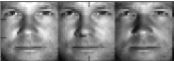
\includegraphics[width=.15\textwidth]{figChap6/Yale_snap.JPG}};
    
\node (in1) [io, below of=start,node distance=1.6cm] {\textbf{Initialize}: $r=0$, Projection matrix $\bm{Q}_{0}$ using PCA, $\bm{U}_{0}=\bm{Y}$, $\bm{T}_{0}=\bm{Y}$, $\bm{V}_{0}=0$};

\node (pro1) [process, below of=in1,node distance=1.6cm] {\begin{tabular}{l} Update Projection matrix $\bm{Q}$ \\ Update twin matrix $\bm{U}$ \\ 
Update mapping matrix $\bm{V}$\end{tabular}};

\node (pro2b) [process, below of=pro1, node distance=1.45cm] { % xshift=2.5cm
\begin{tabular}{l} Update the classwise mean matrix $\overline{\bm{M}}$ \\
Update the columns of matrix $\bm{T}$\end{tabular}};

\node (dec1) [decision, below of=pro2b, node distance=2.0cm] {$r\geq N_{max}$};

\node (out1) [io, below of=dec1,node distance=2.0cm] { \textbf{Output}: \begin{tabular}{l}  Projection matrix $\bm{Q}=\bm{Q}_{r}$ \\ Twin matrix $\bm{U}=\bm{U}_{r}$ \end{tabular}};

\draw [arrow] (start) -- (in1);
\draw [arrow] (in1) -- (pro1);
\draw [arrow] (pro1)  --  (pro2b);
%\draw [arrow] (pro2b)  --  (pro1);
\draw [arrow] (pro2b) --  (dec1);

\draw [arrow] (dec1) --  (out1);

\node (v1) at (0.88,-6.65) {};
\node (v2) at (3.48,-6.65) {};
\draw  [thick] (v1) edge (v2);
\node (v3) at (3.34, -6.80){};
\node (v4) at (1.815, -3.12){};
\draw [arrow] (v3) |- (v4);
%\node (v2) at (-2.4,-3.61) {};
%\node (v1) at (-2.4,-2.86) {};
%\draw  [arrow] (v1) -- (v2);
%\node (v3) at (-3.38,-6.99) {};
%\node (v4) at (-3.38,-3.4) {};
%\draw  [arrow] (v3) -- (v4);
%\node (v6) at (-3.52,-4.1) {};
%\node (v5) at (-2.88,-4.1) {};
%\draw  [thick] (v5) edge (v6);
%\draw  [arrow] (-2.4,-4.7) -- (-2.4,-5.1) -- (1.13,-5.1) -- (1.13,-4.78);
%\node at (-2.7,-2.39){\em Iterative optimization}
\node at (-3.4,-0.70) {Example data};
\node at (1.32,-6.35) {False};
\node at (-0.44,-7.85) {True};
\node at (-0.82,-5.55) {$r = r + 1$};
%\node at (-2.13,-3.2) {i=1};
%\node at (-1.6,-3.9) {i=i+1};
\end{tikzpicture}}
\caption{Flowchart of the proposed TRLSR model.}
\label{Fig: TRLSR Flow chart}
\end{figure}
%
\subsection{Optimization}
%
We use an iterative optimization approach to solve~\eqref{eq: TRLSR_Objective_mod} by iteratively updating $\bm{Q}$, $\bm{M}_{k}$, $\bm{U}$, $\bm{V}$, and $\bm{T}$. We can rewrite the objective function in~\eqref{eq: TRLSR Final_Objective} as:
%
\begin{align}
    \label{eq: TRLSR_Simple_formulation}
     \Psi = \|\bm{Q}^{T}\bm{X} - \bm{U} - \overline{\bm{M}} \|_{F}^{2} + \alpha \| \bm{T} - \bm{V} \bm{U}\|_{F}^{2} + \gamma \| \bm{Q}\|_{2,1}   + \tau \| \bm{V} \|_{F}^{2} 
\end{align}
%
where $\overline{\bm{M}} = \left[\bm{M}_{1}, \bm{M}_{2},\dots,\bm{M}_{c}\right]$. Each of the variables are updated alternately while the other variables are kept fixed. The key steps are explained next and the iteration stops when the convergence criteria are met.
 
\noindent\textbf{Update $\bm{Q}$}: By keeping $\bm{U}$, $\bm{V}$ fixed, we can rewrite~\eqref{eq: TRLSR_Simple_formulation} as:
%-----------------------------------%
\begin{equation}
    \label{eq: TRLSR_Update_Q}
    \Psi(\bm{Q})  = \| \bm{Q}^{T}\bm{X} - \bm{U} - \overline{\bm{M}}\|_{F}^{2} + \gamma\|\bm{Q}\|_{2,1}
\end{equation}
%
Setting the partial derivative of~\eqref{eq: TRLSR_Update_Q} with respect to $\bm{Q}$ to zero, we obtain the following closed-form expression for updating $\bm{Q}$:
%
%-------------------------------------%
\begin{equation}
    \label{eq: TRLSR_Define_Q}
    \bm{Q}^{r+1} = \left(\bm{X}\bm{X}^{T} + \gamma \bm{Z}\right)^{-1} \left(\bm{X} \left(\bm{U} + \overline{\bm{M}}\right)^{T} \right)
\end{equation}
%----------------------------------%
%
where $r$ is the current iteration and $\bm{Z}$ is a diagonal matrix with $\bm{Z}_{i,i}=\frac{1}{2\|\bm{q}^{i}\|_{2}}$ for $i= 1,2,\dots,m$. If $\frac{1}{\| \bm{q}^{i}\|_{2}}=0$, then we assume $\bm{Z}_{i,i}=0$.

\noindent\textbf{Update $\bm{U}$}: We update $\bm{U}$ by minimizing the following:
%------------------------------%
\begin{align}
    \label{eq: TRLSR_Update_U}
   \Psi (\bm{U}) =  \| \bm{Q}^{T}\bm{X} - \bm{U} - \overline{\bm{M}} \|_{F}^{2} + \alpha \| \bm{T} - \bm{V} \bm{U} \|_{F}^{2}
\end{align}
%---------------------------------%
which has a closed-form solution given by:
%
\begin{align}
    \label{eq: TRLSR_Define_U}
    \bm{U}^{r+1} = \left(\bm{I}_{c} + \alpha \bm{V}^{T} \bm{V}\right)^{-1} \left( (\bm{Q}^{T} \bm{X} - \overline{\bm{M}} ) +  \alpha \bm{V}^{T} \bm{Y} \right)
\end{align}
%
where $\bm{I}_{c}$ is the identity matrix of dimensions $c\times c$.  

\noindent\textbf{Update $\bm{V}$}: We update $\bm{V}$ by minimizing the following:
%--------------------------%
\begin{equation}
    \label{eq: TRLSR_Update_V}
    \Psi(\bm{V}) = \alpha \| \bm{T} - \bm{V} \bm{U} \|_{F}^{2} + \tau \| \bm{V} \|_{F}^{2}
\end{equation}
%--------------------------%
The closed-form expression for updating $\bm{V}$ is given by:
%--------------------------%
\begin{equation}
    \label{eq: TRLSR_Define_V}
    \bm{V}^{r+1} = \bm{T}\bm{U}^{T}(\bm{U}\bm{U}^{T} + \tau\bm{I}_{c} )
\end{equation}
%
\noindent\textbf{Update $\bm{T}$}: To update $\bm{T}$, we keep $\bm{U}$ and $\bm{V}$ fixed, and minimize:
%
\begin{align}
    \begin{split}
        \label{eq: TRLSR_Define_T}
        \Psi(\bm{T}) = \| \bm{T} - \bm{V} \bm{U} \|_{F}^{2} = \|\bm{T} - \bm{H} \|_{F}^{2}  
    \end{split}
\end{align}
%
where $\bm{H}=\bm{VU} \in \Re^{c \times n}$. This results in $n$ mutually independent constrained sub-problems for each column vector $\bm{t}_{i} \in \Re^{c}$ which can be expressed as:
%
\begin{align}
\begin{split}
    \label{eq: TRLSR_Subproblem_T}
    \min_{\bm{t}_{i}} \, \| \bm{h}_{i} - \bm{t}_{i} \|_{2}^{2} \quad \text{s.t.} \enskip \bm{T}_{l_{i},i} - \max_{j \neq i} \bm{T}_{j,i} \geq 1
    %, \forall i = 1,2,\dots,n 
\end{split}
\end{align}
%
As in~\cite{ReLSR}, we can express $\bm{T}$ as:
%
\begin{equation}
\label{eq: TRLSR_target_def}
   \bm{T}_{j,i} =
   \begin{cases}
H_{j,i} + \Delta_{i} \enskip \qquad \quad \qquad \text{if} \enskip j = l_{i}  \\
H_{j,i} + \min (\Delta_{i} - g_{j}, 0) \enskip \text{if} \enskip j \neq l_{i}
\end{cases}
\end{equation}
%
where $\Delta_{i} = \bm{H}_{l_{i},i} - \bm{T}_{l_{i},i}$ is the step parameter, and $g_{j} = \bm{H}_{j,i} + 1 - \bm{H}_{l_{i}, i}$ is an indicator function, i.e. if $g_{j} \leq 0$, class $j$ and class $l_{i}$  satisfy the margin constraint. Using the notation in~\eqref{eq: TRLSR_target_def}, the minimization problem~\eqref{eq: TRLSR_Subproblem_T} can be rewritten as:
%
\begin{align}
    \label{eq: TRLSR_Gamma_min}
     \min_{\Delta_{i}}\, \Gamma (\Delta_{i}) = \Delta_{i}^{2} + \sum_{j=1,j \neq l_{i}}^{c} \left(\min (\Delta_{i} - g_{j}, 0)\right)^{2} 
\end{align}
%
Taking the derivative of $\Gamma (\Delta_{i})$ with respect to $\Delta_{i}$ we obtain: 
%
\begin{align}
   \label{eq: TRLSRGamma_derivative}
    \Gamma^{\prime} (\Delta_{i}) = 2 \left(\Delta_{i} + \sum_{j=1,j \neq l_{i}}^{c} (\min (\Delta_{i} - g_{j}, 0)) \right)
\end{align}
%
The optimal solution of~\eqref{eq: TRLSR_Gamma_min} is an extreme point that satisfies $\Gamma^{\prime} (\Delta_{i}) = 0$. By setting $\Gamma^{\prime} (\Delta_{i})=0$, the optimal $\Delta_{i}$ is given as~\cite{ReLSR}:
%
\begin{align}
    \label{eq: TRLSR_Optimal_Delta}
    \Delta_{i} = \frac{\sum_{j=1,j \neq l_{i}}^{c} g_{j} \Phi(g_{j})}{1 + \sum_{j=1,j \neq l_{i}}^{c} \Phi(g_{j})}
\end{align}
%
where $\Phi(g_{j}) = 1$ for $\Gamma^{\prime}(\Delta_{i}) > 0$ and is $0$ otherwise. The iterative optimization procedure is summarized in Algorithm \ref{Algo: TRLSR}.
%%====================================================%%
\begin{algorithm}
\SetAlgoLined
\textbf{Input}: Training data matrix $\bm{X}$; label matrix $\bm{Y}$; parameters $\alpha$, $\gamma$, and $\tau$.\\
\textbf{Initialization}: Initialize orthogonal matrix $\bm{Q}$ using PCA, $\bm{U}=\bm{Y}$,$\bm{V}=\bm{0}$, $\bm{T} = \bm{Y}$\\
Set $r = 0$; \\
\While{not converged}{
Update $\bm{Q}$, $\bm{U}$, and $\bm{V}$ using~\eqref{eq: TRLSR_Define_Q},~\eqref{eq: TRLSR_Define_U}, and~\eqref{eq: TRLSR_Define_V}.\\
Update classwise mean matrix $\overline{\bm{M}}$.\\
Update the columns of $\bm{T}$.\\
$r = r + 1$;}
\textbf{Output}: Projection matrix $\bm{Q}$.
\caption{TRLSR framework}
\label{Algo: TRLSR}
\end{algorithm}
%%=======================================================%%

After solving~\eqref{eq: TRLSR_Simple_formulation}, we obtain the projection matrix $\bm{Q}$, which can be used for classification. For instance, if $\bm{x}_{\text{test}}$ is the test sample, then the transformed features are $\bm{Q}^{T}\bm{x}_{\text{test}}$ and we use the $K$-nearest neighbor classifier to classify the sample. 
%
%=============================================================================%
\begin{table}
\caption{Mean classification rate ($\%$) of LR-DRR method for Ex Yale B data set.}
\label{table: LRDRR_Accuracy_Yale_train}
\centering
%\small
\begin{tabular}{|c|cccc|}
\hline
\multirow{2}{*}{Alg.} & \multicolumn{4}{c|}{Training number ($t_r$)}                                                                                 \\ \cline{2-5} 
                      & \multicolumn{1}{c|}{10}            & \multicolumn{1}{c|}{15}            & \multicolumn{1}{c|}{20}            & 25            \\ \hline
SRC~\cite{SRC}                   & \multicolumn{1}{c|}{85.4}          & \multicolumn{1}{c|}{92.6}          & \multicolumn{1}{c|}{94.4}          & 96.7          \\ \hline
CRC~\cite{CRC}                   & \multicolumn{1}{c|}{86.1}          & \multicolumn{1}{c|}{90.7}          & \multicolumn{1}{c|}{93.0}          & 94.1          \\ \hline
LLC~\cite{LLC}                   & \multicolumn{1}{c|}{79.8}          & \multicolumn{1}{c|}{88.6}          & \multicolumn{1}{c|}{91.5}          & 94.3          \\ \hline
LRC~\cite{LRC}                   & \multicolumn{1}{c|}{81.6}          & \multicolumn{1}{c|}{89.4}          & \multicolumn{1}{c|}{92.4}          & 93.6          \\ \hline
LRLR~\cite{LRLR_SLRR}                  & \multicolumn{1}{c|}{84.6}          & \multicolumn{1}{c|}{82.0}          & \multicolumn{1}{c|}{83.8}          & 85.0          \\ \hline
SLRR~\cite{LRLR_SLRR}                  & \multicolumn{1}{c|}{87.9}          & \multicolumn{1}{c|}{82.3}          & \multicolumn{1}{c|}{84.2}          & 85.1          \\ \hline
DLSR~\cite{DLSR}                  & \multicolumn{1}{c|}{86.2}          & \multicolumn{1}{c|}{92.3}          & \multicolumn{1}{c|}{94.7}          & 95.8          \\ \hline
ReLSR~\cite{ReLSR}                 & \multicolumn{1}{c|}{87.5}          & \multicolumn{1}{c|}{92.9}          & \multicolumn{1}{c|}{95.3}          & 96.2          \\ \hline
LRRR~\cite{LRLR_SLRR}                  & \multicolumn{1}{c|}{78.6}          & \multicolumn{1}{c|}{82.3}          & \multicolumn{1}{c|}{83.6}          & 85.4          \\ \hline
SLRR~\cite{LRLR_SLRR}                  & \multicolumn{1}{c|}{78.0}          & \multicolumn{1}{c|}{82.3}          & \multicolumn{1}{c|}{84.2}          & 85.1          \\ \hline
LRSI~\cite{LRSI}                 & \multicolumn{1}{c|}{87.1}          & \multicolumn{1}{c|}{92.7}          & \multicolumn{1}{c|}{94.2}          & 96.1          \\ \hline
SALPL~\cite{SALPL}                 & \multicolumn{1}{c|}{88.3}          & \multicolumn{1}{c|}{93.3}          & \multicolumn{1}{c|}{95.8}          & 97.1          \\ \hline
CBDS~\cite{CBDS}                  & \multicolumn{1}{c|}{85.8}          & \multicolumn{1}{c|}{93.1}          & \multicolumn{1}{c|}{95.8}          & 96.3          \\ \hline
LR-DRR                & \multicolumn{1}{c|}{\textbf{91.7}} & \multicolumn{1}{c|}{\textbf{95.8}} & \multicolumn{1}{c|}{\textbf{97.4}} & \textbf{97.9} \\ \hline
\end{tabular}
\end{table}
%%================================================================================%%
%%=======================================================%%
\section{Experimental Results of LR-DRR}
\label{sec: Chap6_LRDRR_result}
%
To evaluate the performance of the proposed LR-DRR framework, we conduct experiments for face recognition, object classification, and scene recognition applications. We compare the performance of LR-DRR with state-of-the-art approaches on: (i) two face recognition data sets: Extended Yale B~\cite{Yale_B} and AR~\cite{Data_AR}, (ii) two object recognition data sets: COIL-20~\cite{Data_COIL} and Caltech-101~\cite{Caltech101}, and (iii) $15$-Scene data set~\cite{15scene_1} for scene classification. As discussed in Section~\ref{sec: Chap2_Literature_datasets}, we use the spatial pyramid features for the 15-Scene data set provided in~\cite{LCKSVD, 15scene_3}. 
%-----------------------------------------------------------------------------%
We compare the proposed LR-DRR technique with the following state-of-the-art methods: (i) regression-based methods: SRC~\cite{SRC}, LLC~\cite{LLC}, LRC~\cite{LRC}, CRC~\cite{CRC}, DLSR~\cite{DLSR}, ReLSR~\cite{ReLSR}, (ii) low-rank based methods: CBDS~\cite{CBDS}, LRLR~\cite{LRLR_SLRR}, LRRR~\cite{LRLR_SLRR}, LatLRR~\cite{LatLRR}, SALPL~\cite{SALPL}, and (iii) dictionary-based methods: KSVD~\cite{KSVD} and D-KSVD~\cite{DKSVD}. We use the author-provided source codes for SALPL, DLSR, ReLSR, LatLRR, K-SVD, LC-KSVD, D-KSVD, and GReLSR, whereas we implemented SVM. For a fair comparison, results of SRC, CRC, LLC, LRLR, and LRRR, are taken from their source publications under similar experimental settings. For all the data sets, we set $\mu = 1\mathrm{e}{-2}$, $\rho = 1.03$, and $\mu_{\text{max}} = 1\mathrm{e}{5}$. We repeat each set of experiments $10$ times with random selection of the training and test data samples, and report the mean classification rates. For Extended Yale B and COIL-20 data sets, we randomly select $10$ and $15$ samples from each class for training and the rest are used for testing. For each training number, the mean classification rate is shown in Table~\ref{table: LRDRR_Accuracy_Yale_train}.  
\begin{table}
\small
\caption{Mean classification rate ($\%$) of LR-DRR method for Caltech-101 data set}
\label{table: LRDRR_Accuracy_Caltech}
\centering
\begin{tabular}{|c|c|c|c|c|}
\hline
\multirow{2}{*}{Algorithm} & \multicolumn{4}{c|}{Training number ($t_r$)}\\
\cline{2-5}
 & 5              & 10             & 15             & 20\\
\hline            
LLC \cite{LLC} & 51.5           & 59.8          & 65.4          & 67.7\\
\hline
SRC \cite{SRC} & 48.8           & 60.1           & 64.9           & 67.7\\
\hline
K-SVD \cite{KSVD} & 49.8           & 59.8           & 65.2           & 68.7\\
\hline
D-KSVD \cite{DKSVD} & 49.6           & 59.5           & 65.1           & 68.6\\
\hline
LC-KSVD1 \cite{LCKSVD} & 53.5      & 61.9           & 66.8           & 70.3\\
\hline
LC-KSVD2 \cite{LCKSVD} & 54.0           & 63.1           & 67.7           & 70.5\\
\hline
SALPL \cite{SALPL} & 56.3           & 64.4           & 68.3           & \textbf{72.0}\\
\hline
LR-DRR & \textbf{59.7} & \textbf{66.3} & \textbf{70.4} & 71.6\\ 
\hline
\end{tabular}
\end{table}
%============================================================================%%
%
\begin{table}
\caption{Comparison of mean classification rates (in $\%$) of LR-DRR method.}
\label{table: LRDRR_Accuracy_15_AR}
\centering
\begin{tabular}{|c|c|l|c|c|c|c|}
\hline
Algorithm & \multicolumn{2}{c|}{AR} & 15-Scene & Algorithm & AR & 15-Scene\\ 
\hline 
LRC \cite{LRC} & \multicolumn{2}{c|}{94.5}           & 91.9           & LRLR \cite{LRLR_SLRR}  & -    & 94.5\\ 
\hline
CRC \cite{CRC}      & \multicolumn{2}{c|}{97.3}           & 92.3    & LatLRR \cite{LatLRR} & 97.6 & 91.5\\ 
\hline
LC-KSVD1 \cite{LCKSVD} & \multicolumn{2}{c|}{92.5}           & 93.7  & CBDS \cite{CBDS}  & -    & 95.7\\ 
\hline
LC-KSVD2 \cite{LCKSVD} & \multicolumn{2}{c|}{93.7}           & 92.9  & SVM \cite{SVM}   & 96.7 & 93.6     \\ 
\hline
ReLSR\cite{ReLSR}    & \multicolumn{2}{c|}{94.5}          & 95.4  & LLC \cite{LLC}    & 88.7 & 89.2     \\ 
\hline
DLSR \cite{DLSR}     & \multicolumn{2}{c|}{97.6}           & 95.9  & SRC \cite{SRC}   & 97.5 & 91.8     \\ 
\hline
LRSI \cite{LRSI}     & \multicolumn{2}{c|}{-}              & 92.4  & SLRR \cite{LRLR_SLRR}  & -    & 89.6     \\ 
\hline
LR-DRR & \multicolumn{2}{c|}{\textbf{98.7}} & \textbf{98.6} &     &      & \\ 
\hline
\end{tabular}
\end{table}
%
%
For Caltech-101, the training number is varied from $5$ to $20$ with the remaining samples constituting the test set. The mean classification rate is shown in Table~\ref{table: LRDRR_Accuracy_Caltech}. Unlike the low-rank and sparse representation based methods whose primary aim is to improve the data representation, the proposed LR-DRR technique encourages the extraction of discriminative features while also addressing the problem of overfitting resulting in superior classification performance. Following the common experimental
settings used in ~\cite{LCKSVD, RLSL}, we randomly select $20$ and $100$ images from each class for training and the rest are used for testing on the AR and 15-scene data sets, respectively. For comparison, SRC, CRC, LRC methods are used with a dictionary size of $450$ i.e., $30$ items for each class. These methods represent input test samples as a linear combination of the learned dictionary items, and then use the representation coefficients for classification. Table~\ref{table: LRDRR_Accuracy_15_AR} shows the mean classification rates for face recognition and scene classification tasks.

From these results, superiority of the proposed LR-DRR technique is evident compared with the state-of-the-art methods. LR-DRR uses the double relaxed regression for the target matrix and a low-rank error term, thereby offering additional degrees of freedom in optimizing the projection matrix with better class margins, resulting in improved performance. To study the effect of double relaxation, we conduct an experiment without the matrix $\mathbf{E}$ by solving:
%
\begin{align}
   \label{eq: LRDRR_Without_E}
   \min_{\mathbf{Q}, \mathbf{U}, \mathbf{V}} \, \frac{1}{2} \| \mathbf{Y} - \mathbf{V} \mathbf{U} \|_{F}^{2} + \alpha \| \mathbf{Q}^{T} \mathbf{X} - \mathbf{U} \|_{F}^{2} + \gamma \| \mathbf{Q} \|_{2,1} + \tau \| \mathbf{V} \|_{F}^{2}
\end{align}
%--------------------------------------------------%
For the Caltech-101 data set with training number $5$, solving~\eqref{eq: LRDRR_Without_E} results in a mean classification of $57\%$ which is significantly lower than $59.7\%$ (refer Table~\ref{table: LRDRR_Accuracy_Caltech}) achieved using the double relaxation. Similarly, for the Extended Yale B data set, classification rates for training number $10$ without and with $\mathbf{E}$ are $90\%$ and $91.7\%$ (refer Table~\ref{table: LRDRR_Accuracy_Yale_train}), respectively.

Next, we visualize distribution of the transformed features using the t-SNE algorithm~\cite{TSNE}. Fig.~\ref{fig: LRDRR_TSNE} shows the features extracted by LR-DRR for a few data samples from the Extended Yale B data set. It is clear that LR-DRR efficiently classifies all the data samples into their respective subspaces. This validates our claim of the proposed LR-DRR technique being able to capture discriminative and compact features from the original data samples.
%
\begin{table}
\caption{Mean classification rate ($\%$) of LR-DRR method for COIL-20 dataset}
\label{table: LRDRR_Accuracy_Coil_dataset}
\centering
\begin{tabular}{|c|cccc|}
\hline
\multirow{2}{*}{Alg.} & \multicolumn{4}{c|}{Training number ($t_r$)}                                                                                  \\ \cline{2-5} 
                      & \multicolumn{1}{c|}{10}            & \multicolumn{1}{c|}{15}             & \multicolumn{1}{c|}{20}            & 25            \\ \hline
SRC                   & \multicolumn{1}{c|}{91.2}          & \multicolumn{1}{c|}{94.5}           & \multicolumn{1}{c|}{96.2}          & 97.2          \\ \hline
CRC                   & \multicolumn{1}{c|}{87.7}          & \multicolumn{1}{c|}{91.3}           & \multicolumn{1}{c|}{92.2}          & 94.2          \\ \hline
LRC                   & \multicolumn{1}{c|}{92.0}          & \multicolumn{1}{c|}{95.6}           & \multicolumn{1}{c|}{97.2}          & 98.2          \\ \hline
LRLR                  & \multicolumn{1}{c|}{83.0}          & \multicolumn{1}{c|}{86.9}           & \multicolumn{1}{c|}{85.7}          & 89.2          \\ \hline
SLRR                  & \multicolumn{1}{c|}{83.9}          & \multicolumn{1}{c|}{90.2}           & \multicolumn{1}{c|}{90.8}          & 93.8          \\ \hline
DLSR                  & \multicolumn{1}{c|}{92.8}          & \multicolumn{1}{c|}{\textbf{96.22}} & \multicolumn{1}{c|}{97.3}          & 97.8          \\ \hline
ReLSR                 & \multicolumn{1}{c|}{91.9}          & \multicolumn{1}{c|}{95.4}           & \multicolumn{1}{c|}{96.6}          & 97.0          \\ \hline
LR-DRR                & \multicolumn{1}{c|}{\textbf{94.4}} & \multicolumn{1}{c|}{95.9}           & \multicolumn{1}{c|}{\textbf{97.7}} & \textbf{98.3} \\ \hline
\end{tabular}
\end{table}
%
%----- Tsne Visualization ---------%
\begin{figure}
\centering
\subfigure[Original samples]{\label{fig:Orig_tsne}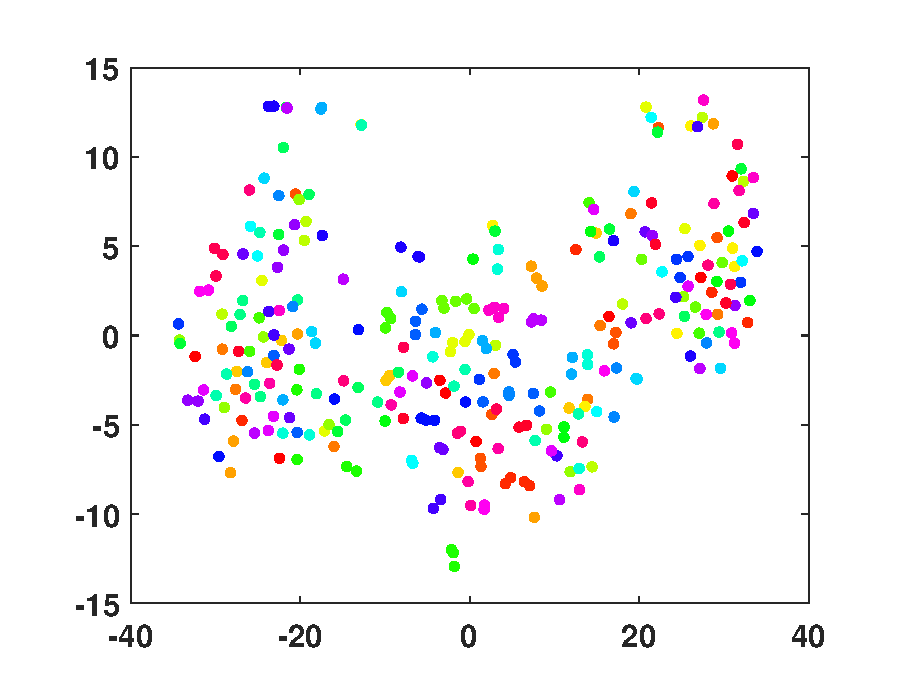
\includegraphics[keepaspectratio,width=0.49\textwidth,trim=0 0 0 0,clip]{figChap6/Orig_tsne_8.eps}}
\subfigure[LR-DRR algorithm]{\label{fig:LSR_tsne}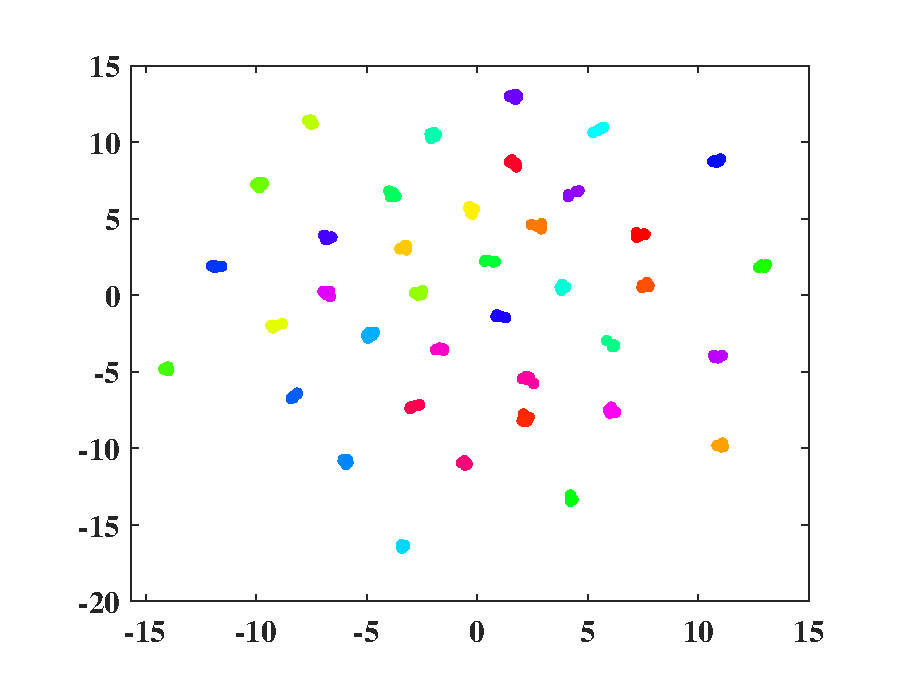
\includegraphics[keepaspectratio,width=0.49\textwidth,trim=0 0 0 0,clip]{figChap6/LSR_tsne.eps}}
\caption{t-SNE visualization of the features extracted on the Extended Yale B data set, where $8$ random samples from each subject are used for validation.}
\label{fig: LRDRR_TSNE}
\end{figure}
%---------------------------------%
%---------------------------------%
\begin{figure}
\centering
    \subfigure[15-Scene data set ($t_r=100$)]{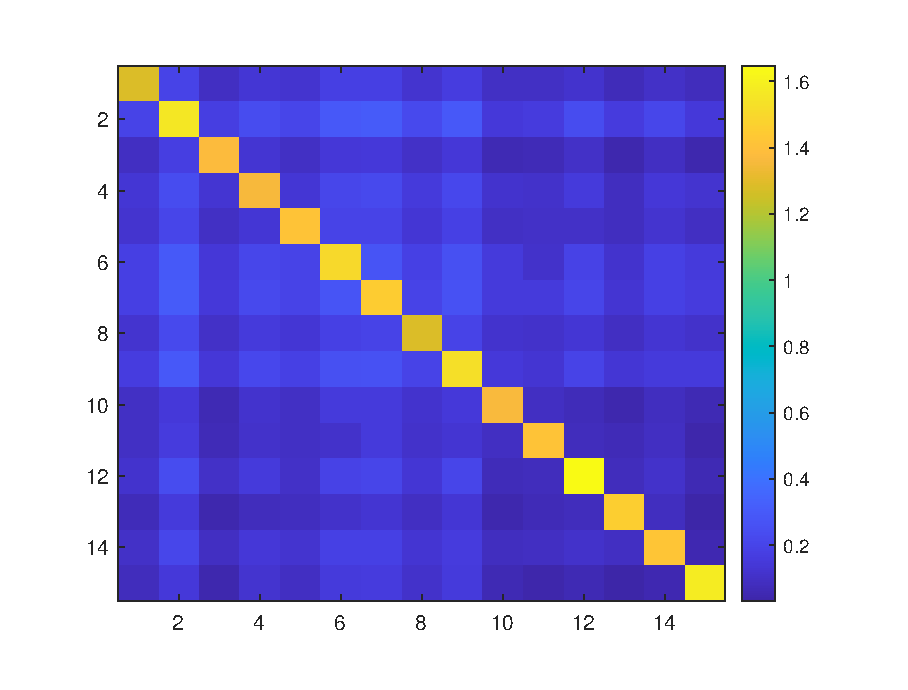
\includegraphics[width=0.48\textwidth]{figChap6/Fig_scene_Vmatrix.eps}} 
    \subfigure[COIL-20 data set ($t_r =10$)]{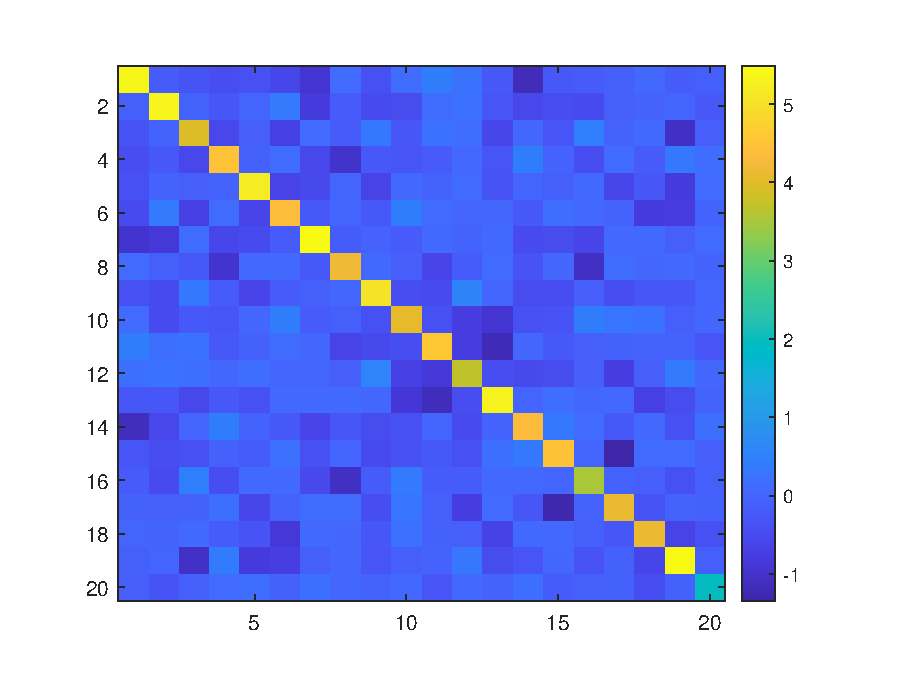
\includegraphics[width=0.48\textwidth]{figChap6/Fig_Coil_Vmatrix.eps}} 
\caption{Visualization of the matrix $\mathbf{V}$ in the LR-DRR problem formulation.}
\label{Fig: LRDRR_Vmatrix_visulization}
%\vspace{-0.2cm}
\end{figure}
%----------------------------------%
\begin{figure}
\centering
    \subfigure[$\alpha$ and $\tau$]{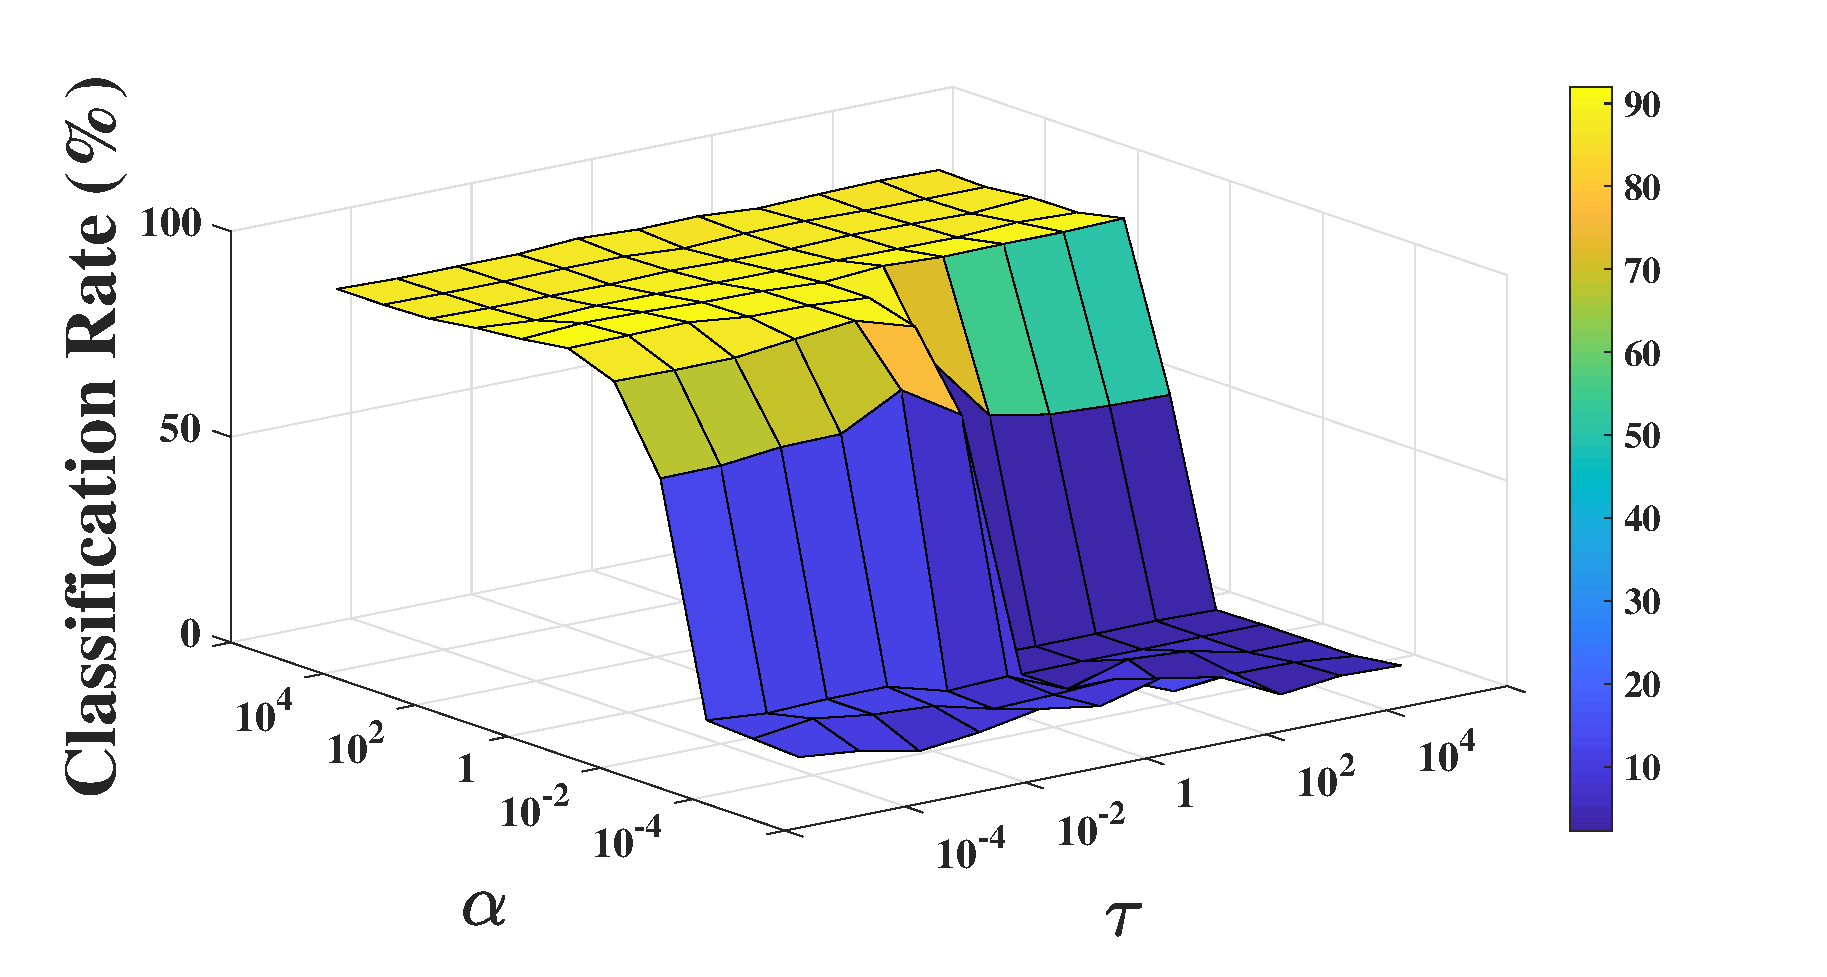
\includegraphics[width=.32\textwidth]{figChap6/Fig_Yale_rate_alpha_tau.eps}} 
   \subfigure[$\beta$ and $\tau$]{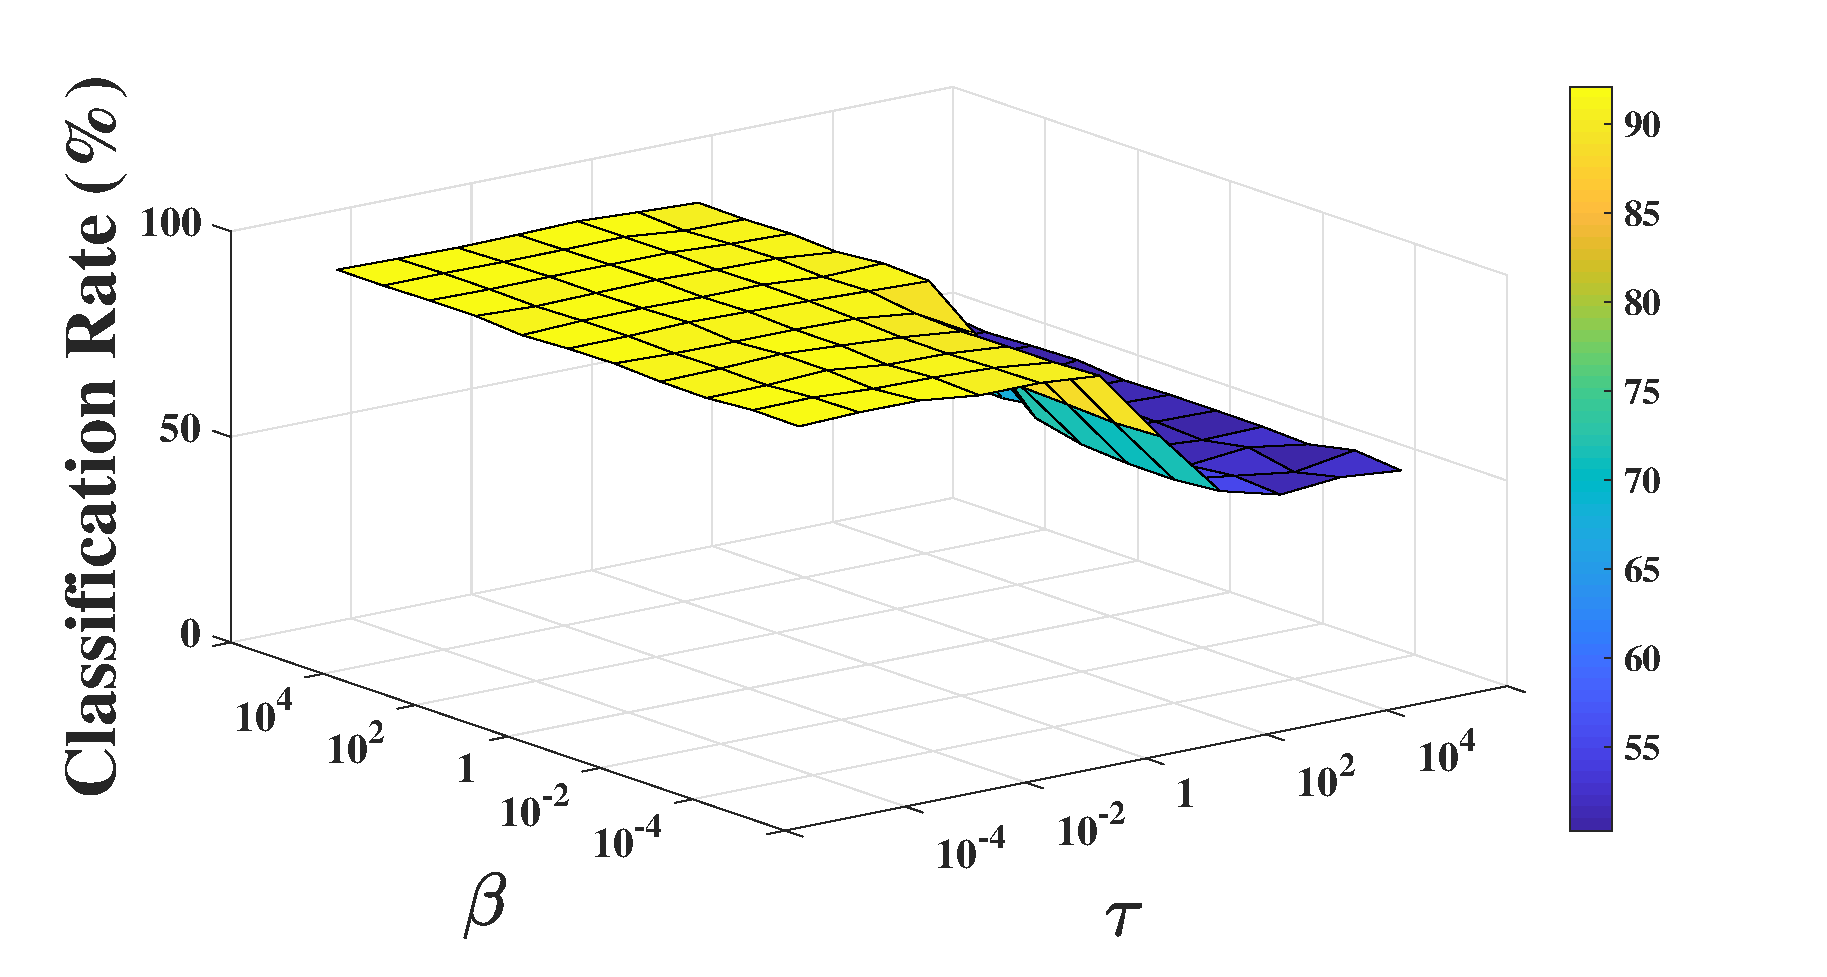
\includegraphics[width=.32\textwidth]{figChap6/Fig_yale_rate_beta_tau.eps}}
\subfigure[$\alpha$ and $\beta$]{\label{fig: Yale_alpha_beta}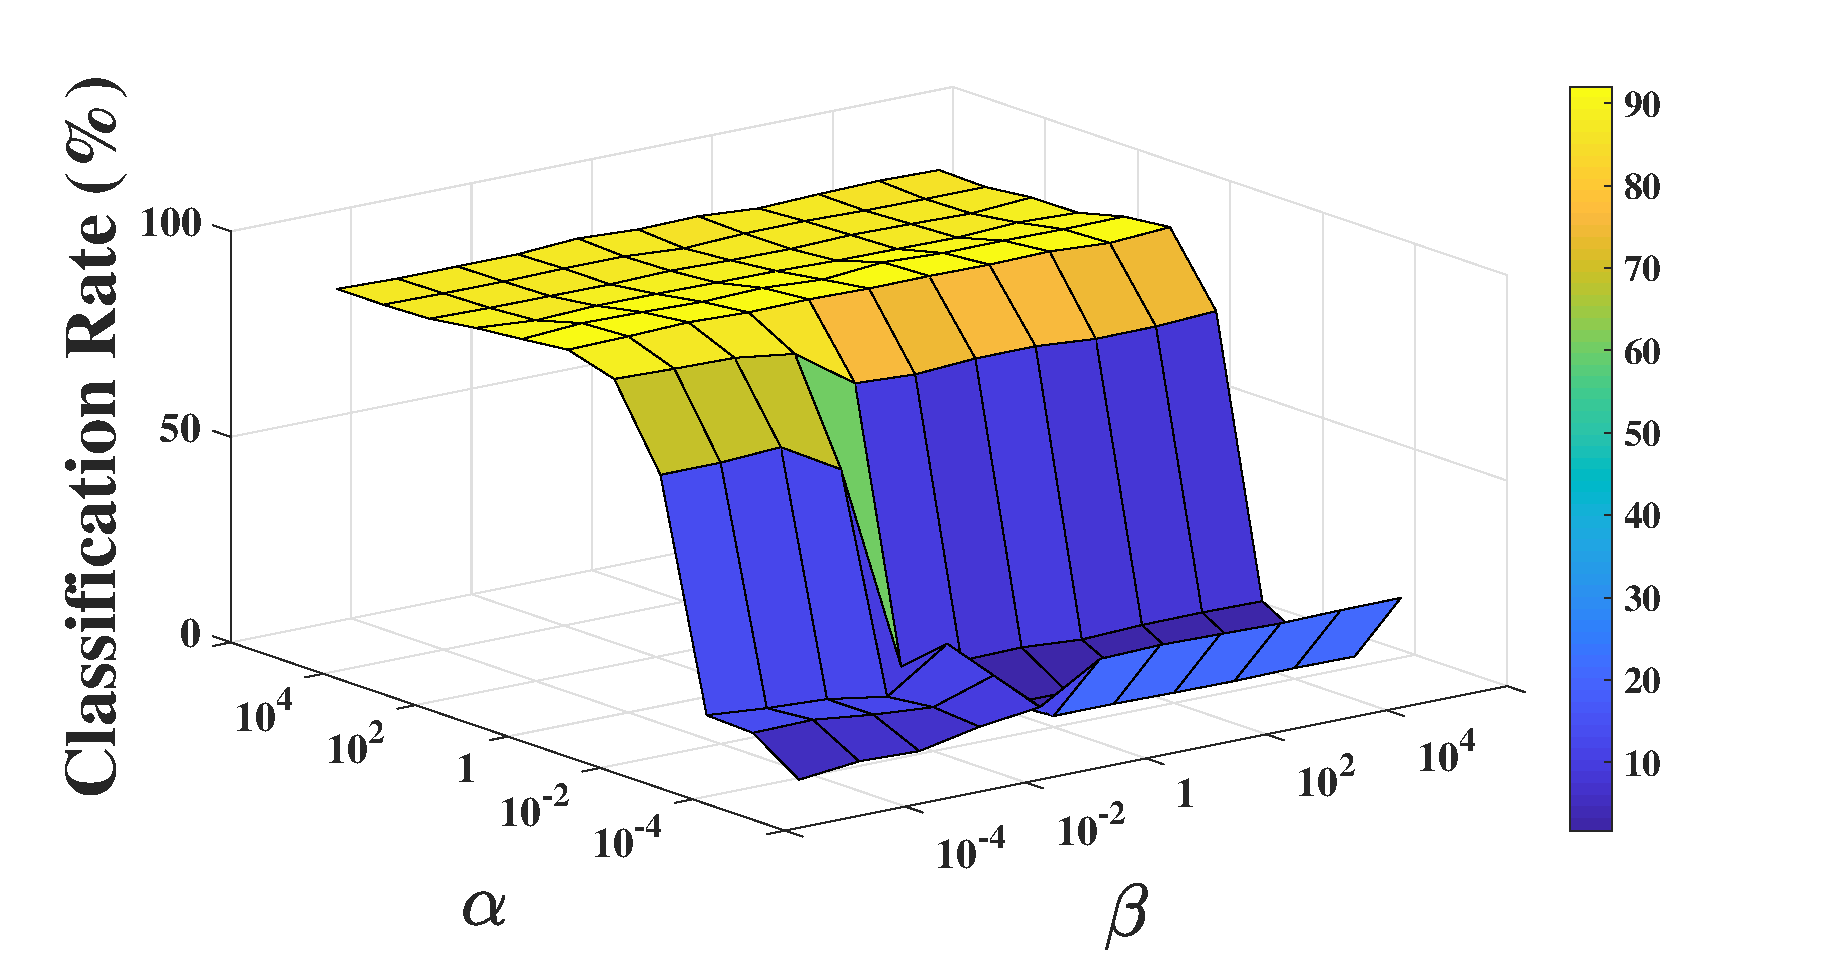
\includegraphics[keepaspectratio,width=0.32\textwidth,trim=0 0 0 0,clip]{figChap6/Fig_Yale_rate_alpha_beta.eps}}
\caption{Classification rate of the LR-DRR method as a function of the parameters $\alpha$, $\beta$ and $\tau$ on the Extended Yale B data set ($t_r=10$).}
\label{Fig: LRDRR_Yale_para}
\end{figure}
%---------------------------------------%
\begin{figure}
\centering
  \begin{tabular}{@{}cc@{}}
    \subfigure[AR data set ($t_r=10$)]{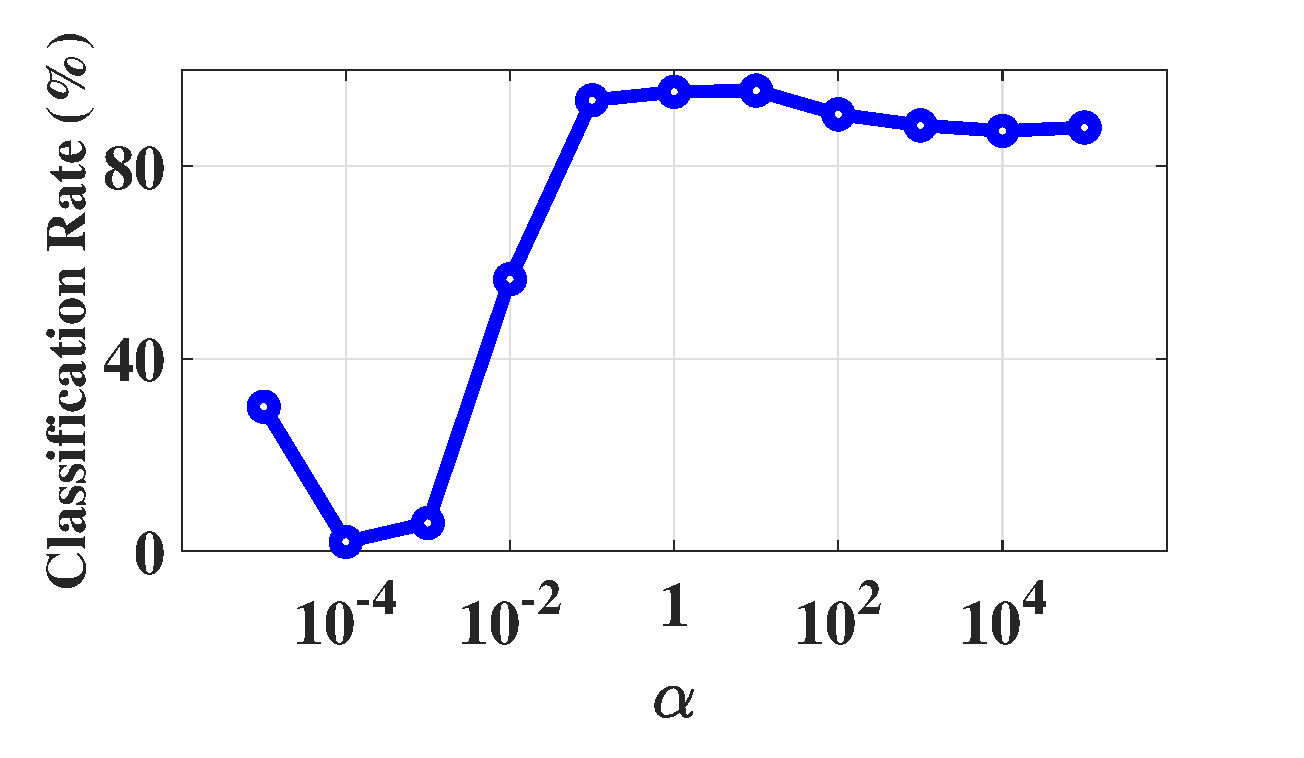
\includegraphics[width=0.48\textwidth]{figChap6/Fig_AR_rate_alpha.eps}} &
    \subfigure[Ex Yale B data set ($t_r=10$)]{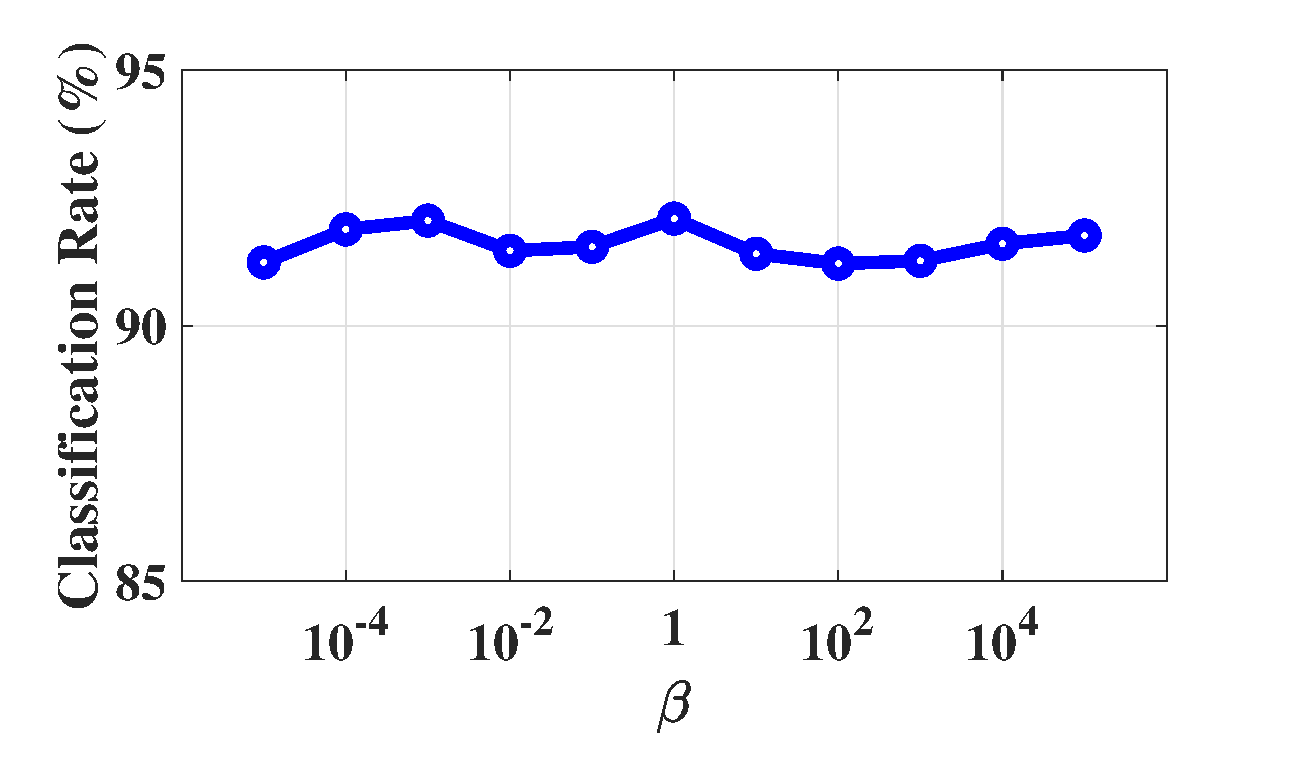
\includegraphics[width=0.48\textwidth]{figChap6/Fig_yale_beta.eps}}\\
    \subfigure[COIL-20 data set ($t_r=10$)]{\label{fig: Coil 20_tau}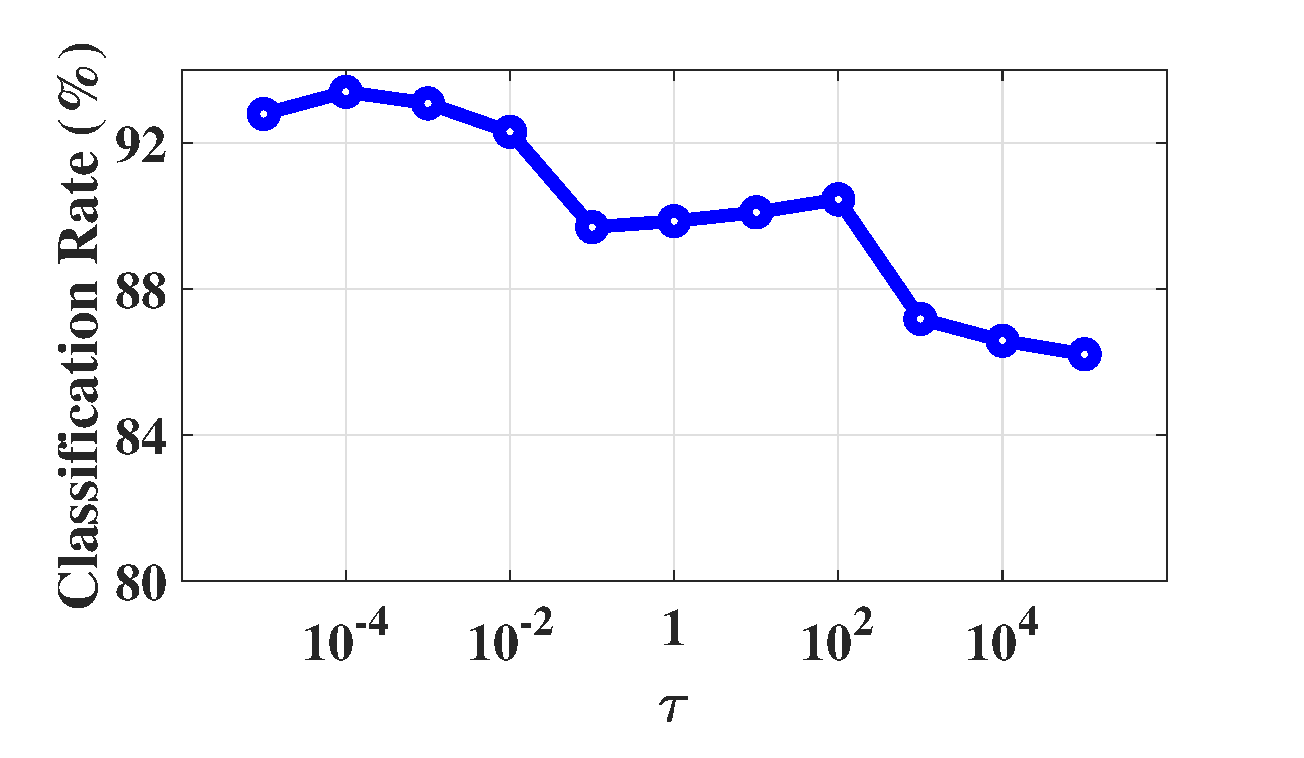
\includegraphics[keepaspectratio,width=0.48\textwidth,trim=0 0 0 0,clip]{figChap6/Fig_Coil_rate_tau.eps}} &
    \subfigure[15-Scene data set ($t_r=100$)]{\label{fig: scene_rate_gamma}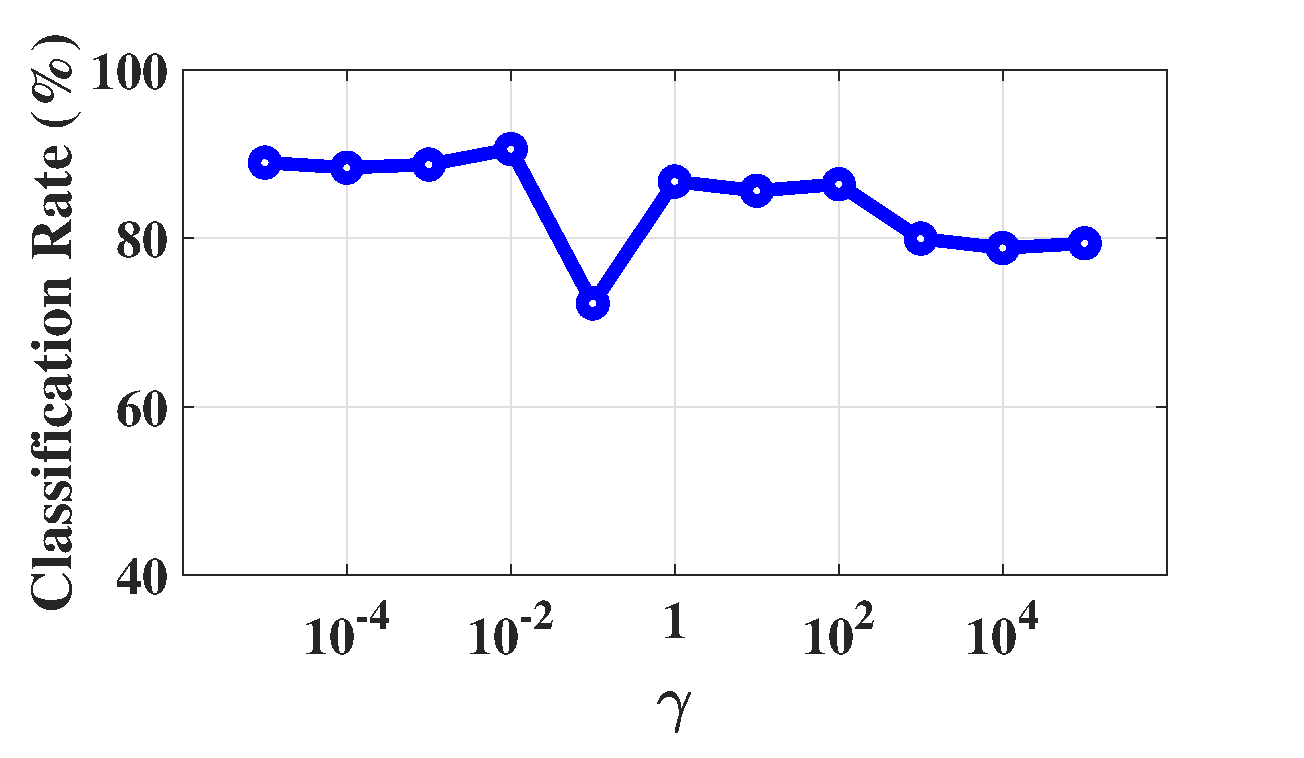
\includegraphics[keepaspectratio,width=0.48\textwidth,trim=0 0 0 0,clip]{figChap6/Fig_scene_rate_gamma.eps}}
  \end{tabular}
\caption{Classification rate of the proposed LR-DRR method as a function of the parameters $\alpha$, $\beta$, $\gamma$, and $\tau$ on different data sets.}
\label{Fig: LRDRR_data_alpha_beta_tau_gamma}
\end{figure}
%------------------------------------------------%

\noindent\textbf{Analysis of the Matrix $\mathbf{V}$}: We next analyze the significance of the matrix $\mathbf{V}$ which provides structural correspondence between $\mathbf{Y}$ and $\mathbf{U}$. It is to be noted that~\eqref{eq: LR-DRR} does not prevent $\mathbf{V}$ from being an identity matrix. However in practical applications, overfitting is a serious problem and $\mathbf{V}$ will turn out to be large and not an identity matrix, which has been observed in our experiments as well. In Fig.~\ref{Fig: LRDRR_Vmatrix_visulization}, we present visualization of the matrix $\mathbf{V}$ for the 15-Scene and COIL-20 data sets. It is seen that the matrix $\mathbf{V}$ has block diagonal structure which indicates that the samples belonging to the same class in $\mathbf{Y}$ and $\mathbf{U}$ will have a correspondence. This ensures structural similarity between $\mathbf{Y}$ and $\mathbf{U}$ as a result of which $\mathbf{U}$ can share the responsibility of the label matrix $\mathbf{Y}$ for better margins. From the results shown in this section, we note that $\mathbf{V}$ allows the model to account for greater variability in the data sets such as when the data is collected in uncontrolled environments. The proposed LR-DRR method outperforms the state-of-the-art techniques by a larger margin on the Caltech-101 data set with images captured in uncontrolled environments than the COIL-20 data set for object recognition applications.

\noindent\textbf{Parameter Sensitivity}: The LR-DRR problem formulation~\eqref{eq: LR-DRR} includes four weight parameters, namely, $\alpha$, $\beta$, $\gamma$, and $\tau$, which need to be tuned appropriately. We conduct experiments on various data sets and the results are depicted in Fig.~\ref{Fig: LRDRR_Yale_para} and Fig.~\ref{Fig: LRDRR_data_alpha_beta_tau_gamma}. We vary the parameter values over the range $\left[ 1\mathrm{e}{-5},1\mathrm{e}{5} \right]$. Fig.~\ref{Fig: LRDRR_data_alpha_beta_tau_gamma} shows the classification rate of the proposed method on different data sets and demonstrates robustness of the proposed method to the individual parameter variations.

%------------------------------------------------------%
\begin{figure}
\centering
 \begin{tabular}{@{}cc@{}}
\subfigure[Extended Yale B data set]{\label{fig: Yale_rate_conv}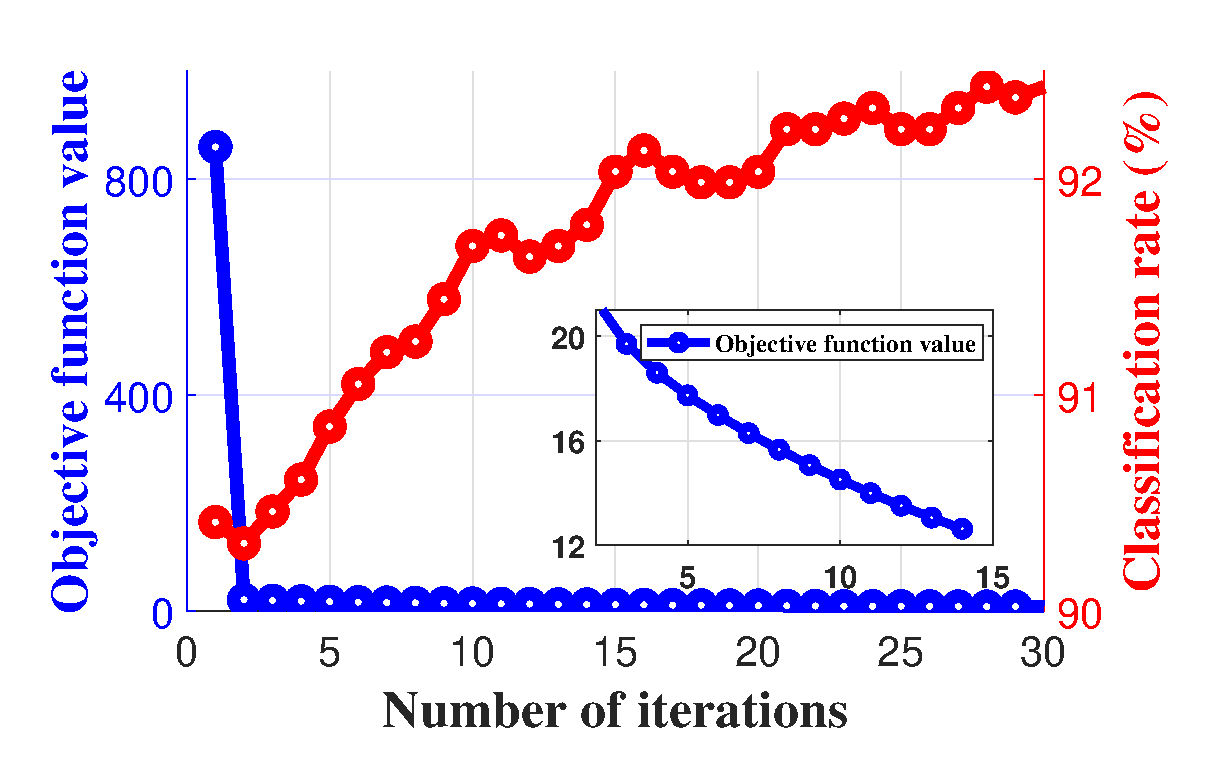
\includegraphics[keepaspectratio,width=0.45\textwidth,trim=0 0 0 0,clip]{figChap6/Fig_Yale_conv.eps}} &
\subfigure[15-Scene data set]{\label{fig: Scene_rate_conv}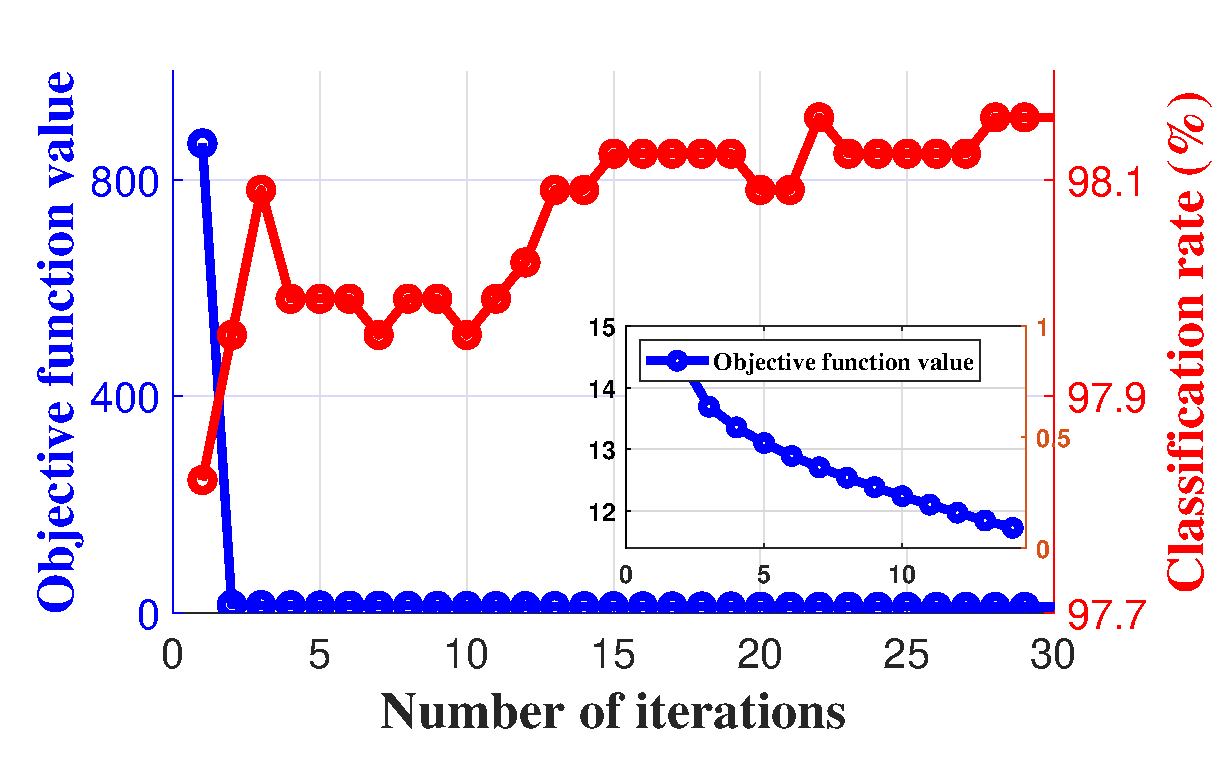
\includegraphics[keepaspectratio,width=0.45\textwidth,trim=0 0 0 0,clip]{figChap6/Fig_scene_conv.eps}} \\
\subfigure[Caltech 101 data set]{\label{fig: Cal_rate_conv}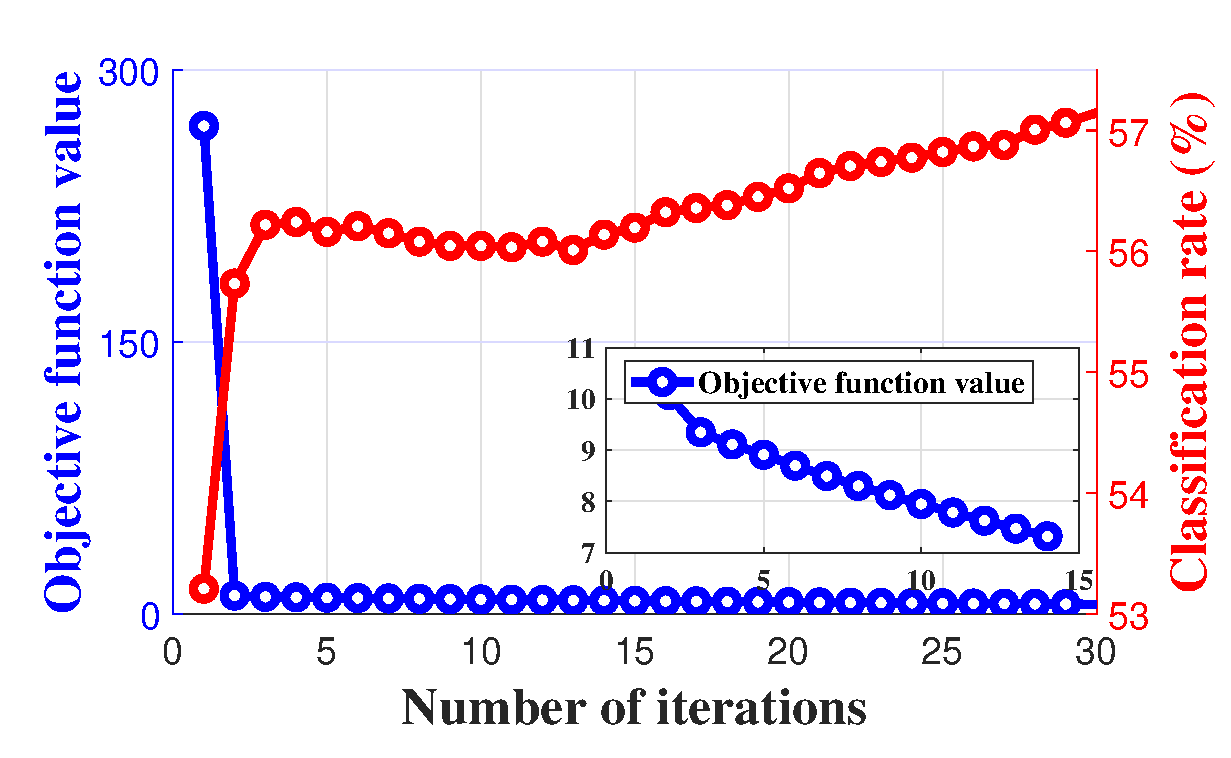
\includegraphics[keepaspectratio,width=0.45\textwidth,trim=0 0 0 0,clip]{figChap6/Fig_Caltech_conv.eps}} &
\subfigure[AR data set]{\label{fig: scene_rate_conv}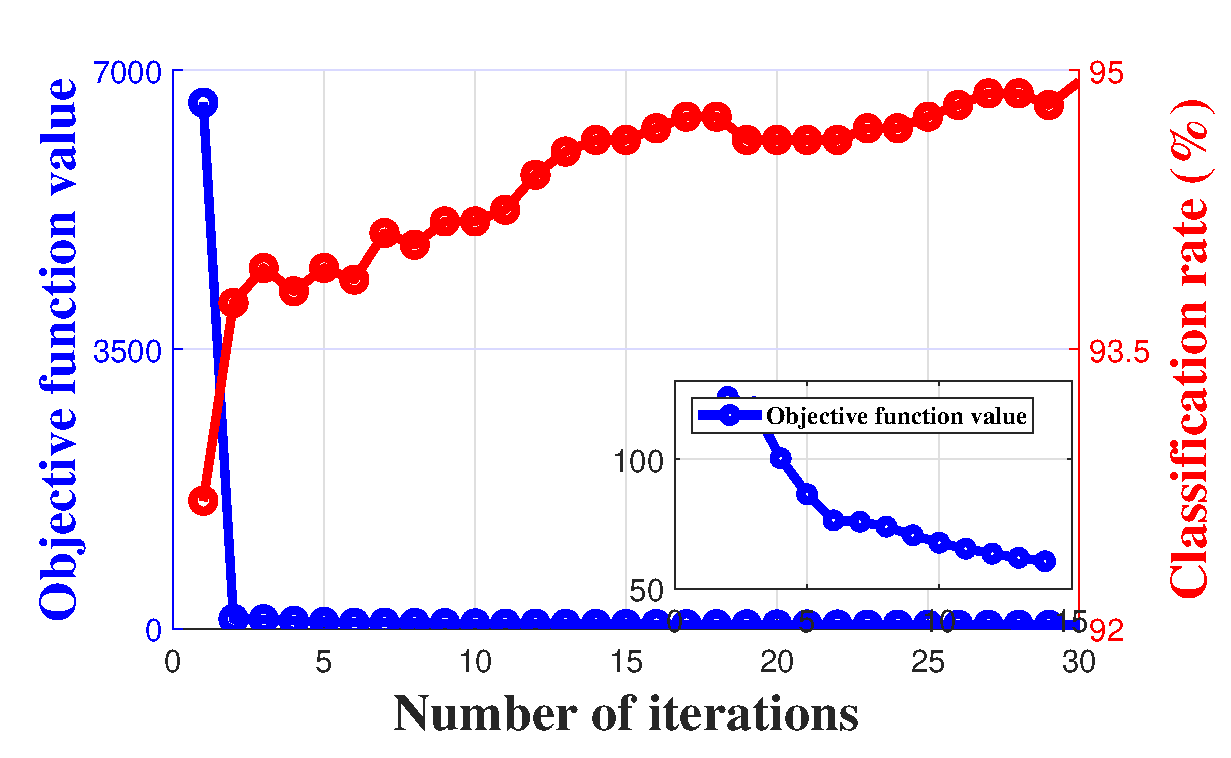
\includegraphics[keepaspectratio,width=0.45\textwidth,trim=0 0 0 0,clip]{ figChap6/Fig_AR_conv.eps}}
  \end{tabular}
\caption{Evolution of objective function value and classification rate with number of iterations for the LR-DRR method.}
\label{fig: LRDRR_Conv_dataset}
\end{figure}
%
Further, Fig.~\ref{Fig: LRDRR_Yale_para} shows the classification rate as a function of the different weight parameters on the Extended Yale B data set. We observe that LR-DRR consistently achieves the best classification performance over the entire range of the parameter $\beta$, and for $\alpha$ in the range $\left[ 1\mathrm{e}{-2}, 1\mathrm{e}{5} \right]$. This indicates that the discriminative power of the regression model significantly affects the performance, and hence, $\alpha$ should be tuned carefully for each data set. Similarly, when the parameter $\tau$ is less than $1\mathrm{e}{-1}$, the classification rate is close to the best achievable performance. This study of parameter variation and classification rate indicates that the proposed LR-DRR model is not very sensitive to the parameter values and gives good performance over a significantly wide range of parameter values. Hence, the proposed model is robust to the parameter variations.\\
%
\textbf{Convergence Study}: We run experiments to study the overall convergence of the proposed method. Fig.~\ref{fig: LRDRR_Conv_dataset} shows the evolution of the objective function value and classification rate with the number of iterations for two data sets. We see that the classification rate increases and the objective function value decreases with the number of iterations. It is also seen that the classification accuracy eventually plateaus after reaching a peak value showing the convergence property of the proposed method.
%
%==========================================================%%
\begin{table}
\caption{Mean classification rate ($\%$) of TRLSR method for Ex Yale B data set}
\label{table: TRLSR_Accuracy_Yale_train}
\centering
\small
\begin{tabular}{|c|cccc|}
\hline
\multirow{2}{*}{Alg.} & \multicolumn{4}{c|}{Training number ($t_r$)}                                                                                      \\ \cline{2-5} 
                      & \multicolumn{1}{c|}{10}             & \multicolumn{1}{c|}{15}             & \multicolumn{1}{c|}{20}             & 25             \\ \hline
SRC~\cite{SRC}                   & \multicolumn{1}{c|}{85.4}           & \multicolumn{1}{c|}{92.6}           & \multicolumn{1}{c|}{94.4}           & 96.7           \\ \hline
CRC~\cite{CRC}                   & \multicolumn{1}{c|}{86.1}           & \multicolumn{1}{c|}{90.7}           & \multicolumn{1}{c|}{93.0}           & 94.1           \\ \hline
LLC~\cite{LLC}                   & \multicolumn{1}{c|}{79.8}           & \multicolumn{1}{c|}{88.6}           & \multicolumn{1}{c|}{91.5}           & 94.3           \\ \hline
LRC~\cite{LRC}                   & \multicolumn{1}{c|}{81.6}           & \multicolumn{1}{c|}{89.4}           & \multicolumn{1}{c|}{92.4}           & 93.6           \\ \hline
LRLR~\cite{LRLR_SLRR}                  & \multicolumn{1}{c|}{84.6}           & \multicolumn{1}{c|}{82.0}           & \multicolumn{1}{c|}{83.8}           & 85.0           \\ \hline
SLRR~\cite{LRLR_SLRR}                  & \multicolumn{1}{c|}{87.9}           & \multicolumn{1}{c|}{82.3}           & \multicolumn{1}{c|}{84.2}           & 85.1           \\ \hline
DLSR~\cite{DLSR}                  & \multicolumn{1}{c|}{86.2}           & \multicolumn{1}{c|}{92.3}           & \multicolumn{1}{c|}{94.7}           & 95.8           \\ \hline
ReLSR~\cite{ReLSR}                 & \multicolumn{1}{c|}{87.5}           & \multicolumn{1}{c|}{92.9}           & \multicolumn{1}{c|}{95.3}           & 96.2           \\ \hline
RSLDA~\cite{RSLDA}                 & \multicolumn{1}{c|}{87.46}          & \multicolumn{1}{c|}{91.43}          & \multicolumn{1}{c|}{93.26}          & 94.53          \\ \hline
TRLSR                 & \multicolumn{1}{c|}{\textbf{92.07}} & \multicolumn{1}{c|}{\textbf{95.46}} & \multicolumn{1}{c|}{\textbf{97.49}} & \textbf{98.32} \\ \hline
\end{tabular}
\end{table}
%====================================================%%
%
\section{Experimental Results of TRLSR}
\label{sec: Chap6_TRLSR_results}
%
In this section, we evaluate the performance of the proposed TRLSR method on the AR~\cite{Data_AR,LCKSVD}, CMU PIE~\cite{CMU_PIE}, Extended Yale B (Ex-Yale B)~\cite{Yale_B}, and PubFig83~\cite{PubFig83} data sets for face recognition, Caltech-$101$ data set~\cite{Caltech101} for object recognition, and 15-Scene data set~\cite{15scene_1,15scene_2,15scene_3} for scene classification.
%\textcolor{blue}{In this thesis, a subset containing $2600$ grayscale images from $50$ female and $50$ male subjects is used. The major challenges of AR data set are discussed in~\ref{sec: Chap2_Literature_datasets}. Similarly, the Extended Yale B data set consists of $2414$ frontal face images from $38$ classes with dimensionality of $1024$. We perform the experiments on a subset of the CMU PIE data set with $11,554$ images from the five subsets C$05$, C$07$, C$09$, C$27$, and C$29$. Each image is resized to $32 \times 32$ pixels. The PubFig83 face data set consists of images collected from the web in uncontrolled conditions. It consists of $83$ classes with a total of $13,002$ face images. For our experiments we use a feature set of dimensionality $2048$, comprising of the HoG, LBP, and Gabor features extracted from the images. Furthermore, Caltech-101 data set contains $9144$ images from $101$ object categories and an additional background category. Each class consists of $31-800$ images of dimensionality $300 \times 200$, which were reduced to a dimension of $1500$ using PCA. The 15-Scene data set consists of $4485$ images from $15$ natural scene classes. Each class contains $200-400$ images with dimensionality of $3000$~\cite{LCKSVD}. 
A detailed description of these data sets is provided in Section~\ref{sec: Chap2_Literature_datasets}.
%
%%============================================================%%
\begin{table}
\caption{Mean classification rate ($\%$) of TRLSR method for CMU PIE data set}
\label{table: TRLSR_Accuracy_CMU_train}
\centering
\begin{tabular}{|c|cccc|}
\hline
\multirow{2}{*}{Alg.} & \multicolumn{4}{c|}{Training number ($t_r$)}                                                                                 \\ \cline{2-5} 
                      & \multicolumn{1}{c|}{10}            & \multicolumn{1}{c|}{15}            & \multicolumn{1}{c|}{20}            & 25            \\ \hline
SRC~\cite{SRC}                   & \multicolumn{1}{c|}{77.3}          & \multicolumn{1}{c|}{87.2}          & \multicolumn{1}{c|}{90.5}          & 93.3          \\ \hline
CRC~\cite{CRC}                   & \multicolumn{1}{c|}{83.3}          & \multicolumn{1}{c|}{88.1}          & \multicolumn{1}{c|}{90.4}          & 93.1          \\ \hline
LLC~\cite{LLC}                   & \multicolumn{1}{c|}{77.1}          & \multicolumn{1}{c|}{88.6}          & \multicolumn{1}{c|}{91.5}          & 94.3          \\ \hline
LRC~\cite{LRC}                   & \multicolumn{1}{c|}{79.1}          & \multicolumn{1}{c|}{89.4}          & \multicolumn{1}{c|}{92.4}          & 93.6          \\ \hline
LRLR~\cite{LRLR_SLRR}                  & \multicolumn{1}{c|}{79.8}          & \multicolumn{1}{c|}{82.0}          & \multicolumn{1}{c|}{83.8}          & 85.0          \\ \hline
SLRR~\cite{LRLR_SLRR}                  & \multicolumn{1}{c|}{78.1}          & \multicolumn{1}{c|}{82.3}          & \multicolumn{1}{c|}{84.2}          & 85.1          \\ \hline
LRSI~\cite{LRSI}                  & \multicolumn{1}{c|}{86.7}          & \multicolumn{1}{c|}{90.7}          & \multicolumn{1}{c|}{92.7}          & 94.8          \\ \hline
LatLRR~\cite{LatLRR}                & \multicolumn{1}{c|}{80.4}          & \multicolumn{1}{c|}{86.7}          & \multicolumn{1}{c|}{90.0}          & 91.3          \\ \hline
DLSR~\cite{DLSR}                  & \multicolumn{1}{c|}{86.4}          & \multicolumn{1}{c|}{92.3}          & \multicolumn{1}{c|}{94.7}          & 95.8          \\ \hline
ReLSR~\cite{ReLSR}                 & \multicolumn{1}{c|}{-}             & \multicolumn{1}{c|}{88.6}          & \multicolumn{1}{c|}{91.88}         & 93.7          \\ \hline
SALPL~\cite{SALPL}                 & \multicolumn{1}{c|}{88.0}          & \multicolumn{1}{c|}{92.1}          & \multicolumn{1}{c|}{94.1}          & 95.2          \\ \hline
TRLSR                 & \multicolumn{1}{c|}{\textbf{91.4}} & \multicolumn{1}{c|}{\textbf{94.5}} & \multicolumn{1}{c|}{\textbf{95.6}} & \textbf{96.4} \\ \hline
\end{tabular}
\end{table}
%%===========================================================%%
We compare the proposed TRLSR method with SRC~\cite{SRC}, CRC~\cite{CRC}, LLC~\cite{LLC}, LRC~\cite{LRC}, ProCRC~\cite{ProCRC}, SVM~\cite{SVM}, DLSR~\cite{DLSR}, ReLSR~\cite{ReLSR}, GReLSR~\cite{GReLSR}, LatLRR~\cite{LatLRR}, LRLR~\cite{LRLR_SLRR}, SLRR~\cite{LRLR_SLRR}, K-SVD~\cite{KSVD}, D-KSVD~\cite{DKSVD}, LCKSVD~\cite{LCKSVD}, RLSL~\cite{RLSL}, and SALPL~\cite{SALPL}. We use the author-provided sources codes for SALPL, RLSL, CDPL, DLSR, ReLSR, LatLRR, K-SVD, LC-KSVD, D-KSVD, ProCRC, and GReLSR methods. For a fair comparison, results of SRC, CRC, LLC, LRLR, and LRRR are taken from their source publications under similar experimental settings. We have implemented the LLRSE and SVM algorithms for comparison with proposed approach. For classification, we use the simple $K$-NN classifier with $K=1$. For each data set, we randomly select images from each class for training, and the remaining images are used for testing. The number of images selected from each class for training is referred to as the training number ($t_r$). Each experiments is repeated $15$ times (unless stated otherwise) and the mean classification rates are reported.
%=================================================================%%
\begin{table}
%\small
\caption{Mean classification rate ($\%$) using TRLSR method for 15-Scene data set}
\label{table: TRLSR_Accuracy_15}
\centering
\begin{tabular}{|c|cccc|}
\hline
\multirow{2}{*}{Alg.} & \multicolumn{4}{c|}{Training number ($t_r$)}                                                                                     \\ \cline{2-5} 
                      & \multicolumn{1}{c|}{10}             & \multicolumn{1}{c|}{20}             & \multicolumn{1}{c|}{30}             & 40             \\ \hline
LRC~\cite{LRC}                   & \multicolumn{1}{c|}{87.75}          & \multicolumn{1}{c|}{92.21}          & \multicolumn{1}{c|}{93.64}          & 94.97          \\ \hline
CRC~\cite{CRC}                   & \multicolumn{1}{c|}{87.64}          & \multicolumn{1}{c|}{92.02}          & \multicolumn{1}{c|}{94.02}          & 94.64          \\ \hline
SRC~\cite{SRC}                   & \multicolumn{1}{c|}{87.60}          & \multicolumn{1}{c|}{91.99}          & \multicolumn{1}{c|}{92.89}          & 95.49          \\ \hline
SVM~\cite{SVM}                   & \multicolumn{1}{c|}{85.09}          & \multicolumn{1}{c|}{91.30}          & \multicolumn{1}{c|}{92.90}          & 93.43          \\ \hline
LRLR~\cite{LRLR_SLRR}                  & \multicolumn{1}{c|}{81.08}          & \multicolumn{1}{c|}{89.49}          & \multicolumn{1}{c|}{86.59}          & 91.38          \\ \hline
LRRR~\cite{LRLR_SLRR}                  & \multicolumn{1}{c|}{86.02}          & \multicolumn{1}{c|}{88.24}          & \multicolumn{1}{c|}{87.72}          & 90.34          \\ \hline
SLRR~\cite{LRLR_SLRR}                  & \multicolumn{1}{c|}{84.44}          & \multicolumn{1}{c|}{89.53}          & \multicolumn{1}{c|}{89.75}          & 91.07          \\ \hline
DLSR~\cite{DLSR}                  & \multicolumn{1}{c|}{87.77}          & \multicolumn{1}{c|}{91.49}          & \multicolumn{1}{c|}{93.50}          & 94.22          \\ \hline
ReLSR~\cite{ReLSR}                 & \multicolumn{1}{c|}{88.04}          & \multicolumn{1}{c|}{92.04}          & \multicolumn{1}{c|}{93.36}          & 95.79          \\ \hline
GReLSR~\cite{GReLSR}                & \multicolumn{1}{c|}{89.94}          & \multicolumn{1}{c|}{94.21}          & \multicolumn{1}{c|}{95.83}          & 96.90          \\ \hline
TRLSR                 & \multicolumn{1}{c|}{\textbf{91.12}} & \multicolumn{1}{c|}{\textbf{94.85}} & \multicolumn{1}{c|}{\textbf{96.25}} & \textbf{97.22} \\ \hline
\end{tabular}
\end{table}
%==========================================================================%
%%%%%%%%%%%%%%%%%%%%%%%%%%%%%%%%%%%%%%%%%%%%%%%%%%%%%%%%%%%%%%%%%%%%%%%%%%%%%%%%%%
%%======================================================%%
 \begin{table}
\caption{Comparison of mean classification rates (in $\%$) of TRLSR method for PubFig83 data set}
\label{table: TRLSR_Accuracy_Pubfig}
\centering
%\small
\begin{tabular}{|c|cccc|}
\hline
\multirow{2}{*}{Alg.} & \multicolumn{4}{c|}{Training number ($t_r$)}                                                                                     \\ \cline{2-5} 
                      & \multicolumn{1}{c|}{5}              & \multicolumn{1}{c|}{10}             & \multicolumn{1}{c|}{15}             & 20             \\ \hline
LRC~\cite{LRC}                   & \multicolumn{1}{c|}{27.75}          & \multicolumn{1}{c|}{40.10}          & \multicolumn{1}{c|}{47.85}          & 54.00          \\ \hline
CRC~\cite{CRC}                   & \multicolumn{1}{c|}{34.99}          & \multicolumn{1}{c|}{48.55}          & \multicolumn{1}{c|}{54.49}          & 56.89          \\ \hline
SRC~\cite{SRC}                   & \multicolumn{1}{c|}{34.69}          & \multicolumn{1}{c|}{48.49}          & \multicolumn{1}{c|}{57.30}          & 63.09          \\ \hline
LRLR~\cite{LRLR_SLRR}                  & \multicolumn{1}{c|}{36.44}          & \multicolumn{1}{c|}{42.41}          & \multicolumn{1}{c|}{43.89}          & 45.96          \\ \hline
LRRR~\cite{LRLR_SLRR}                  & \multicolumn{1}{c|}{43.69}          & \multicolumn{1}{c|}{51.81}          & \multicolumn{1}{c|}{52.07}          & 54.71          \\ \hline
SLRR~\cite{LRLR_SLRR}                  & \multicolumn{1}{c|}{39.91}          & \multicolumn{1}{c|}{49.23}          & \multicolumn{1}{c|}{49.74}          & 52.78          \\ \hline
DLSR~\cite{DLSR}                  & \multicolumn{1}{c|}{46.06}          & \multicolumn{1}{c|}{63.40}          & \multicolumn{1}{c|}{70.99}          & 72.75          \\ \hline
ReLSR~\cite{ReLSR}                 & \multicolumn{1}{c|}{46.34}          & \multicolumn{1}{c|}{63.87}          & \multicolumn{1}{c|}{69.61}          & 72.16          \\ \hline
SVM~\cite{SVM}                   & \multicolumn{1}{c|}{40.55}          & \multicolumn{1}{c|}{47.20}          & \multicolumn{1}{c|}{55.75}          & 61.72          \\ \hline
TRLSR                 & \multicolumn{1}{c|}{\textbf{48.95}} & \multicolumn{1}{c|}{\textbf{64.47}} & \multicolumn{1}{c|}{\textbf{71.18}} & \textbf{74.94} \\ \hline
\end{tabular}
\end{table}
%%==================================================================%%
\subsection{Classification Rate}
%
We perform experiments on six benchmark data sets. For Extended Yale B and CMU PIE data sets, we select $10$-$25$ images as the number of training examples per class ($t_r$) and the rest for testing. The classification rates on Ex Yale B and CMU PIE data sets are listed in Table~\ref{table: TRLSR_Accuracy_Yale_train} and Table~\ref{table: TRLSR_Accuracy_CMU_train}, respectively. It is seen that TRLSR achieves better classification rates than the state-of-the-art methods. The existing methods mainly focus on learning slack regression matrices to expand the inter-class margins and do not explicitly consider the correlation among the intra-class samples. In TRLSR, we relax the regression problem by introducing the target matrix and the twin matrix to share the responsibility of expanding the margins while preserving the structural information of the data matrix.
%%==========================================================%%
\begin{table}
\caption{Mean classification rate ($\%$) of TRLSR method for AR data set.}
\label{table: TRLSR_Accuracy_AR}
\centering
\small
\begin{tabular}{|c|c||c|c|}
\hline
Algorithm & Rate ($\%$) & Algorithm & Rate ($\%$)\\ 
\hline
LLC (30 local bases)~\cite{LLC} & 69.5 & CRC~\cite{CRC} & 97.3\\ 
\hline
LLC (70 local bases) & 88.7 & LRC~\cite{LRC} & 94.5\\ 
\hline
K-SVD (5 samples/person)~\cite{KSVD} & 86.5 & SVM~\cite{SVM} & 96.7\\ 
\hline
D-SVD (5 samples/person)~\cite{DKSVD} & 88.8 & LatLRR~\cite{LatLRR} & 97.6\\ 
\hline
LC-KSVD1 (5 samples/person)~\cite{LCKSVD} & 92.5 & DLSR~\cite{DLSR} & 97.6\\ 
\hline
LC-KSVD2 (5 samples/person) & 93.7 & TRLSR & \textbf{98.9}\\
\hline8
SRC (5 samples/person) & 66.5 & & \\
\hline
SRC (all training samples)~\cite{SRC} & 97.5 & & \\
\hline
\end{tabular}
\end{table}
%===============================================================%
\begin{table}
\small
\caption{Mean classification rate ($\%$) of TRLSR method for Caltech-101 data set.}
\label{table: TRLSR_Accuracy_Caltech}
\centering
\begin{tabular}{|c|c|c|c|c|}
\hline
\multirow{2}{*}{Method} & \multicolumn{4}{c|}{Training number ($t_r$)}\\ 
\cline{2-5}
& 5 & 10 & 15 & 20\\
\hline 
LLC~\cite{LLC} & 51.5 & 59.8 & 65.4 & 67.7\\ \hline
SRC~\cite{SRC} & 48.8 & 60.1 & 64.9 & 67.7\\ \hline
K-SVD~\cite{KSVD} & 49.8 & 59.8 & 65.2 & 68.7\\ \hline 
D-KSVD~\cite{DKSVD} & 49.6 & 59.5 & 65.1 & 68.6\\ \hline 
LC-KSVD1~\cite{LCKSVD} & 53.5 & 61.9 & 66.8 & 70.3\\ \hline 
LC-KSVD2~\cite{LCKSVD} & 54.0 & 63.1 & 67.7 & 70.5\\ \hline 
SALPL~\cite{SALPL} & 56.3 & 64.4 & 68.3 & 72.0\\ \hline 
TRLSR & \textbf{57.2} & \textbf{66.5} & \textbf{70.4} & \textbf{72.8}\\ 
\hline
\end{tabular}
\end{table}
Next, we evaluate the mean classification rate on 15-Scene and PubFig83 data sets, and the results are listed in Table~\ref{table: TRLSR_Accuracy_15} and Table~\ref{table: TRLSR_Accuracy_Pubfig}, respectively. It is seen that the proposed TRLSR method achieves the best performance compared to other label relaxation based regression methods. Further, we evaluate the performance of the proposed TRLSR method on the AR data set. We randomly select $20$ images from each class as the training set and report the mean classification rates in Table~\ref{table: TRLSR_Accuracy_AR}. We observe that TRLSR is robust to variations in the data with improved performance compared to the state-of-the-art methods. For object classification, we conduct experiments on Caltech-$101$ data set by randomly selecting $5$-$20$ images from each category as training data and the rest for testing. The average classification rates are presented in Table~\ref{table: TRLSR_Accuracy_Caltech} with TRLSR having the best classification accuracy. Since Caltech-$101$ data set consists of different categories of object images captured in an uncontrolled environment, this observation indicates that TRLSR can be used for a variety of image classification tasks.

%==============================================%%
TRLSR is able to learn discriminative projections for image classification, and hence, achieves improved classification rates. The introduction of a relaxed target matrix together with the twin matrix allows more degrees of freedom. The matrices $\bm{T}$ and $\bm{U}$ aid in expanding the inter-class margins while maximizing the intra-class similarity via the classwise mean matrix $\bm{\overline{M}}$ to extract discriminative features.
%=======================================%
%--------------------------------------------------------%
\begin{figure}
\centering
 \begin{tabular}{@{}cc@{}}
    \subfigure[Ex Yale B data set]{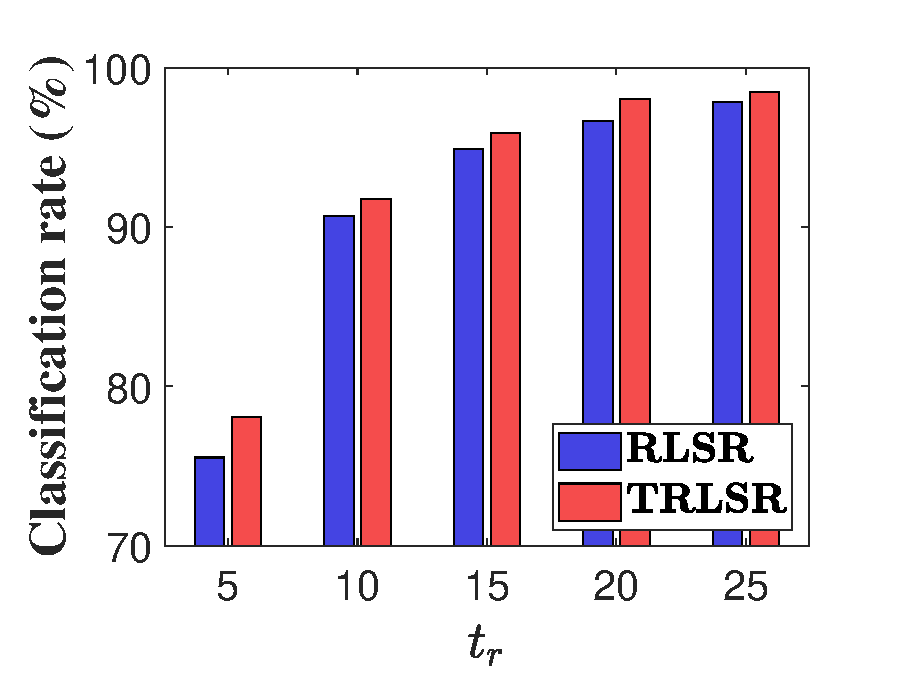
\includegraphics[width=.45\textwidth]{figChap6/Fig_Yale_ablation.eps}} &
   \subfigure[AR data set]{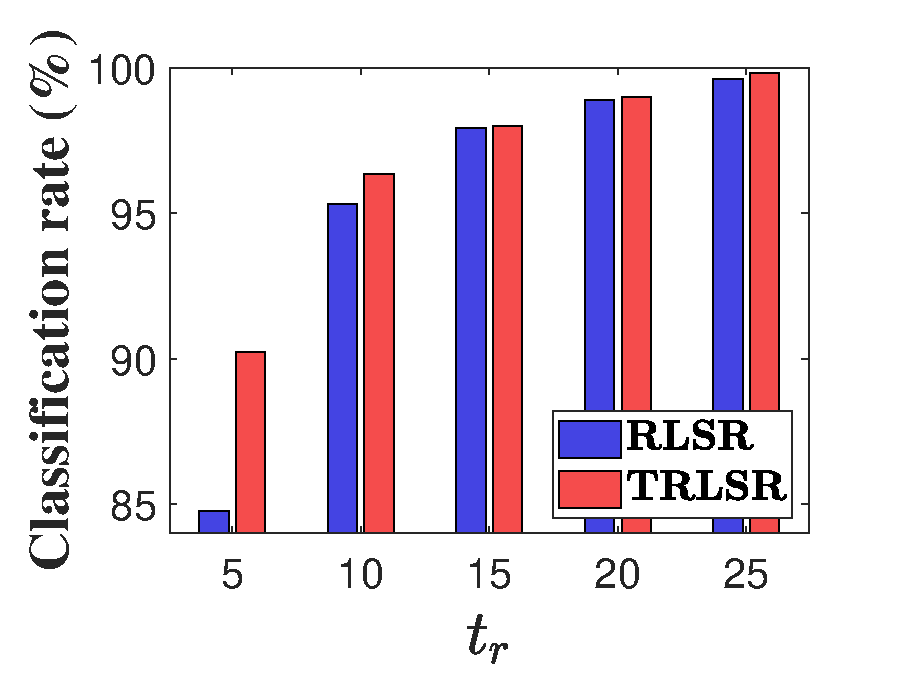
\includegraphics[width=.45\textwidth]{figChap6/Fig_AR_ablation.eps}}\\  
  \subfigure[CMU PIE data set]{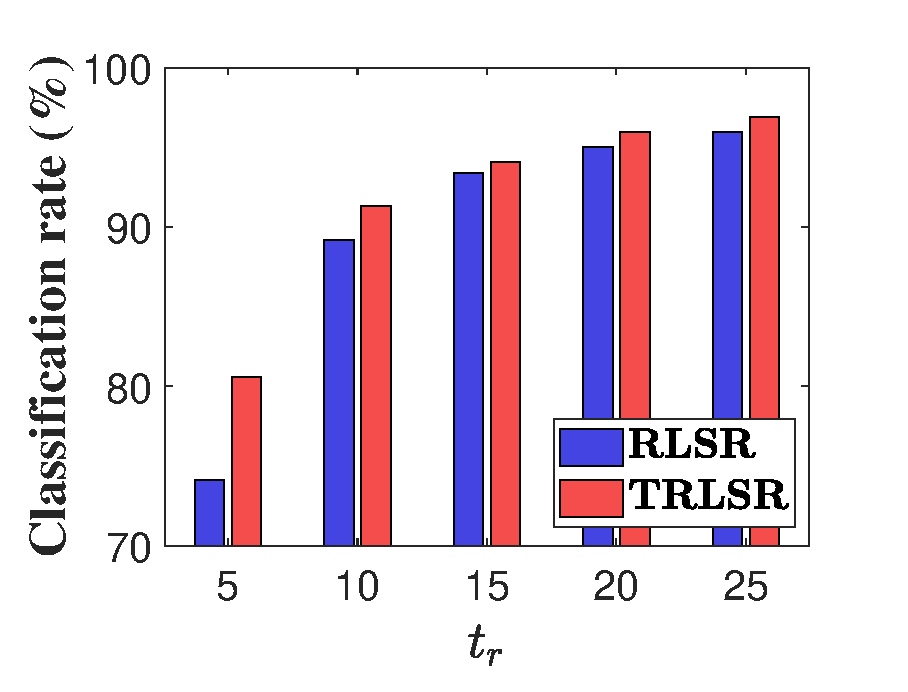
\includegraphics[width=.45\textwidth]{figChap6/Fig_Pie_ablation.eps}} &
 \subfigure[Caltech-101 data set]{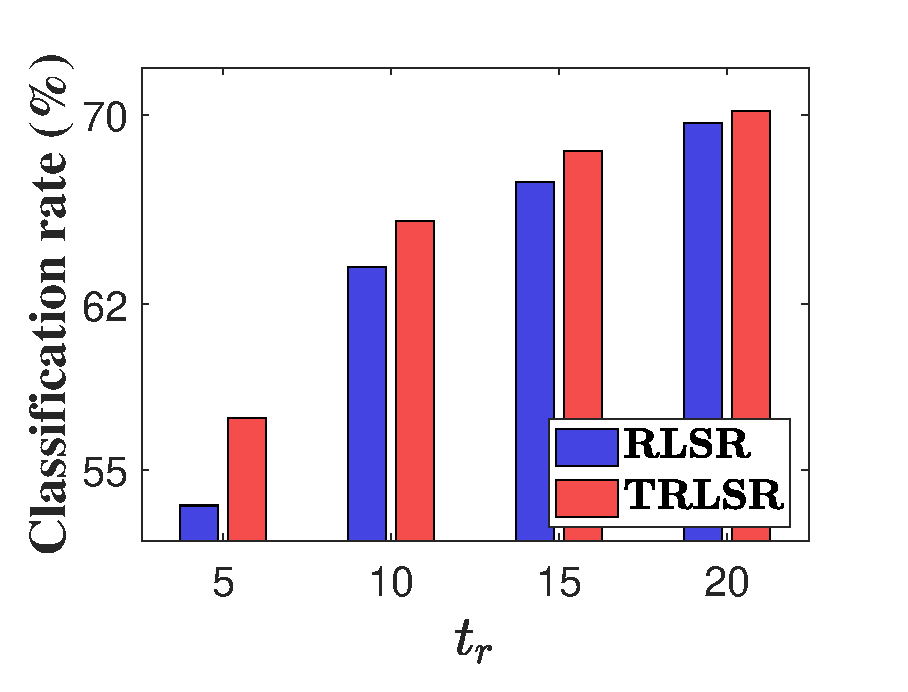
\includegraphics[width=.45\textwidth]{figChap6/Fig_Cal_ablation.eps}}\\
\end{tabular}
\caption{Comparison of the proposed method with and without the twin matrix on different data sets.}
\label{Fig: TRLSR_Ablation_study}
\end{figure}
%-------------------------------------------------------%
%========================================================%
\subsection{Effectiveness of Twin Matrix} 
%
Next, we analyze effectiveness of the twin matrix $\bm{U}$ in the proposed model. Experiments are conducted on the Ex Yale B, AR, CMU PIE, and Caltech-101 data sets, in which the proposed method with and without the twin matrix are compared. The model introduced in~\eqref{eq: TRLSR_OBJ_with_T} can be considered as the proposed TRLSR method reduced to a model without the twin matrix $\bm{U}$. We refer to the model without the twin matrix as the relaxed least squares regression (RLSR). Similar to the earlier experiments, we randomly select the training samples $t_r$ and the remaining samples for testing from the data sets. Each experiment is repeated $10$ times and the mean classification rate is reported.

Fig.~\ref{Fig: TRLSR_Ablation_study} shows the comparison of the TRLSR and RLSR methods on different data sets. It is evident that TRLSR performs better than RLSR, which indicates the effectiveness of the twin matrix. Further, we note that the performance of TRLSR is significantly better than that of RLSR for smaller training numbers on all data sets. This validates the effectiveness of enhanced intra-class similarity using the twin matrix $\bm{U}$ in providing significant gains when the training set size is limited. Overall, this establishes the effectiveness of the proposed regression model in extracting more compact and discriminative features for improved classification performance.
%
%============================================%
\begin{figure}
\centering
 \begin{tabular}{@{}cc@{}}
    \subfigure[Ex Yale B data set]{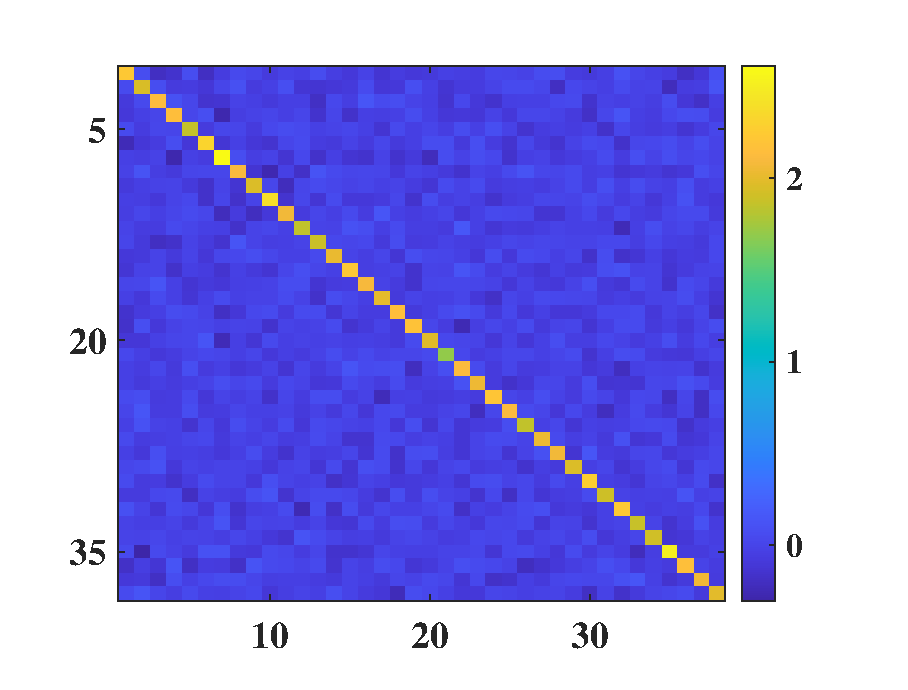
\includegraphics[width=.45\textwidth]{figChap6/PRL_Yale_Vmatrix.eps}} &
   \subfigure[PubFig83 data set]{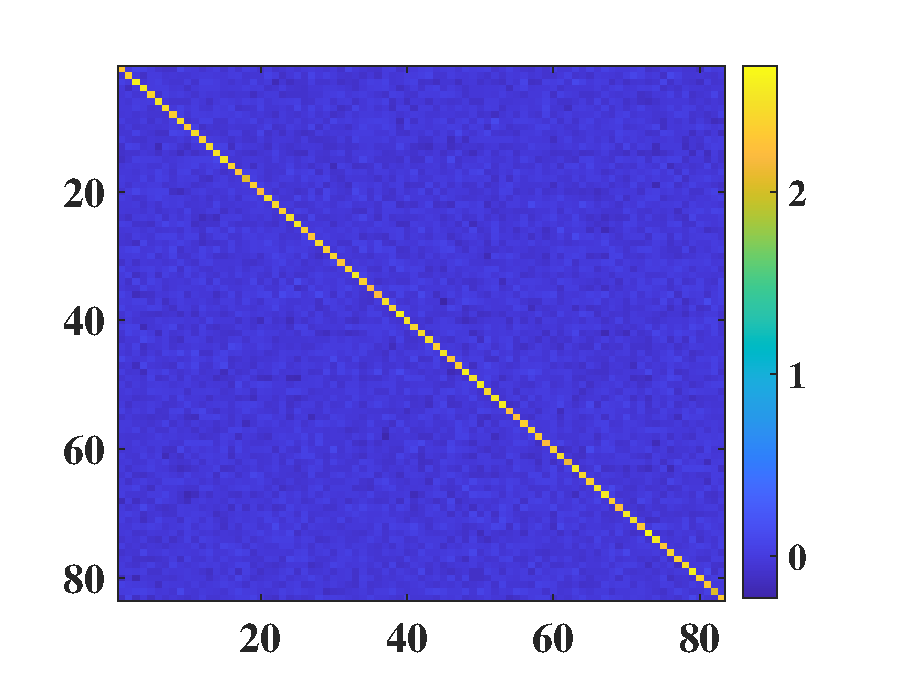
\includegraphics[width=.45\textwidth]{figChap6/PRL_PFG_Vmatrix.eps}}\\  
  \subfigure[CMU PIE data set]{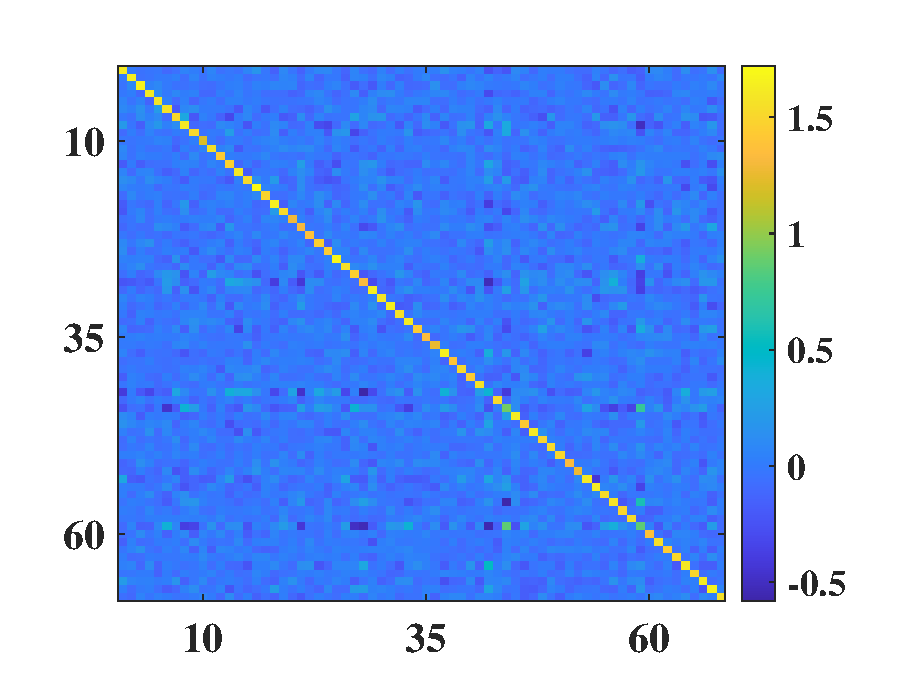
\includegraphics[width=.45\textwidth]{figChap6/PRL_PIE_Vmatrix.eps}} &
 \subfigure[Caltech 101 data set]{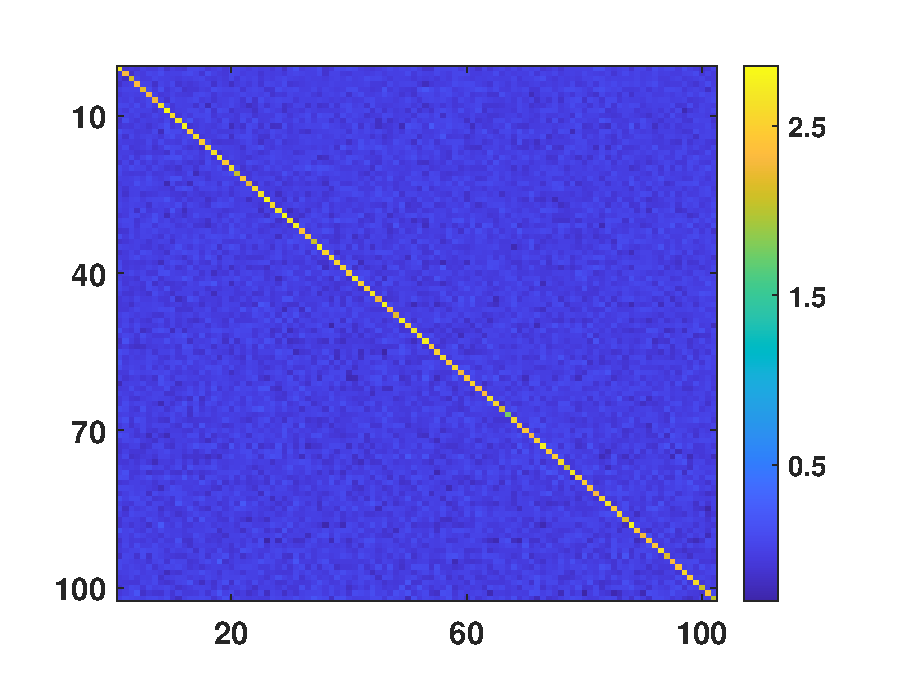
\includegraphics[width=.45\textwidth]{figChap6/PRL_caltech_Vmatrix.eps}}\\
\end{tabular}
\caption{Visualization of the matrix $\bm{V}$ for different data sets.}
\label{Fig: TRLSR_Vmatrix_visulization}
\end{figure}
%======================================================%
%=======================================================%%
\subsection{Significance of Structure Consistency}
%
To ensure structural correspondence between $\bm{T}$ and $\bm{U}$, we introduced a mapping matrix $\bm{V}$. We analyze the matrix $\bm{V}$ to understand the structural similarity between $\bm{T}$ and $\bm{U}$. Fig.~\ref{Fig: TRLSR_Vmatrix_visulization} shows a visualization of matrix $\bm{V}$. It is seen that $\bm{V}$  has a block-diagonal structure which indicates that the samples belonging to the same class in $\bm{T}$ and $\bm{U}$ have some correlation. Due to this structural similarity between $\bm{T}$ and $\bm{U}$, samples belonging to the same class will be close together in the transformed feature space with $\bm{U}$ capturing the intra-class similarity. Note that $\bm{T}$ and $\bm{U}$ are not identical as can be seen from the visualization of $\bm{V}$ as well. Thus, TRLSR allows flexibility in learning projections while enhancing the compactness of the intra-class samples.
%
\subsection{Image Recognition on Large Data Sets using Deep Features}
%
Next, we extract deep features from large data sets in order to evaluate the proposed approach. Deep features can be extracted using different CNN architectures~\cite{VGG,Tatiana}. We consider five large and challenging image data sets: Stanford-40 Actions~\cite{Std_40} for action recognition, Caltech-UCSD Birds data set (CUB-200-2011)~\cite{CUB_2011} for fine-grained object recognition, Caltech-$101$~\cite{Caltech101}, Caltech-$256$, and ImageNet~\cite{Imagenet} data sets for object classification.
%
\subsubsection{Results for Stanford-40 Actions and Caltech-UCSD Birds data sets}
%
Stanford-$40$ Actions data set consists of $9352$ images across $40$ human action classes with each class having $180$-$300$ images. We adopt the training-test split suggested by~\cite{Std_40} and randomly select $100$ images from each class for training and the rest for testing. CUB-200-2011 data set consists of $11,788$ images belonging to $200$ bird categories with varying illumination, pose, and viewpoint. We randomly select $30$ images per class for training. The mean classification rate using VGG~\cite{VGG} deep features are listed in Table~\ref{table: Std_CUB}. It is seen that the proposed approach has improved classification rate on the Stanford-40 Actions data set. On the CUB-200-2011 data set, PRoCRC has $1 \%$ higher classification rate than TRLSR, although TRLSR has better rate than the other methods.
%========================================================%
\begin{table}
\caption{Mean classification rate ($\%$) of TRLSR method for large scale data sets.}
\label{table: Std_CUB}
\centering
\small
\begin{tabular}{|c|c|c|}
\hline
\multirow{2}{*}{\textbf{Algorithm}} & \multicolumn{2}{c|}{Datasets}                            \\ \cline{2-3} 
                                    & \multicolumn{1}{c|}{Stanford-40 Actions} & CUB-200-2011  \\ \hline
SRC                                 & \multicolumn{1}{c|}{78.7}                & 76.0          \\ \hline
CRC                                 & \multicolumn{1}{c|}{78.2}                & 76.2          \\ \hline
ProCRC                              & \multicolumn{1}{c|}{80.9}                & \textbf{81.9}          \\ \hline
DLSR                                & \multicolumn{1}{c|}{80.3}                & 77.3          \\ \hline
ReLSR                               & \multicolumn{1}{c|}{80.9}                & 78.6          \\ \hline
GReLSR                              & \multicolumn{1}{c|}{81.3}                & 78.8          \\ \hline
DRR                                 & \multicolumn{1}{c|}{73.4}                & 79.0          \\ \hline
TRLSR                               & \multicolumn{1}{c|}{\textbf{82.4}}       & 80.1 \\ \hline
\end{tabular}
\end{table}
%==================================================%%
\subsubsection{Results using DeCaf Features for Caltech-101 and Caltech-256 data sets}
%
The Caltech-$256$ data set consists of images with high object location variability. We evaluate the performance of the proposed TRLSR method using the DeCaf-8 features of Caltech-$256$, and DeCaf-6 features of Caltech-$101$~\cite{Tatiana}. For the Caltech-$256$ data set, we randomly select $10$ images from each class for training, and the rest for testing. Similarly, for the Caltech-$101$ data set, we randomly select $10$-$25$ images from each object category for training, and the rest for testing. We repeat this selection process $10$ times and report the mean classification rates in Table~\ref{table: TRLSR_cal_256} and Table~\ref{table: TRLSR_cal_101}. The results show that the proposed TRLSR method achieves the best classification performance.
%
\begin{table}
\caption{Mean classification rate ($\%$) using deep features for Caltech-$256$ data set.}
\label{table: TRLSR_cal_256}
\centering
\begin{tabular}{|c|c|}
\hline
Method & \begin{tabular}[c]{@{}c@{}}Rate (\%)\end{tabular} \\ \hline 
SRC~\cite{SRC}     & 40.3        \\ \hline
SVM~\cite{SVM}     & 38.7         \\ \hline
CRC~\cite{CRC}     & 40.8         \\ \hline
SA-CRC~\cite{SA-CRC}  & 40.1     \\ \hline
LCKSVD~\cite{LCKSVD}  & 38.6     \\ \hline
FDDL~\cite{FDDL}    & 39.2        \\ \hline
LCLE-DL~\cite{LCLE} & 42.2        \\ \hline
LRSDL~\cite{LRSDL}   & 39.3     \\ \hline
DLSR~\cite{DLSR}    & 43.6        \\ \hline
SALPL~\cite{SALPL}   & 42.1   \\ \hline
TRLSR & \textbf{44.8}        \\ \hline
\end{tabular}
\end{table}
%
\begin{table}
\caption{Mean classification rate ($\%$) using deep features for Caltech-$101$ data set.}
\label{table: TRLSR_cal_101}
\centering
\begin{tabular}{|c|c|c|c|c|}
\hline
\multirow{2}{*}{Method} & \multicolumn{4}{c|}{Training number ($t_r$)}\\ 
\cline{2-5} 
& \multicolumn{1}{c|}{10}             & \multicolumn{1}{c|}{15}             & \multicolumn{1}{c|}{20}             & 25             \\ \hline 
LRC~\cite{LRC}                        & \multicolumn{1}{c|}{75.84}          & \multicolumn{1}{c|}{78.17}          & \multicolumn{1}{c|}{78.89}          & 79.22          \\ \hline
CRC~\cite{CRC}                        & \multicolumn{1}{c|}{76.61}          & \multicolumn{1}{c|}{79.11}          & \multicolumn{1}{c|}{79.97}          & 80.63          \\ \hline
LRRR~\cite{LRLR_SLRR}                       & \multicolumn{1}{c|}{74.62}          & \multicolumn{1}{c|}{76.67}          & \multicolumn{1}{c|}{78.38}          & 79.34          \\ \hline
SLRR~\cite{LRLR_SLRR}                       & \multicolumn{1}{c|}{74.71}          & \multicolumn{1}{c|}{78.46}          & \multicolumn{1}{c|}{80.58}          & 82.46          \\ \hline
DLSR~\cite{DLSR}                       & \multicolumn{1}{c|}{78.65}          & \multicolumn{1}{c|}{80.29}          & \multicolumn{1}{c|}{81.28}          & 81.64          \\ \hline
ReLSR~\cite{ReLSR}                      & \multicolumn{1}{c|}{79.48}          & \multicolumn{1}{c|}{81.26}          & \multicolumn{1}{c|}{82.17}          & 82.47          \\ \hline
RLSL~\cite{RLSL}                       & \multicolumn{1}{c|}{79.17}          & \multicolumn{1}{c|}{81.39}          & \multicolumn{1}{c|}{82.54}          & 83.06          \\ \hline
RDR~\cite{RDR}                        & \multicolumn{1}{c|}{80.12}          & \multicolumn{1}{c|}{81.32}          & \multicolumn{1}{c|}{82.14}          & 82.46          \\ \hline
RSLDA~\cite{RSLDA}                      & \multicolumn{1}{c|}{74.36}          & \multicolumn{1}{c|}{76.30}          & \multicolumn{1}{c|}{77.43}          & 78.35          \\ \hline
ICS\_DLSR~\cite{ICS_DLSR}                  & \multicolumn{1}{c|}{79.53}          & \multicolumn{1}{c|}{82.07}          & \multicolumn{1}{c|}{82.96}          & 83.19          \\ \hline
TRLSR                      & \multicolumn{1}{c|}{\textbf{80.94}} & \multicolumn{1}{c|}{\textbf{82.78}} & \multicolumn{1}{c|}{\textbf{82.97}} & \textbf{83.85} \\ \hline
\end{tabular}
\end{table}
%
\subsubsection{Results for ImageNet Data Set}
%
Next, we evaluate the performance of the proposed TRLSR method on the ImageNet data set. ImageNet data set consists of over $1000$ object classes with images of different resolutions and dimensions. Following~\cite{Tatiana}, a subset of the ImageNet (DeCaf-7) data set is used and from this we randomly select $73,244$ images and $52$ classes for our experiment. We select $5$-$25$ images per object class for training and the rest for testing. For each train-test split, we repeat the experiment $10$ times and the mean classification rates are shown in Fig.~\ref{fig: ImageNet_figures}. It is seen that the proposed TRLSR method outperforms the state-of-the-art algorithms while being able to work with a wide range of features.
%
\begin{figure}
\centering
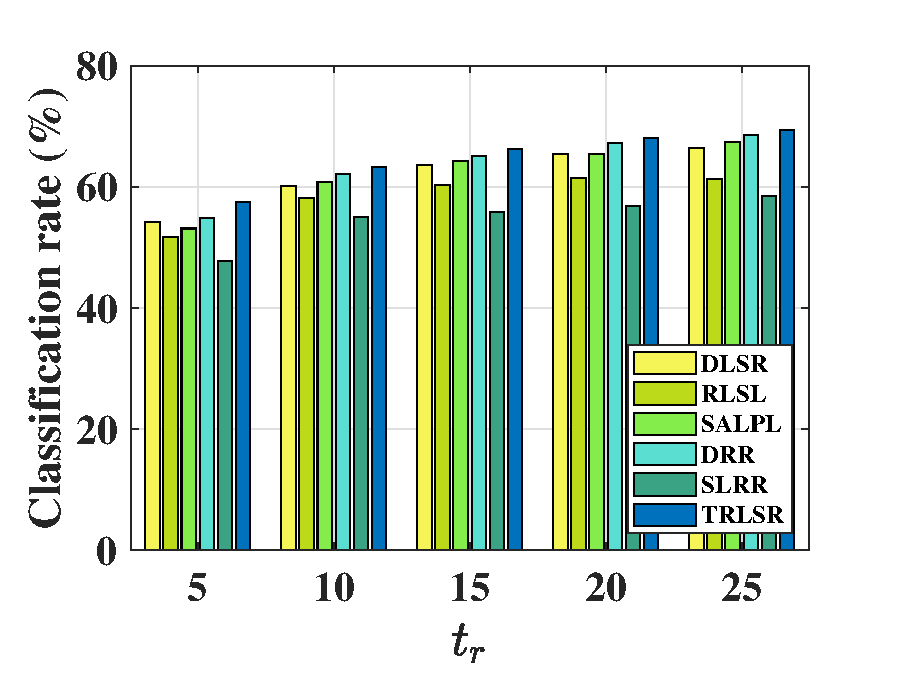
\includegraphics[keepaspectratio,width=0.70\textwidth,trim=0 0 0 0,clip]{figChap6/Fig_imagenet_train.eps}
\caption{Mean classification rate using deep features for the ImageNet data set.}
\label{fig: ImageNet_figures}
\end{figure}
%
\section{TRLSR Model Analysis}
\label{sec: Model}
%
In this section, we consider further analysis of the proposed TRLSR model and algorithm in terms of comparison with deep learning methods, parameter sensitivity, computational complexity, and convergence.
%
\subsection{Comparison with Deep Learning}
%
In recent times, deep neural networks have been able to achieve significant improvement in performance for classification problems, especially with large data sets, than the conventional methods. This indicates that the deep learning methods can extract more discriminative features than the conventional feature extraction methods. However, deep learning methods are data-intensive i.e., they do not generalize well for small data sets and in the presence of large intra-class variability. In such cases, the classification performance of deep learning approaches is expected to degrade significantly~\cite{DFEDL,Homa_object,Few}. We compare the classification performance of deep learning methods with the proposed TRLSR method on the original Ex Yale B data set. In this experiment, we utilize the VGG-16~\cite{VGG} and ResNet-50~\cite{Resnet50} CNN architectures. These architectures are used for feature extraction using pre-trained weights, obtained by training on the ImageNet data set, followed by retraining the weights of the classification layers (dense layers). We also report the classification rate for VGG-16 with trainable weights (VGG-$16^{\ast}$), learning the weights for the feature extraction as well as classification layers. We randomly select $380$ images ($10$ images per class) for training and $2048$ images for testing.

The mean classification rate over $10$ experiment runs is reported in Table~\ref{table: comp_CNN}. It is seen that the proposed TRLSR method significantly outperforms the deep learning approaches. This shows that the performance of the deep learning-based approaches will degrade with limited data sets and fewer training samples~\cite{DFEDL,Homa_object}. For instance, in many real-life applications the true positive cases are rare (cancer detection, defective products in an assembly line, etc.). Additionally, the proposed TRLSR method extracts a compact intra-class structure due to the classwise mean constraint together with the relaxed target in order to exploit inter-class margins. In this way, the transformed features' intra-class structure can be enhanced to achieve superior classification performance. Hence, the proposed feature extraction method improves classification performance even with a limited data set, fewer training numbers, and with images captured in uncontrolled environments.
%
\begin{table}
\caption{Mean classification rate ($\%$) of deep learning methods on Ex Yale B data set.}
\label{table: comp_CNN}
\centering
\begin{tabular}{|c|c|}
\hline
Algorithm & \begin{tabular}[c]{@{}c@{}}Rate (\%)\end{tabular}\\ 
\hline
VGG-16~\cite{VGG} & 55.94\\ \hline
VGG-$16^{\ast}$ & 50.45\\ \hline
ResNet-50~\cite{Resnet50} & 50.63\\ \hline
TRLSR & \textbf{92.07}\\ \hline
\end{tabular}
\end{table}
%
%=======================================%%
%==========================================================%
\begin{figure}
\centering
\begin{tabular}{@{}cc@{}}
\subfigure[Ex Yale B data set\label{fig: yale_tau}]{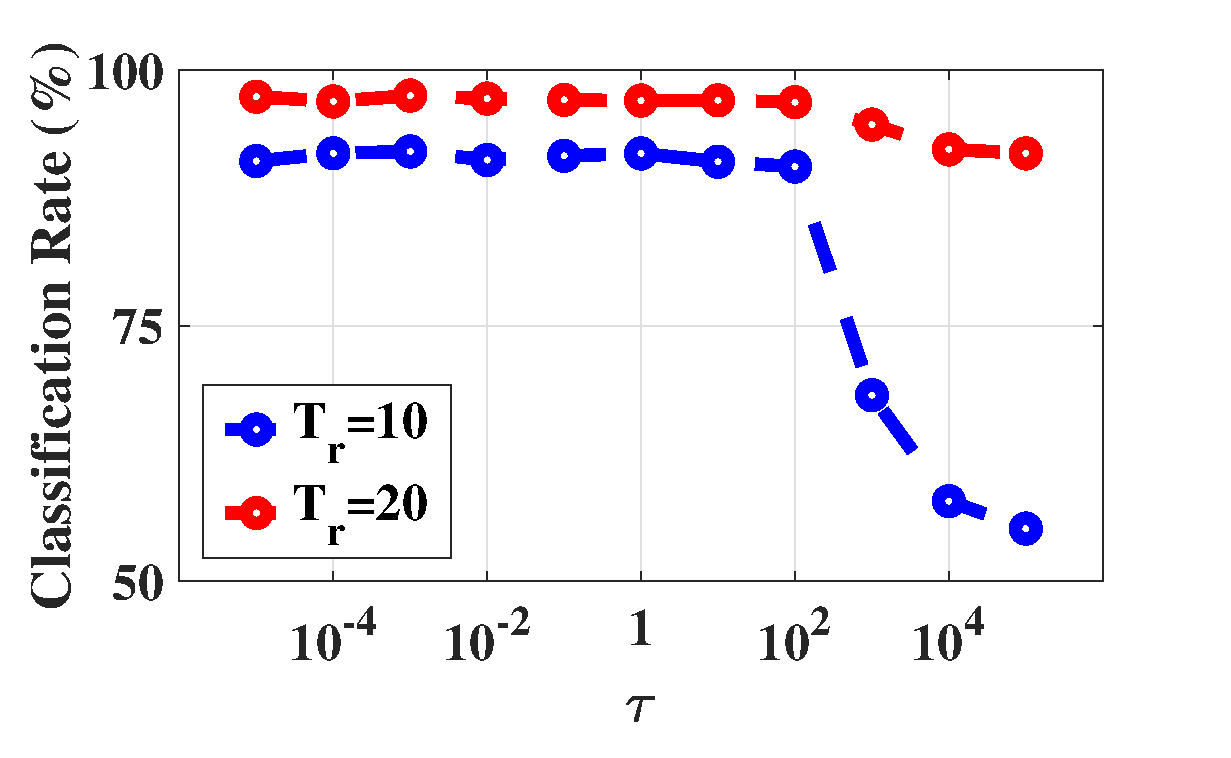
\includegraphics[width=.45\textwidth]{figChap6/PRL_yale_rate_tau.eps}} &
\subfigure[PubFig83 data set\label{fig: pfg_tau}]{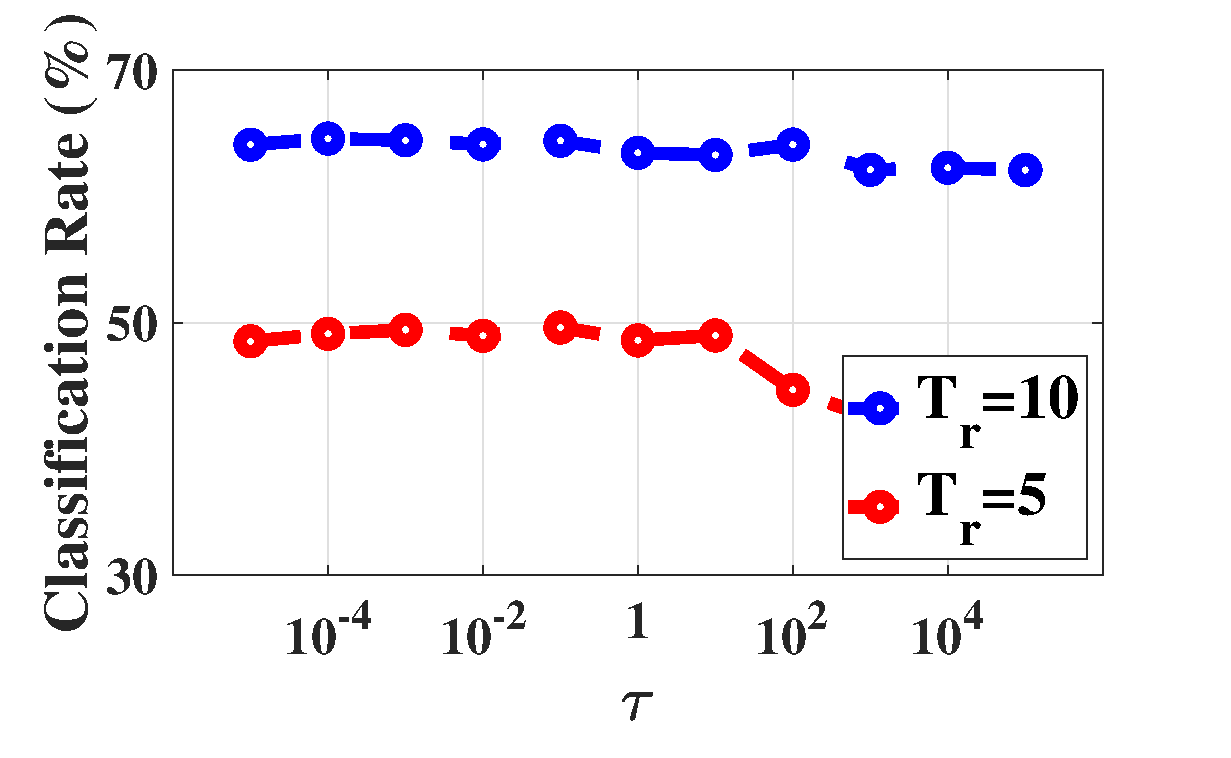
\includegraphics[width=.45\textwidth]{figChap6/PRL_pubfig_rate_tau.eps}}\\
\subfigure[AR data set\label{fig: AR_tau}]{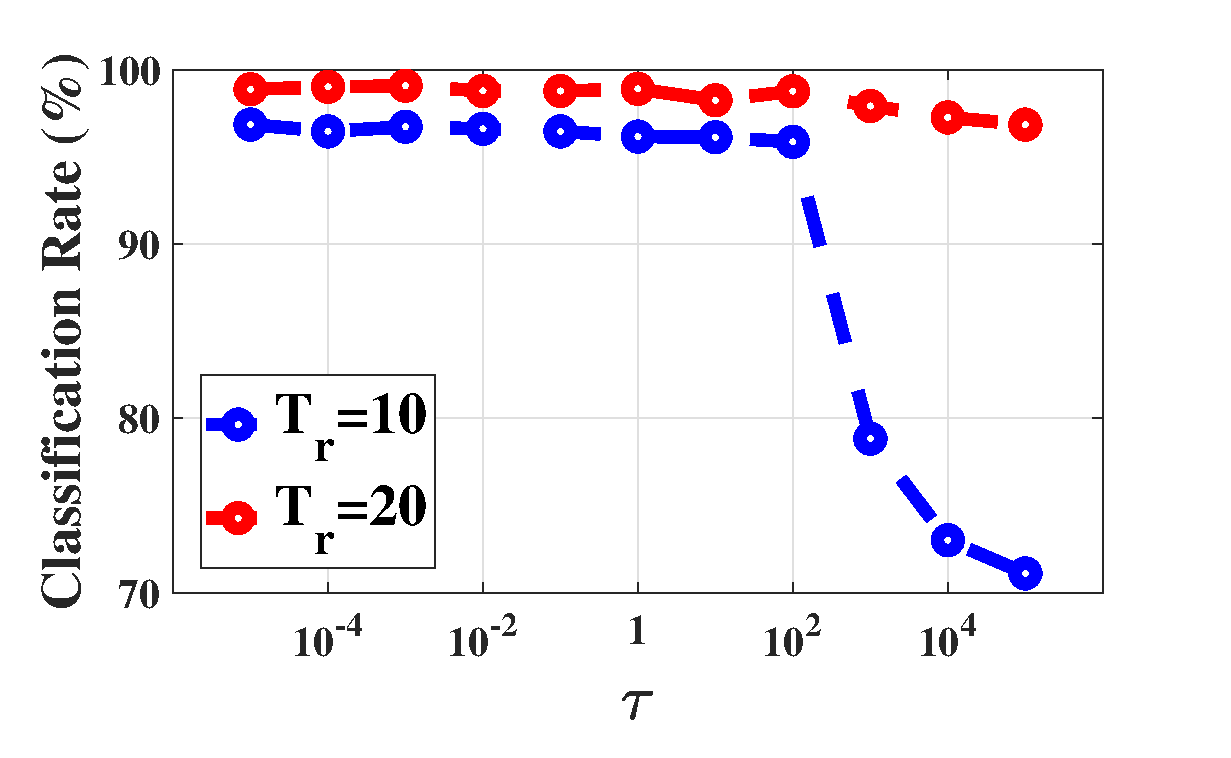
\includegraphics[width=.45\textwidth]{figChap6/PRL_AR_rate_tau.eps}} &
\subfigure[15-Scene data set\label{fig: scene_tau}]{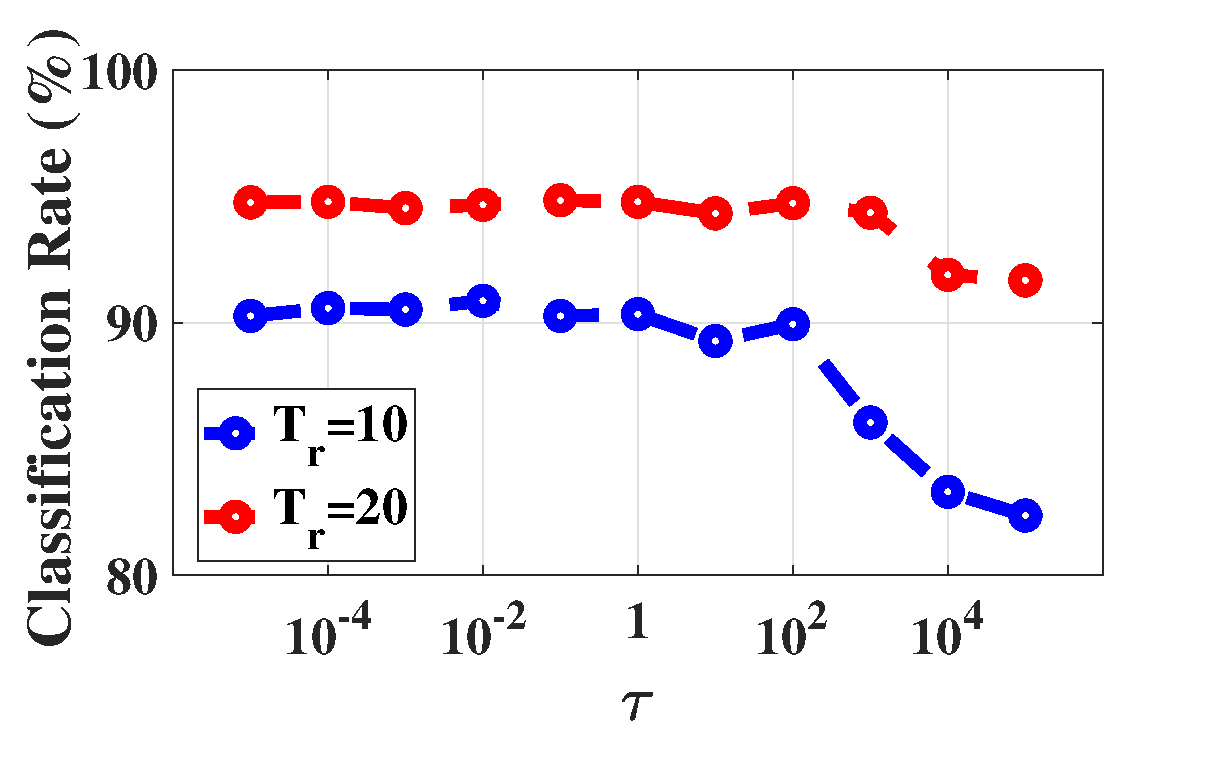
\includegraphics[width=.45\textwidth]{figChap6/PRL_scene_rate_tau.eps}} \\
\subfigure[PubFig83 data set\label{fig: PRL_PFG_alpha}]{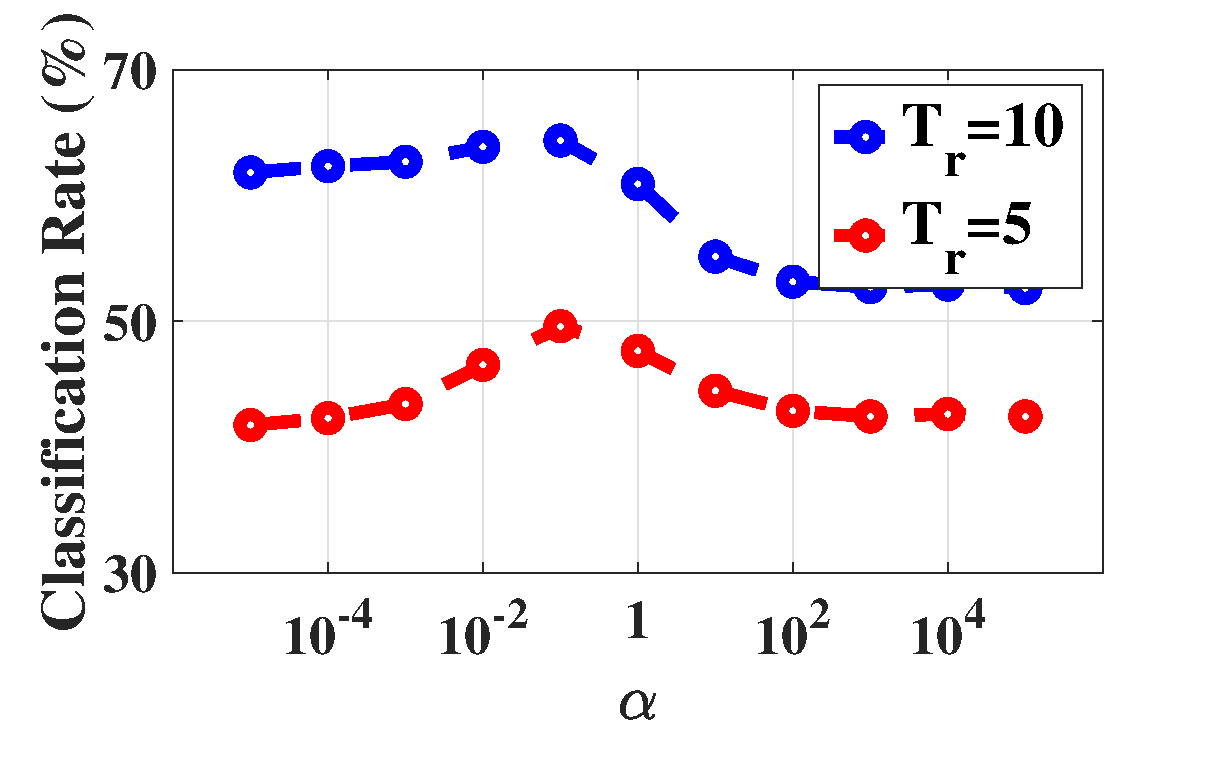
\includegraphics[width=.45\textwidth]{figChap6/PRL_pubfig_rate_alpha.eps}} &
\subfigure[Caltech-101 data set\label{fig: cal_alpha}]{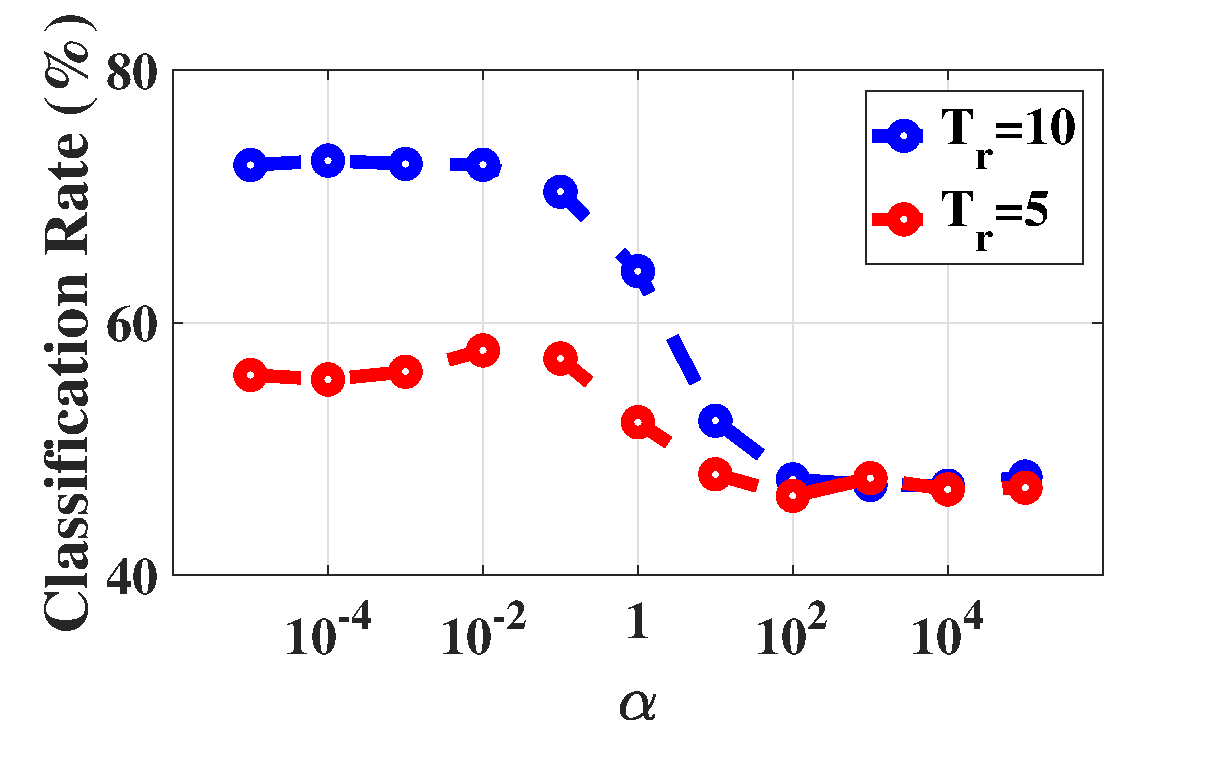
\includegraphics[width=.45\textwidth]{figChap6/Fig_PRL_caltech_rate_alpha.eps}} \\
\subfigure[AR data set\label{fig: AR_alpha}]{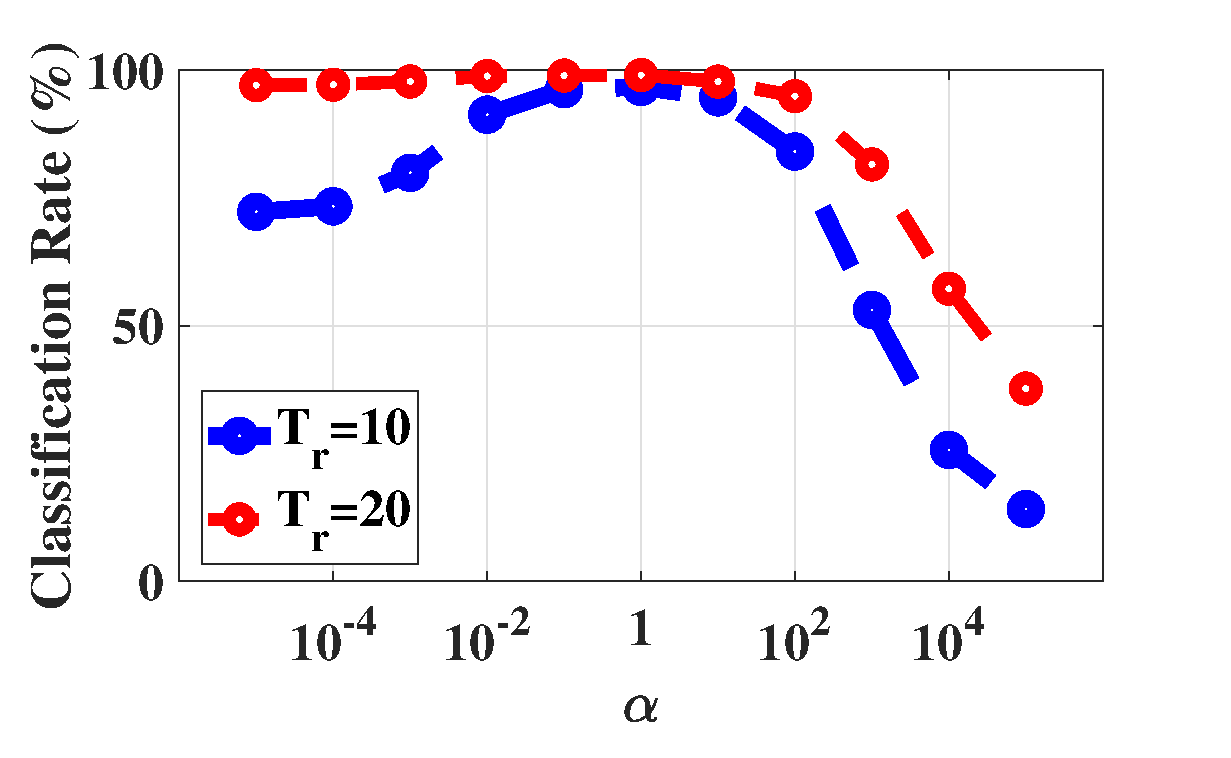
\includegraphics[width=.45\textwidth]{figChap6/PRL_AR_rate_alpha.eps}} &
\subfigure[Ex Yale B data set\label{fig: Yale_alpha}]{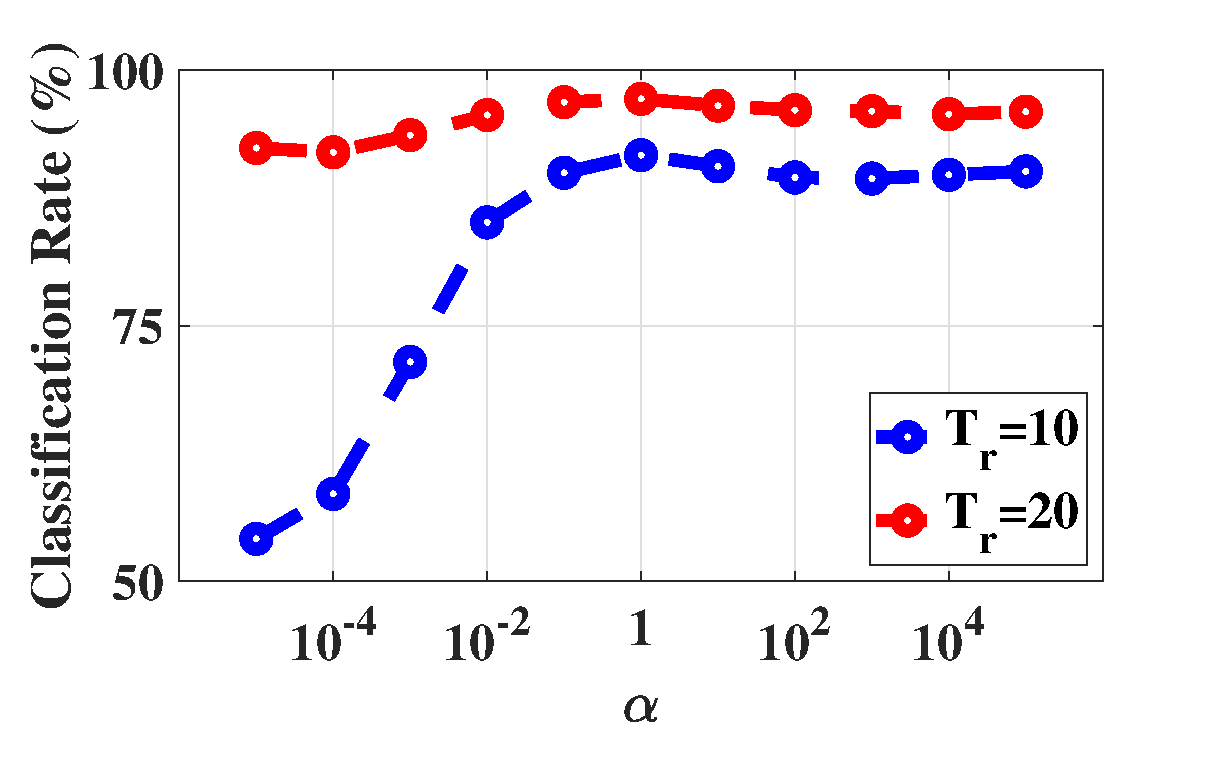
\includegraphics[width=.45\textwidth]{figChap6/PRL_yale_rate_alpha.eps}} 
\end{tabular}
\caption{Mean classification rate ($\%$) of the proposed TRLSR method as a function of the weight parameter $\gamma$  and $\tau$ on different data sets}
\label{Fig: TRLSR_Rate_alpha_tau}
\end{figure}
%===================================%
\begin{figure}
\centering
\subfigure[AR data set]{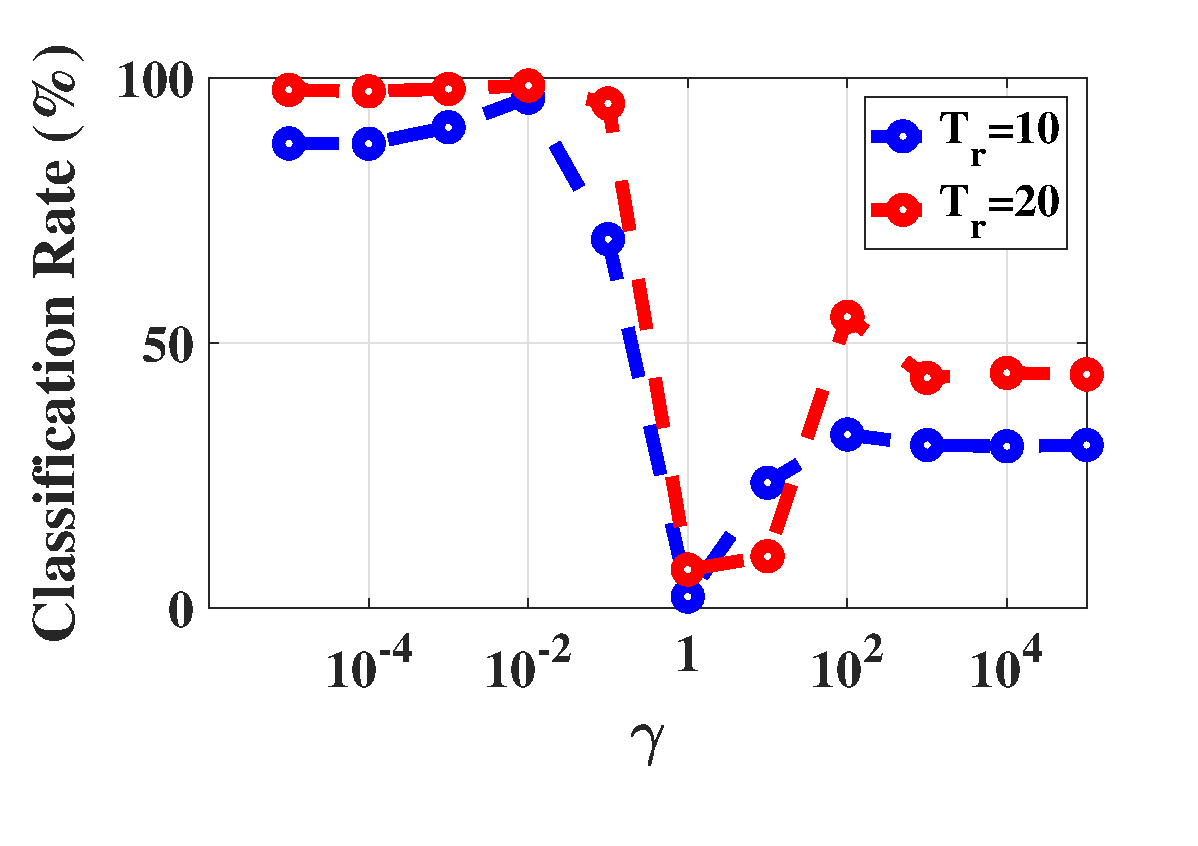
\includegraphics[keepaspectratio,width=0.45\textwidth]{figChap6/Fig_PRL_AR_gamma.eps}} 
\subfigure[Ex Yale B data set]{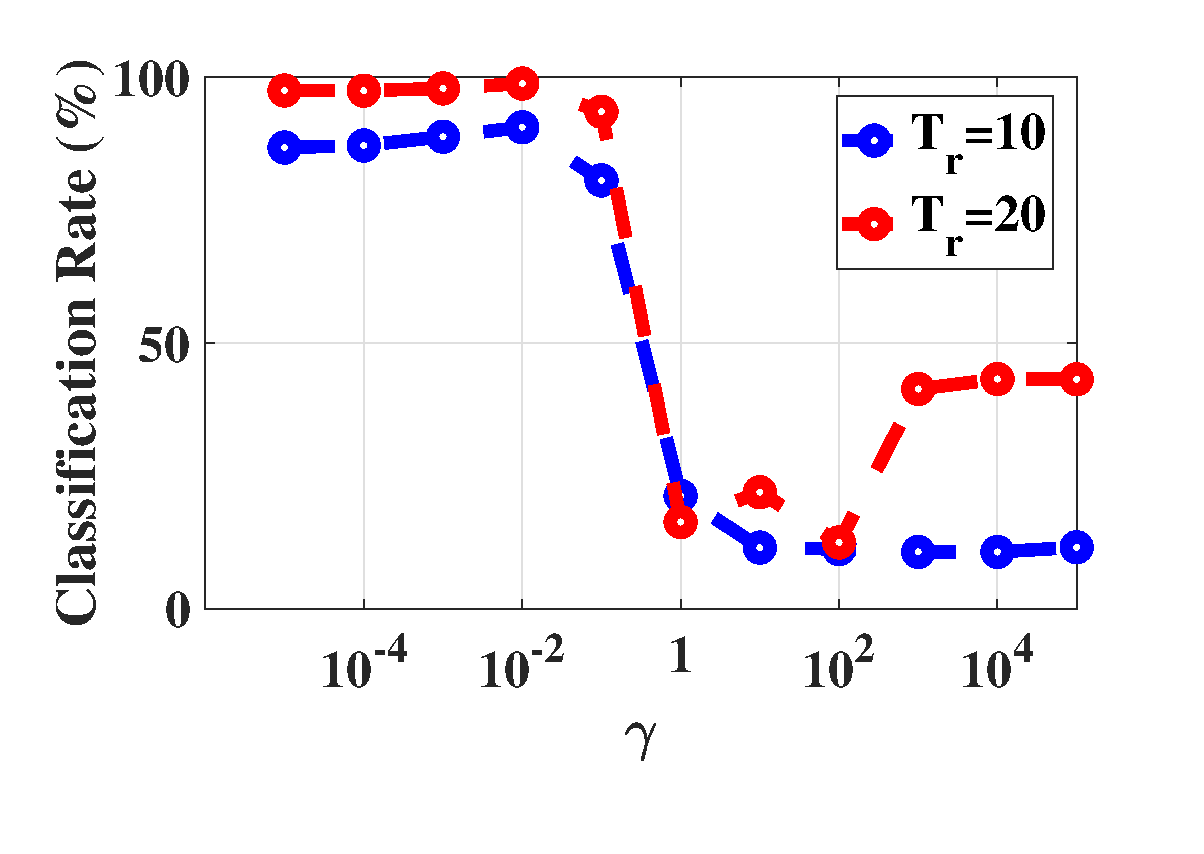
\includegraphics[keepaspectratio,width=0.45\textwidth]{figChap6/Fig_PRL_yale_gamma.eps}}
\caption{Mean classification rate ($\%$) of the proposed TRLSR method as a function of the weight parameter $\gamma$ on different data sets.}
\label{Fig: TRLSR_rate_gamma}
%\vspace{-0.2cm}
\end{figure}
%=====================================================%
%%============================================================%%
\subsection{Parameter Selection}
%
In the proposed TRLSR method, there are three weight parameters $\alpha$, $\gamma$, and $\tau$ which determine the relative importance of the different terms. We tune these parameters over the interval $\left[ 1\mathrm{e}{-5},1\mathrm{e}{5} \right]$. The classification rate of TRLSR as a function of these parameters on different data sets are shown in Fig.~\ref{Fig: TRLSR_Rate_alpha_tau}, Fig.~\ref{Fig: TRLSR_rate_gamma} and Fig~\ref{fig: TRLSR_alpha_tau}. It is observed that TRLSR achieves best performance when $\gamma < 0.1$. Further, the best classification rate can be achieved when $\alpha \in \left[ 1\mathrm{e}{-1}, 1\mathrm{e}{1} \right]$ and it degrades rapidly when $\alpha < 1\mathrm{e}{-1}$. The best classification rate on PubFig83 and 15-Scene data sets are achieved when $\alpha = 1\mathrm{e}{-1}$ as seen from Fig.~\ref{fig: PRL_PFG_alpha} and Fig.~\ref{fig: cal_alpha}, respectively. This indicates that matrix $\bm{U}$ by focusing on maximizing the intra-class similarity aids in extracting more discriminative features. Similarly, TRLSR achieves best classification performance on most data sets considered here with $\tau < 1\mathrm{e}{2}$. These results show that the proposed TRLSR method is fairly robust to the value of the weight parameters while achieving compact and discriminative features.
%===================================================================%
\begin{figure}
\centering
\begin{tabular}{@{}cc@{}}
    \subfigure[AR data set]{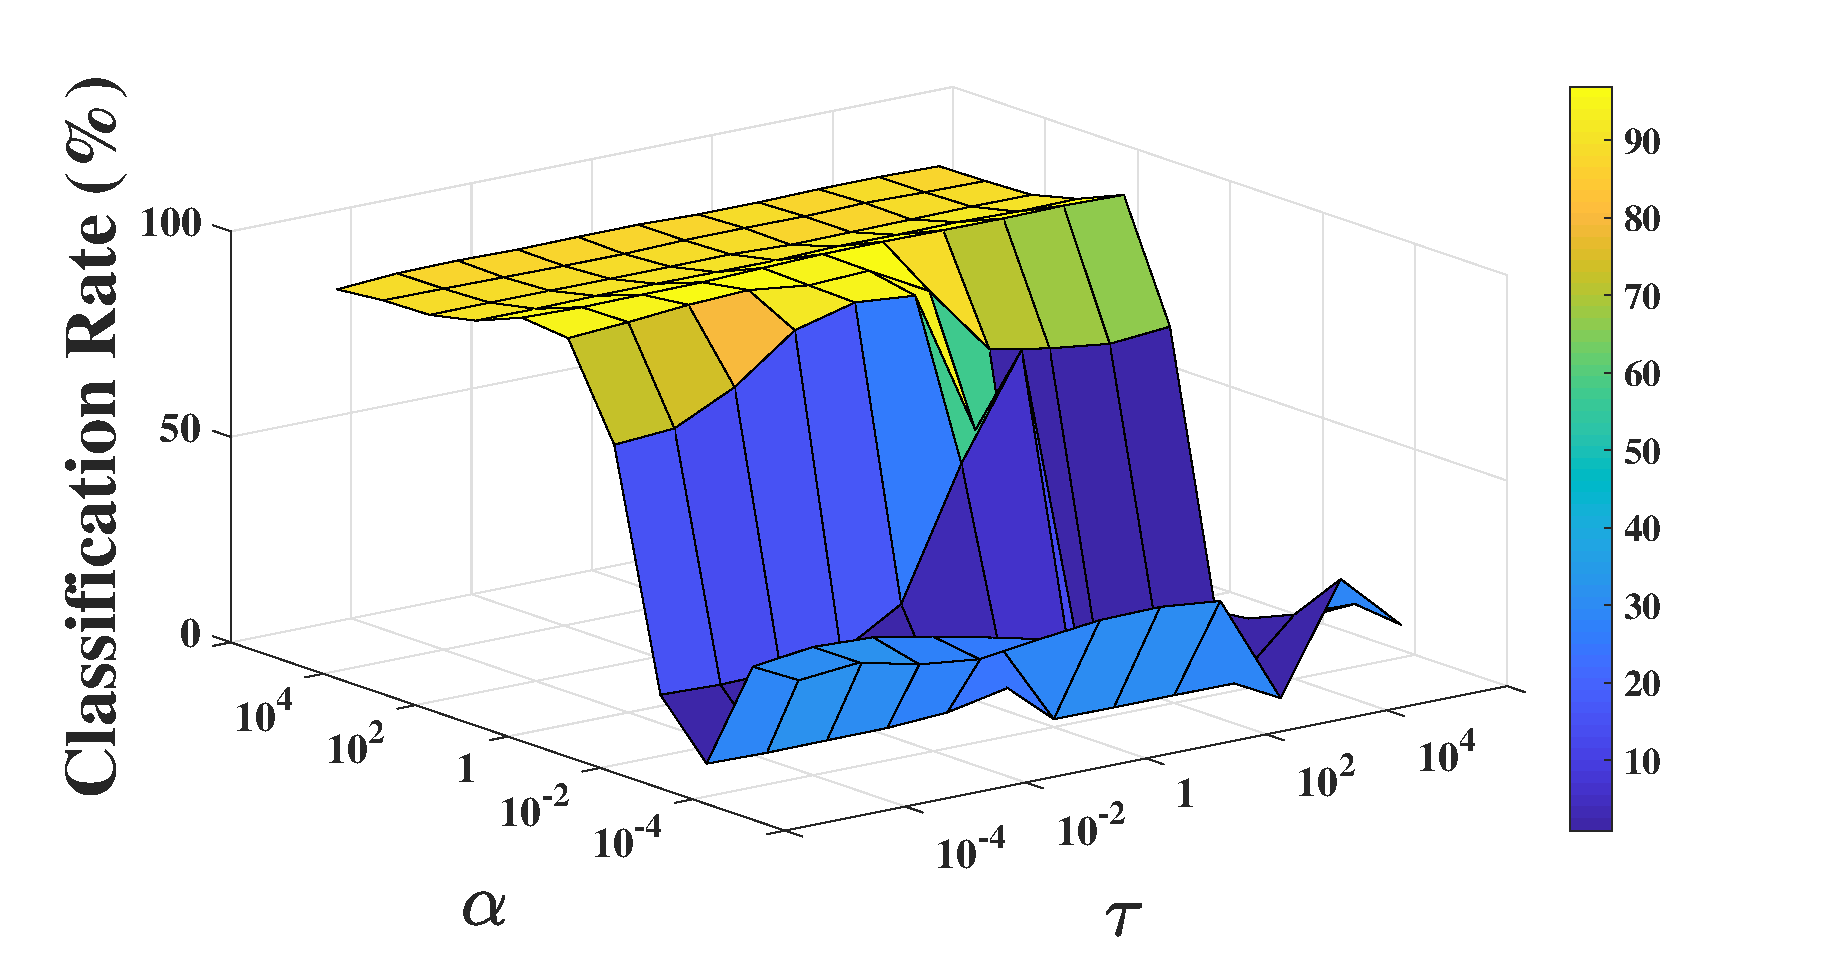
\includegraphics[width=.45\textwidth]{figChap6/Fig_AR_rate_alpha_tau.eps}} &
    \subfigure[Caltech-$101$ data set]{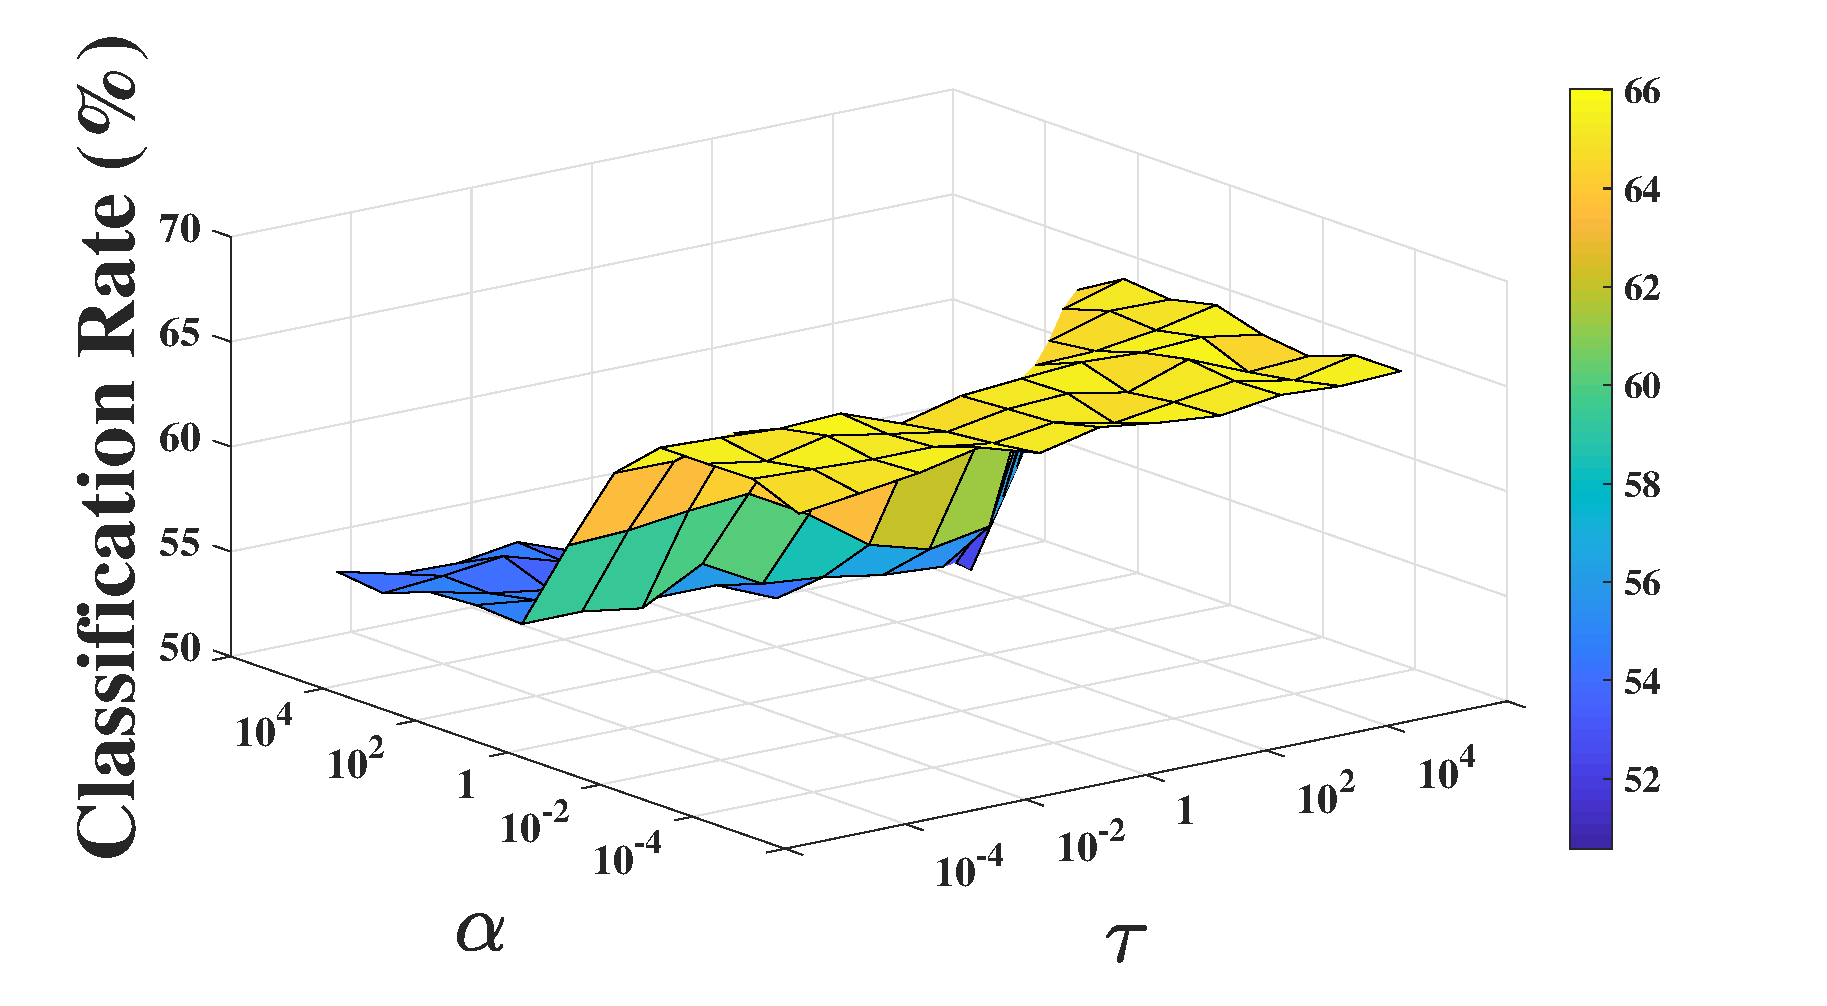
\includegraphics[width=.45\textwidth]{figChap6/Fig_caltech_rate_alpha_tau.eps}}\\  
    \subfigure[Ex Yale B data set ]{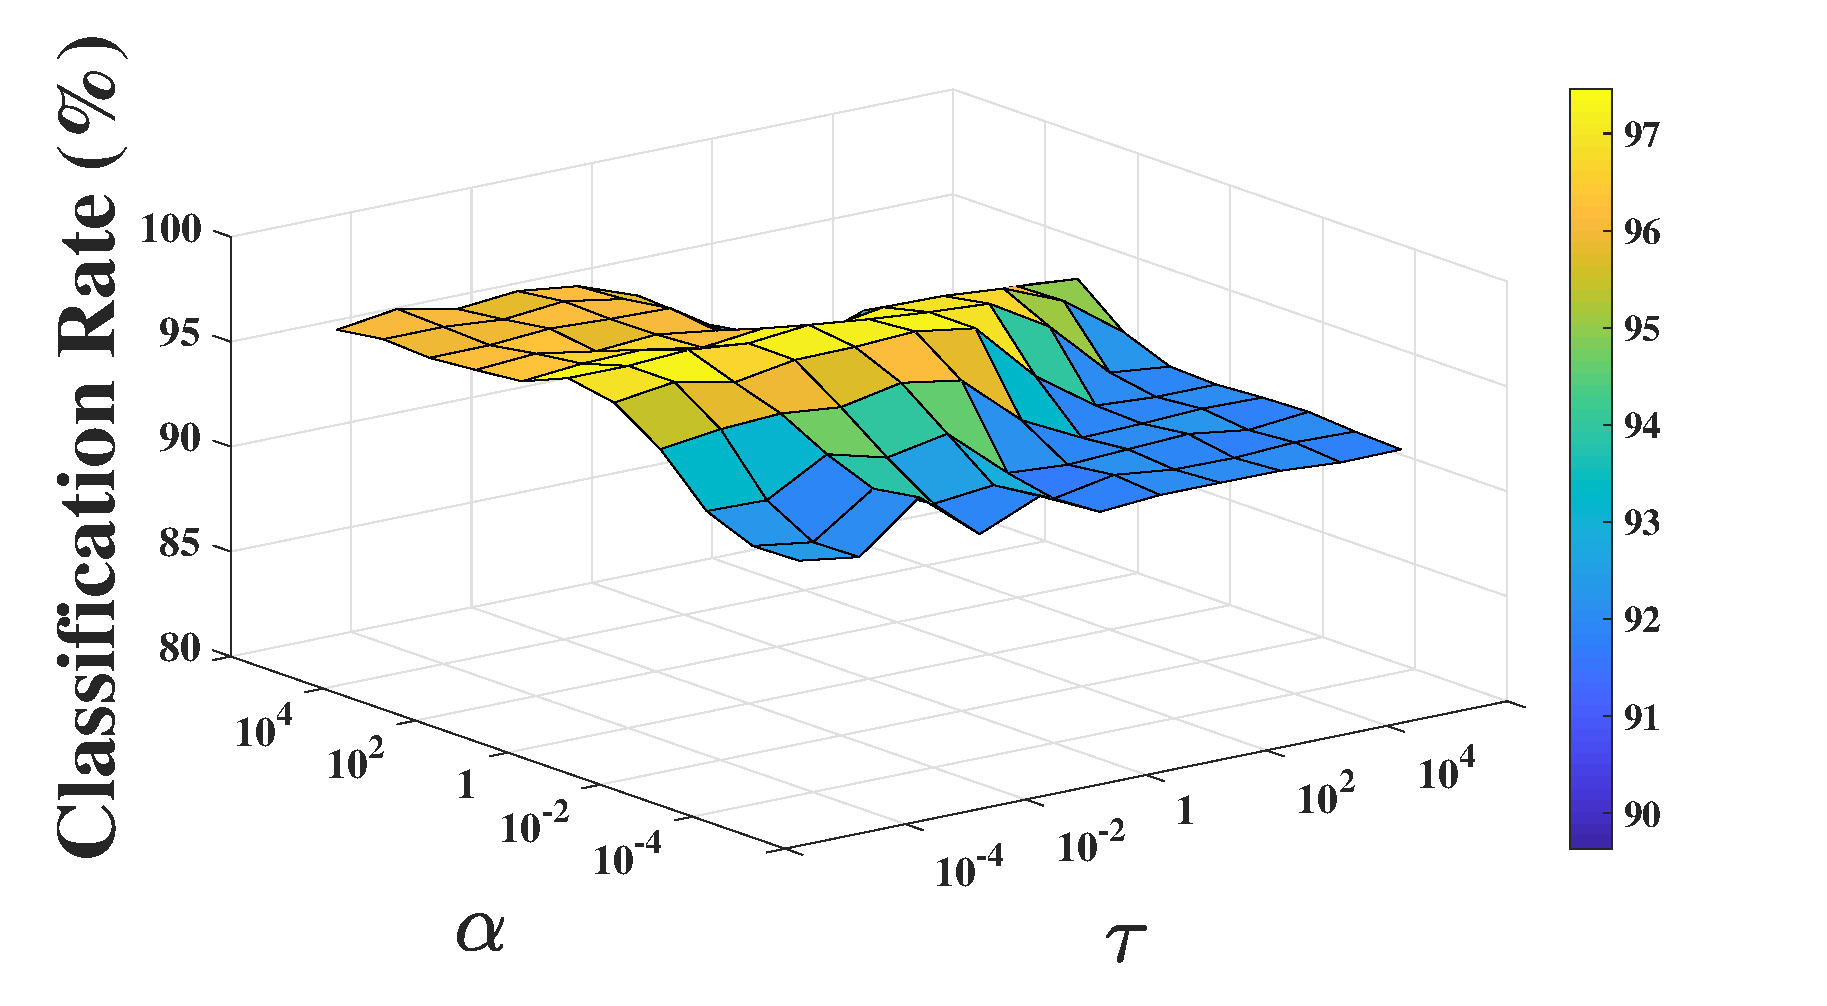
\includegraphics[width=.45\textwidth]{figChap6/Fig_yale_alpha_tau.eps}} &
    \subfigure[15-Scene data set]{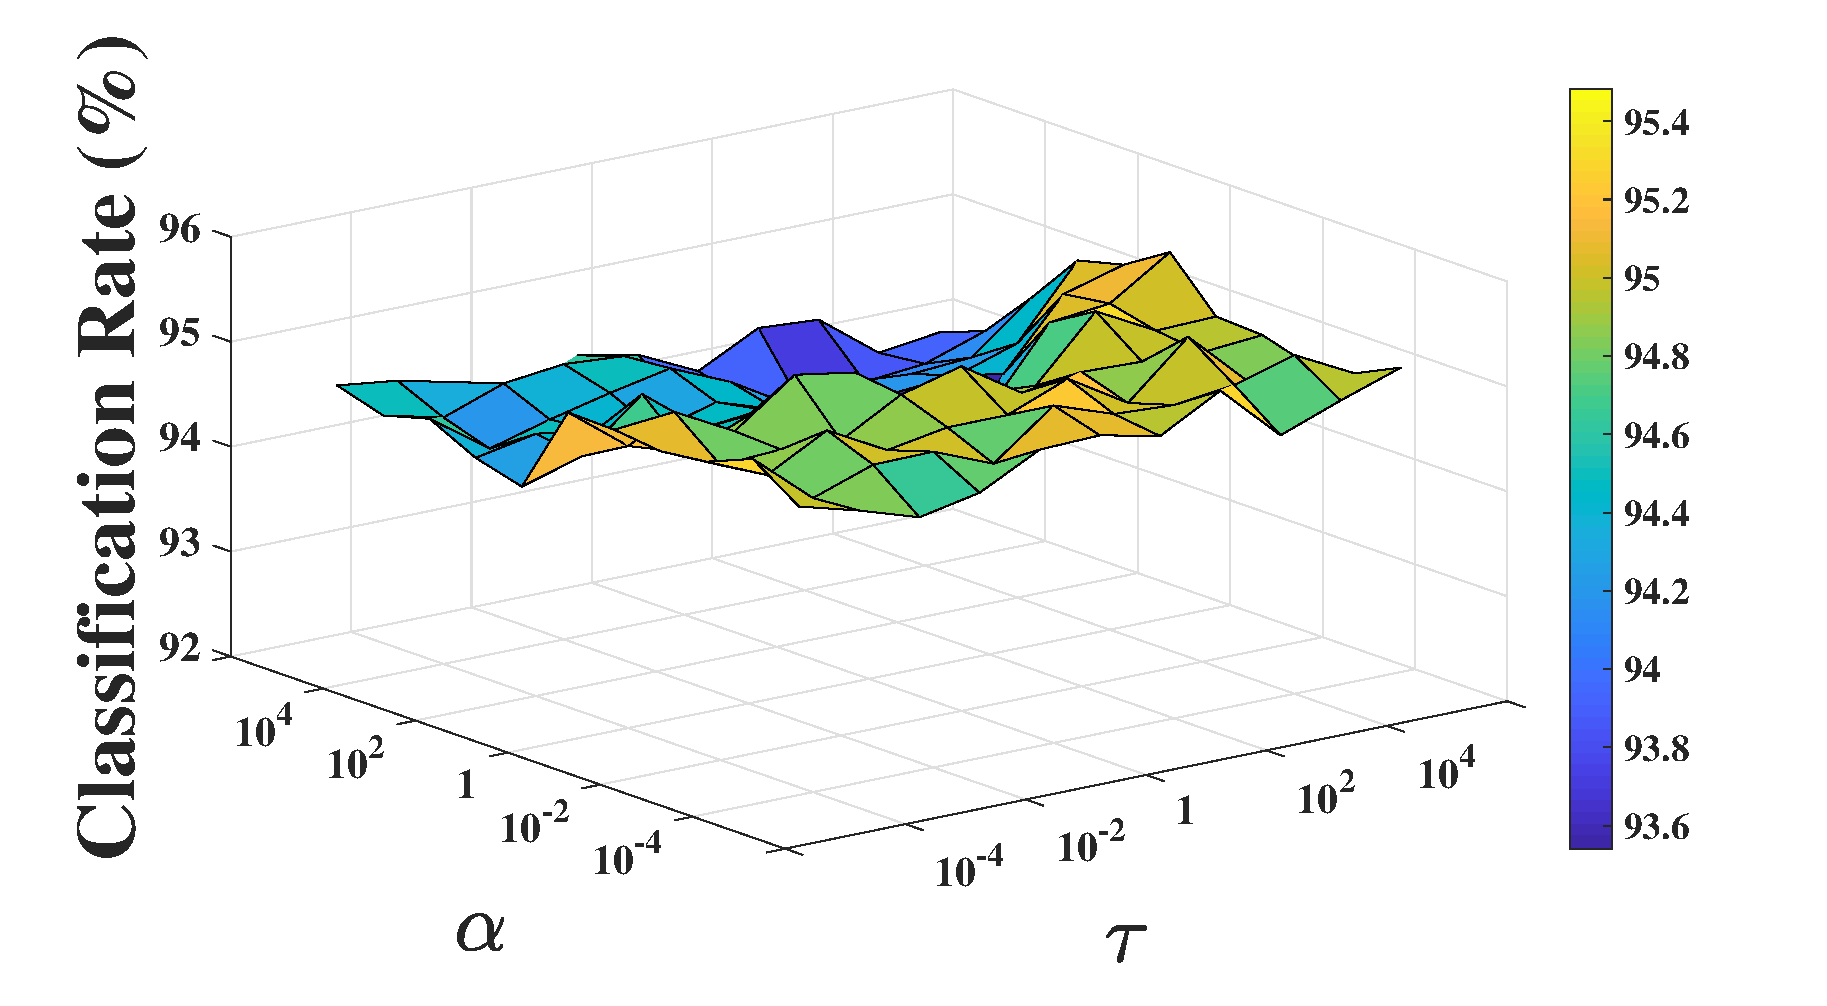
\includegraphics[width=.45\textwidth]{figChap6/Fig_scene_alpha_tau.eps}} \\
    \subfigure[PubFig83 data set]{\label{fig:PFG_alpha_tau}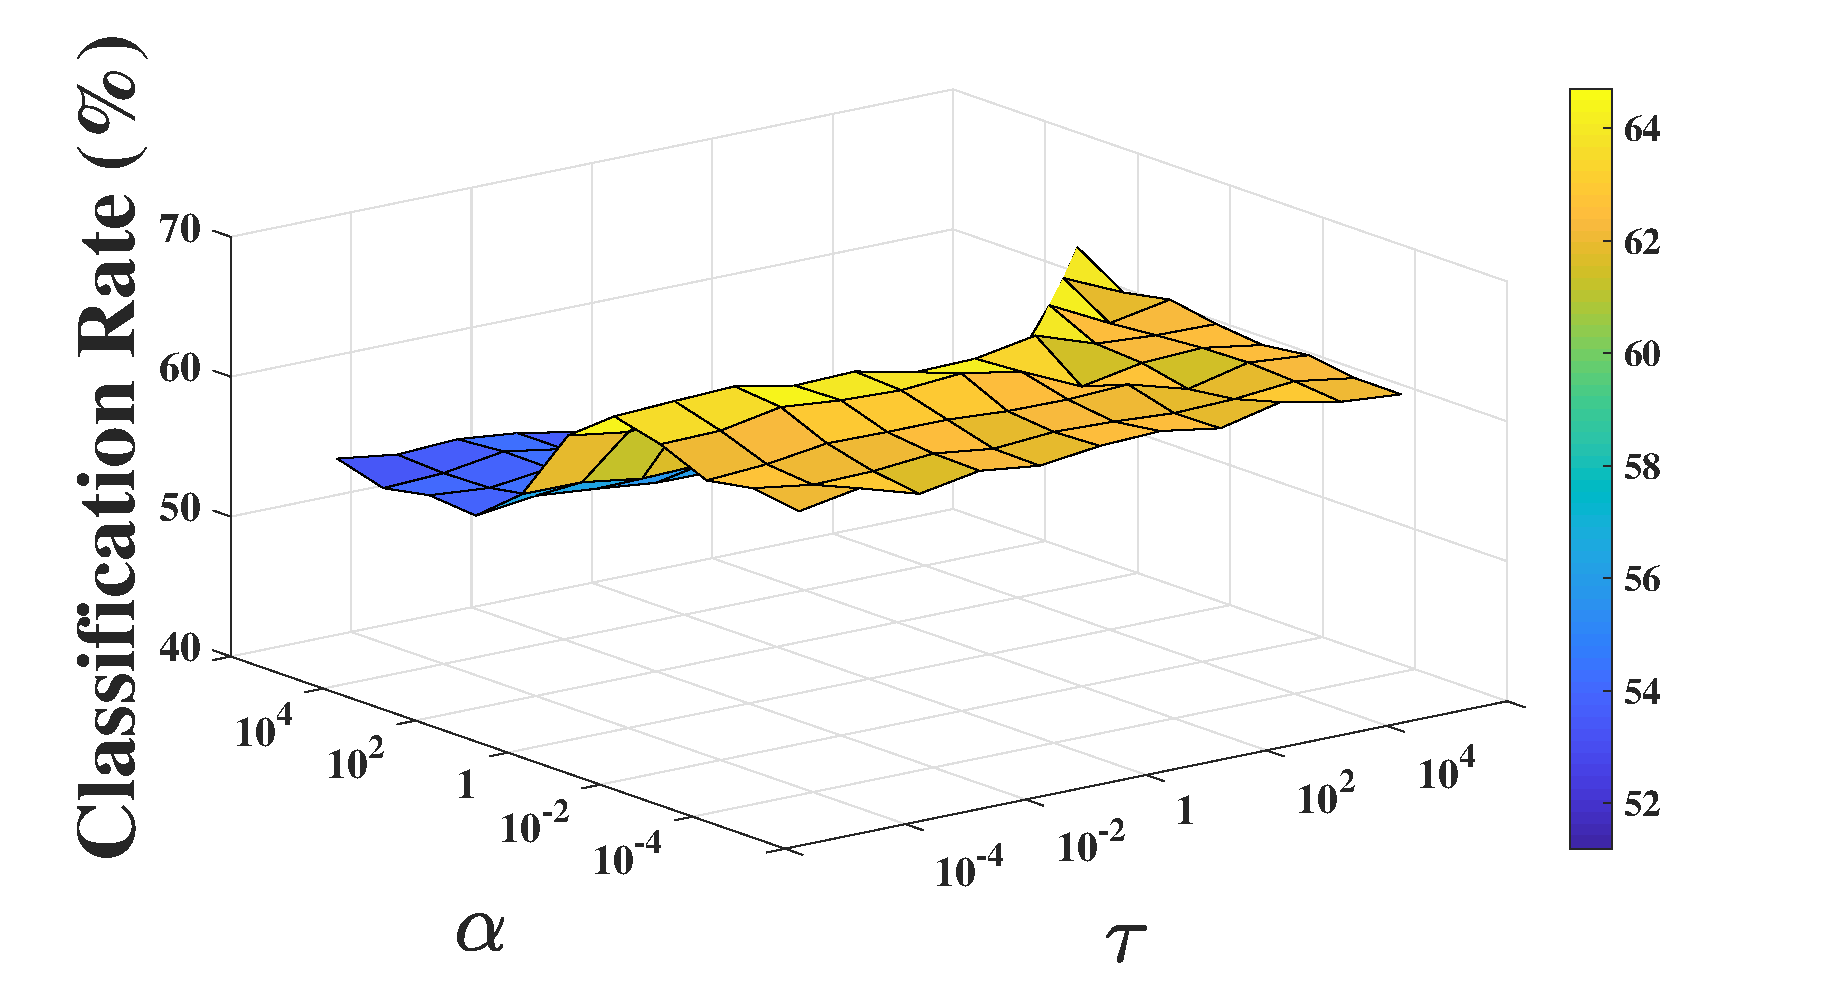
\includegraphics[keepaspectratio,width=0.45\textwidth,trim=0 0 0 0,clip]{figChap6/Fig_PFG_rate_alpha_tau.eps}} &
\subfigure[CMU PIE data set]{\label{fig:PIE_alpha_tau}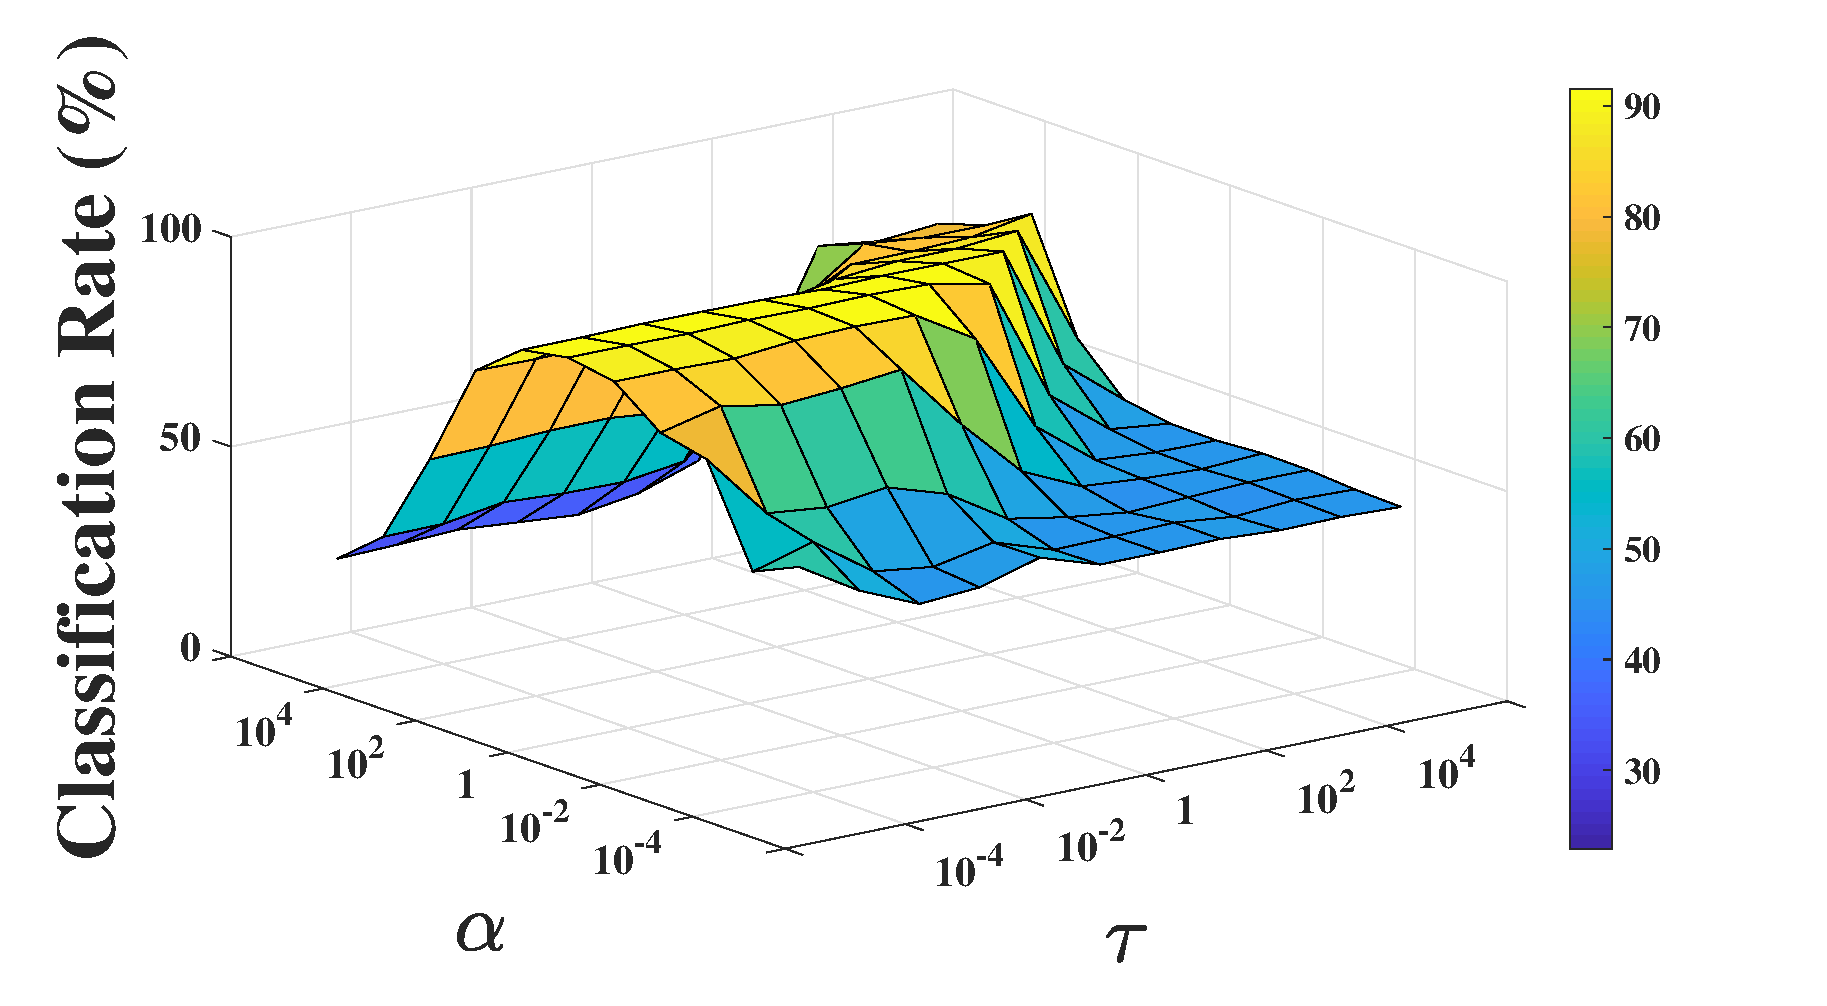
\includegraphics[keepaspectratio,width=0.45\textwidth,trim=0 0 0 0,clip]{figChap6/Fig_PIE_alpha_tau.eps}} 
  \end{tabular}
\caption{Mean classification rate ($\%$) of the proposed TRLSR method as a function of the parameters $\alpha$ and $\tau$ on different data sets.}
\label{fig: TRLSR_alpha_tau}
\end{figure}
%
%
%------------------------------%
\begin{figure}
\centering
    \subfigure[AR data set]{\label{fig: Coil_conv}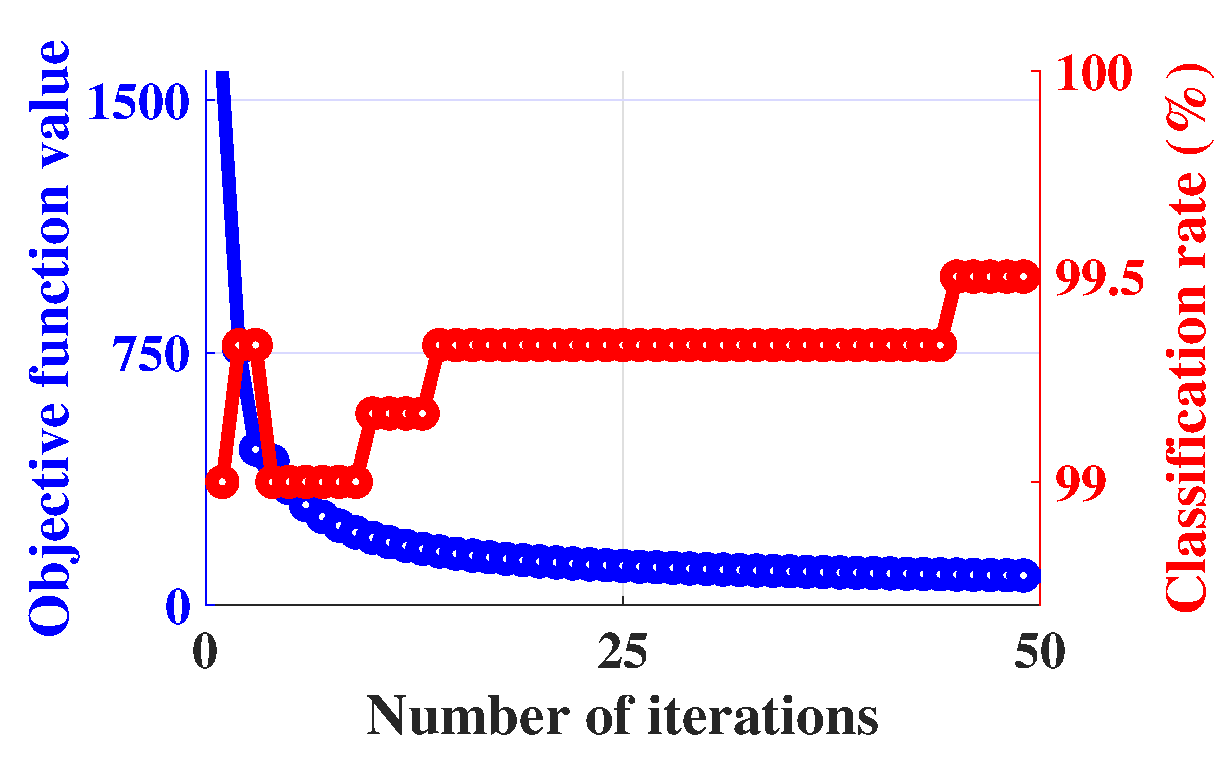
\includegraphics[width=.45\textwidth]{figChap6/PRL_AR_conv.eps}} 
    \subfigure[Ex Yale B data set]{\label{fig: Yale_conv}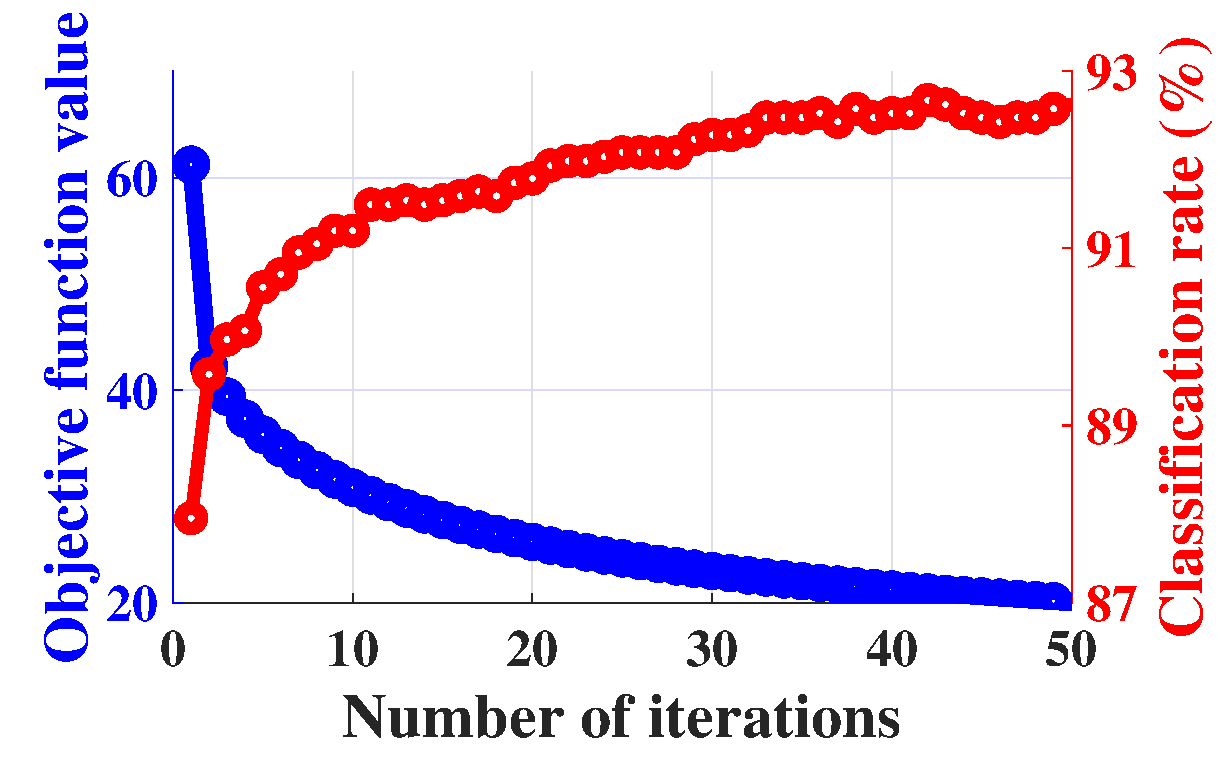
\includegraphics[width=.45\textwidth]{figChap6/PRL_yale_conv.eps}}  
\caption{Evolution of the objective function value and classification rate with the number of iterations for the proposed TRLSR method.}
\label{Fig: TRLSR_Data_conv}
\end{figure}
%%=======================================================%%
%
\subsection{Computational Complexity}
\label{sec:complexity}
%
In this section, we analyse the computational complexity of Algorithm~\ref{Algo: TRLSR}. In TRLSR, the computationally dominant operation is matrix inversion. To update projection matrix $\bm{Q}$, the computation of $\bm{X}\left( \bm{U} + \overline{\bm{M}} \right)^{T}$ has complexity $\mathcal{O} \left( nmc + nc\right)$ and computing the inverse of $\left( \bm{X} \bm{X}^{T} + \gamma \bm{Z} \right)$ has complexity $\mathcal{O}\left( m^{2}n + m \right)$. Thus, the overall complexity of updating $\bm{Q}$ is $\mathcal{O} \left( nm^{2} + m + nmc + nc\right)$. We ignore the complexity associated with the computation of $\bm{M}_{k}$ and $\overline{\bm{M}}$ as it only involves computing the mean vectors $\bm{m}_k$. For updating $\bm{U}$, the complexity is $\mathcal{O}\left(c^{3} + nmc + c^{2}n + c^{2}\right)$. Further, to update $\bm{V}$ the cost of matrix multiplication is $\mathcal{O}\left(c^{3} + 2c^{2}n + c\right)$ and updating $\bm{T}$ has complexity $\mathcal{O}(nc)$. In real world computer vision applications, typically $n \gg m$ and $m\gg c$, and hence, the overall computational complexity is $\mathcal{O} \left( nm^{2} \right)$. 

In DLSR, there are two key steps, namely matrix inversion with complexity $\mathcal{O}(2nm^{2} + m)$ and matrix multiplication with complexity $\mathcal{O}\left(2nmc \right)$~\cite{DLSR}, resulting in an overall complexity of $\mathcal{O}\left(nm^{2} + m + nmc \right)$. Similarly, in ReLSR, matrix inversion and multiplication are the key computational steps with overall complexity being $\mathcal{O} \left( nm^{2} + m + nmc + nc\right)$~\cite{ReLSR}. This computational complexity analysis shows that TRLSR has similar computational complexity as the state-of-the-art methods while achieving improved classification performance.
%
%===================================================%
\subsection{Convergence Study}
\label{subsec: TRLSR_conv_study}
Next, we study the convergence of Algorithm~\ref{Algo: TRLSR}.
%=================================================%
\begin{prop}
\label{prop: Prop_conv}
The optimization problem~\eqref{eq: TRLSR_Simple_formulation} is convex, where each sub-problem is convex with respect to the variables $\bm{Q}$, $\bm{U}$, $\bm{V}$, and $\bm{T}$.
\end{prop}
%
\begin{proof}
\label{proof: Convex_conv}
%
For the optimization problem~\eqref{eq: TRLSR_Simple_formulation}, the sub-problem with respect to $\bm{Q}$ is a sparse constrained optimization problem which is convex as the sparse $\ell_{2,1}$-norm is convex~\cite{DLSR}. For $\bm{U}$ and $\bm{V}$, the sub-problems are convex as their gradients exist and their Hessian matrices are positive semi-definite. The sub-problem with respect to $\bm{T}$ is a convex constrained quadratic programming problem \cite{ReLSR}. Therefore, the sub-problems with respect to $\bm{Q}$, $\bm{U}$, $\bm{V}$, and $\bm{T}$ are convex.
%
\end{proof}
%
The convergence results are shown in Fig.~\ref{Fig: TRLSR_Data_conv} where the objective function value and classification rate are shown as a function of the number of iterations on two data sets. It is seen that the objective function value decreases rapidly initially before asymptotically reaching its final value. The classification rate for the proposed method increases over the initial few iterations before saturating. For instance, the proposed method takes only $20$ and $25$ iterations to achieve a classification rate close to the final value on the AR and Ex Yale B data sets, respectively. These experiments show that the proposed TRLSR method converges rapidly and reaches a local optimum point.
%
%----- Tsne Visualization -------------%
\begin{figure}
\centering
 \begin{tabular}{@{}ccc@{}}
 \subfigure[\scriptsize{Original samples: Ex Yale B data set}]{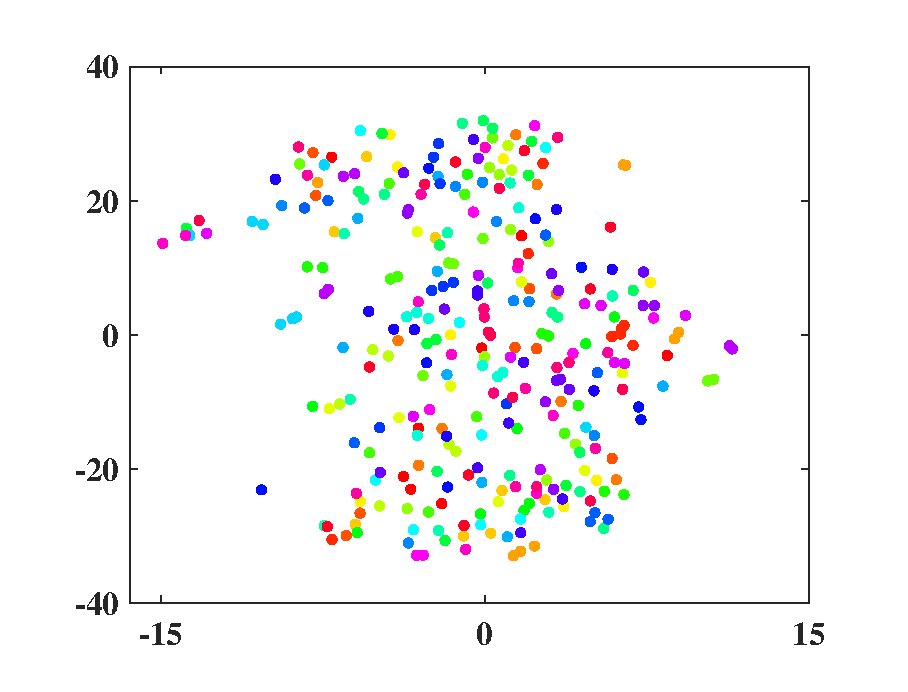
\includegraphics[width=.34\textwidth]{figChap6/PRL_yale_orig_tsne_10.eps}} &
 \subfigure[\scriptsize{Original samples: CMU PIE data set}]{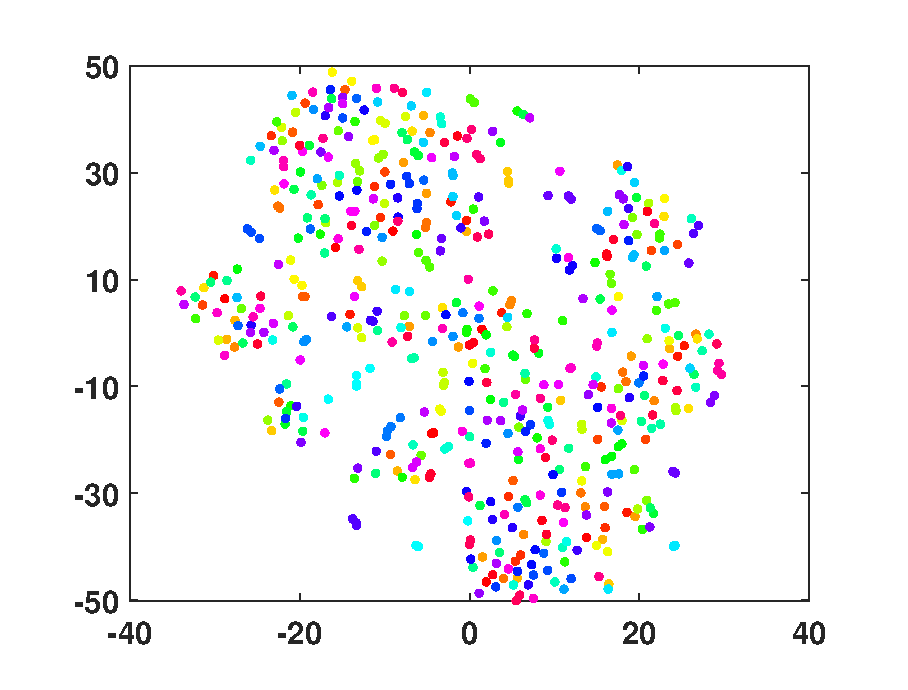
\includegraphics[width=.34\textwidth]{figChap6/PRL_PIE_orig_15.eps}}&
  \subfigure[\scriptsize{Original samples: PubFig83 data set}]{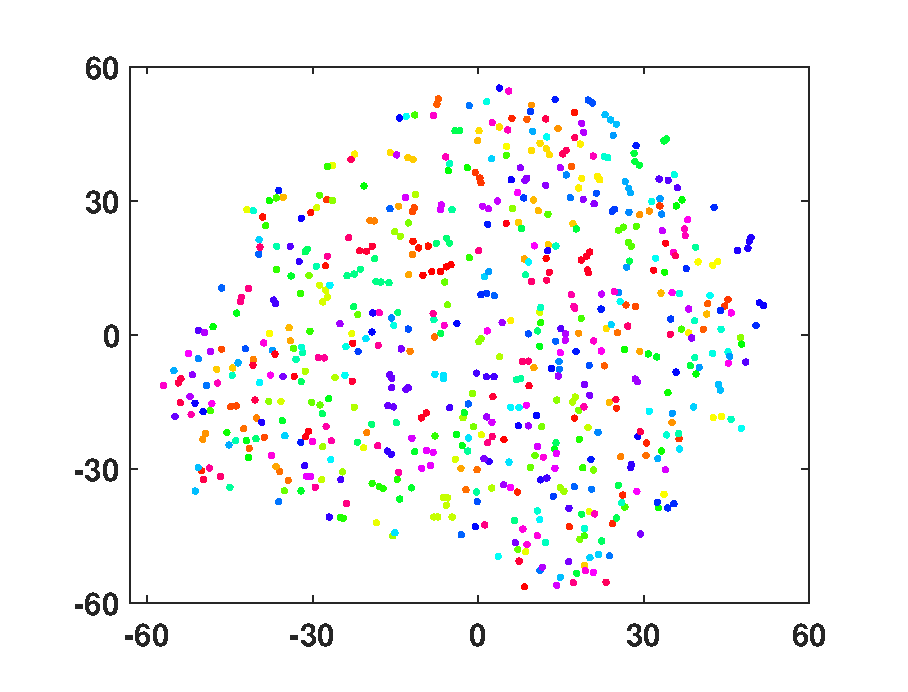
\includegraphics[width=.34\textwidth]{figChap6/PRL_PFG_orig_10_me_se_8.eps}}\\
  \subfigure[\scriptsize{Transformed features: Ex Yale B data set}]{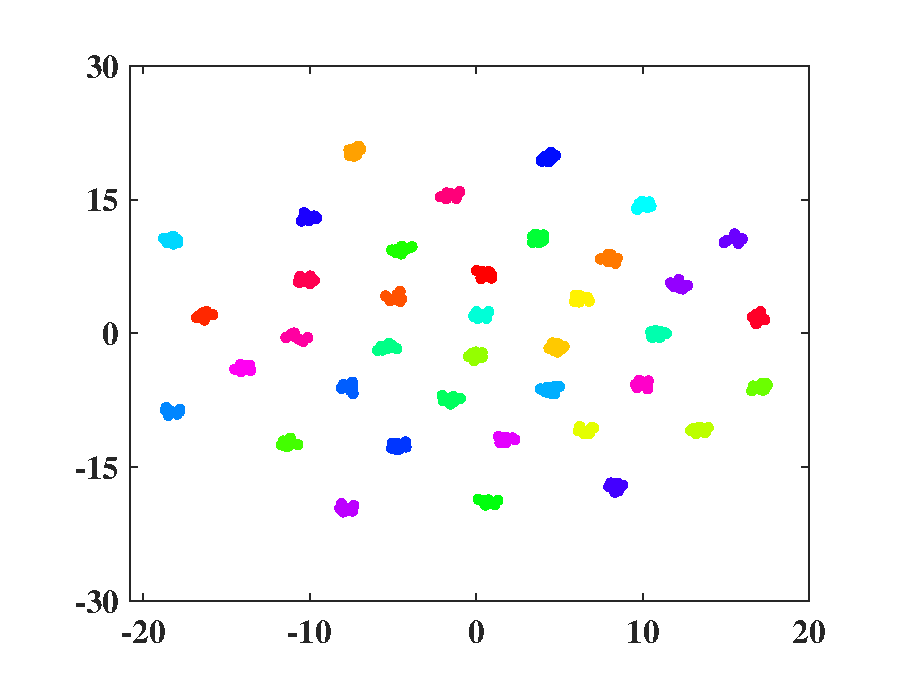
\includegraphics[width=.34\textwidth]{figChap6/PRL_YaleB_trans_10.eps}} &
  \subfigure[\scriptsize{Transformed features: CMU PIE data set}]{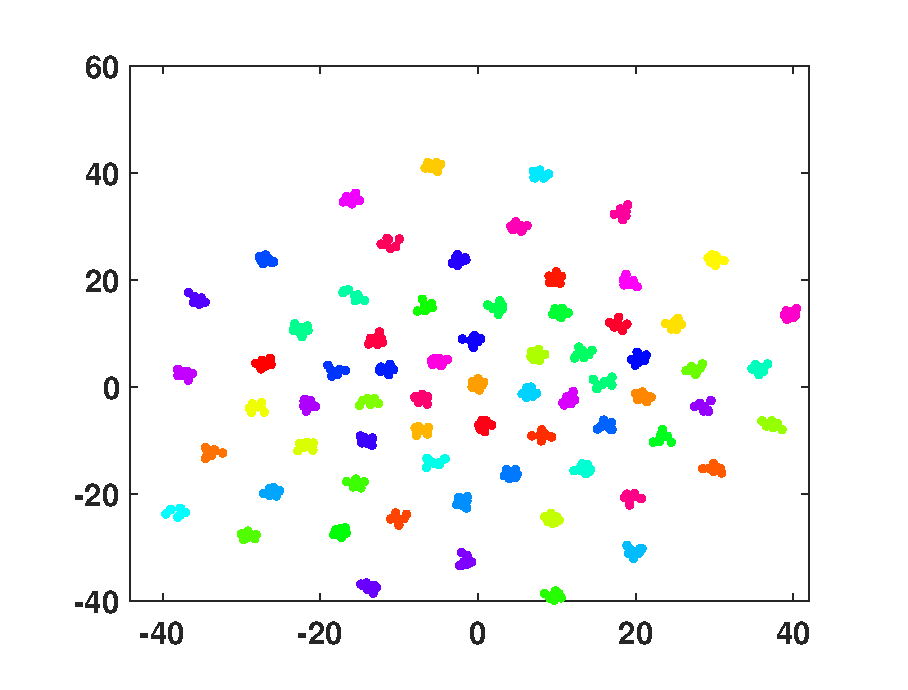
\includegraphics[width=.34\textwidth]{figChap6/PRL_PIE_trans_15.eps}}&
  \subfigure[\scriptsize{Transformed features: PubFig83 data set}]{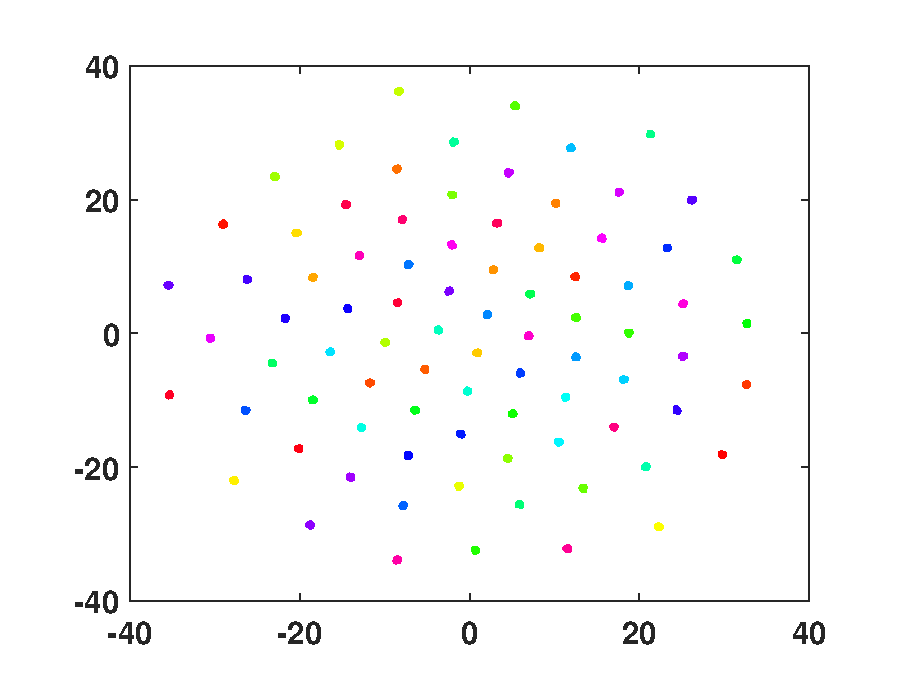
\includegraphics[width=.34\textwidth]{figChap6/PRL_Pfg_trans_10_me_se_8.eps}}
  \end{tabular}
\caption{t-SNE visualization of the original samples and transformed features obtained using TRLSR method for Ex Yale B ($t_r = 10$, validation = 8 samples/person), CMU PIE ($t_r=15$, validation = 10 samples/person), and PubFig83 ($t_r=15$, validation = 8 samples/person) data sets.}
\label{Fig: TRLSR_TSNE}
\end{figure}
%
\subsection{Remarks}
%
\begin{itemize}
%
\item The proposed TRLSR algorithm achieves the best performance in terms of classification rate compared to the state-of-the-art algorithms.
%
\item TRLSR outperforms DLSR and ReLSR methods on all the data sets. This is achieved by exploiting the intra-class correlation among the data samples and taking into account the local structure of the data.
%
\item TRLSR employs a relaxed target matrix along with a twin matrix for enlarged inter-class margin resulting in flexible and discriminative projection learning. The main difference between the proposed TRLSR method and ReLSR~\cite{ReLSR} and GReLSR~\cite{GReLSR} is that TRLSR shares the responsibility of relaxing the target matrix and preserving the data correlation using the twin matrix.
%
\item TRLSR incorporates a robust $\ell_{2,1}$-norm based regularization term for row sparsity. This curbs the influence of redundant features and noise, thereby avoiding overfitting. Thus, unlike~\cite{DLSR, ReLSR, GReLSR}, the proposed formulation can select more discriminative features.
%
\item To further demonstrate the efficacy of TRLSR, we visualize the distribution of the transformed features using the t-SNE algorithm~\cite{TSNE}. From Fig.~\ref{Fig: TRLSR_TSNE}, it is seen that TRLSR efficiently classifies the data samples into their respective subspaces by capturing discriminative and compact features from the original data samples. It also shows that the features captured using TRLSR increase both the intra-class similarity and the inter-class margins.
%
\end{itemize}
%
\section{Chapter Summary}
\label{sec: TRLSR_conclusion}
%
In this chapter, we presented two frameworks for regression based feature extraction. First, we proposed a low-rank double relaxed regression (LR-DRR) based discriminative projection learning model for image classification tasks. LR-DRR provides double relaxation to the regression framework by learning a relaxed target matrix with greater degrees of freedom.  Further, LR-DRR includes a term with low-rank constraint on the label error matrix so as to learn the underlying structure of the data. Next, we presented a new twin relaxed least squares regression (TRLSR) model for multi-class image classification. The proposed approach jointly learns a relaxed target matrix and a twin matrix, with structural mapping between the two, for enlarged inter-class margins and improved classification. Unlike most existing methods, TRLSR incorporates a twin matrix with intra-class similarity constraint to exploit the underlying data correlation. Hence, the proposed method is more effective in preserving the intrinsic neighbor relationships within each class. Additionally, TRLSR incorporates an $\ell_{2,1}$-norm based regularization for the projection matrix, which allows selection of the most discriminative projections from the high-dimensional data. Extensive performance analysis of LR-DRR and TRLSR methods on several public data sets demonstrate the effectiveness and wide applicability of the proposed algorithms.
%